\documentclass[letterpaper,12pt,titlepage]{article}

\title{MQP Report}


\usepackage[table]{xcolor}
\usepackage[top=1in, bottom=1in, left=1in, right=1in]{geometry}
\usepackage{minted}
\usepackage{mdwlist}
\usepackage{tikz}
\usepackage{pdfpages}
\usepackage{ragged2e}
\usepackage{mathtools}
\usepackage[titletoc,title]{appendix}
\usepackage{subfiles}
\usepackage{mathcomp}
\usepackage{graphicx}
\usepackage{cite}
\usepackage{titlesec}
\usepackage[nomessages]{fp}
\usepackage{pdfpages}
% \usepackage[sorting=nyt,firstinits=true]{biblatex}
\graphicspath{{./Pictures/}}

% add subsubsubsection as a command
\newcommand{\subsubsubsection}[1]{\paragraph{#1}\mbox{}\\}
\setcounter{secnumdepth}{4}
\setcounter{tocdepth}{5}

\usepackage[]{hyperref}
\hypersetup{
    pdftitle={},
    pdfauthor={},
    pdfsubject={},
    pdfkeywords={},
    bookmarksnumbered=true,     
    bookmarksopen=true,         
    bookmarksopenlevel=1,       
    colorlinks=false,            
    pdfstartview=Fit,           
}

\renewenvironment{description}%
{
\begin{basedescript}{
\desclabelstyle{\nextlinelabel}
\renewcommand{\makelabel}[1]{%
\parbox[b]{\textwidth}{\bfseries##1}%
}%
\desclabelwidth{2em}}}
{
\end{basedescript}
}

\setlength{\parindent}{4em}
\setlength{\parskip}{1em}
\setlength{\tabcolsep}{10pt}
\renewcommand{\arraystretch}{1.2}

%Build the custom title page.
\begin{document}
\begin{titlepage}
\pagenumbering{Alph}
\begin{center}
\begin{minipage}{\textwidth}
\centering

\includegraphics[scale=0.1]{WPI_Inst_Prim_FulClr.png}

\LARGE
\textsc{Worcester Polytechnic Institute}
\vspace*{0.5cm}
\noindent\rule{\textwidth}{1pt}
\Huge
\textbf{MIRA} \\
\LARGE
\textsc{Modular Interchangeable Robotic Arm}
\vspace*{0.5cm}
\noindent\rule{\textwidth}{1pt}
\end{minipage}

\vspace{2cm}
\vfill    

\Large
\textbf{Submitted on} \\
\large
April 25, 2018\\
\vspace{0.8cm}
\Large
\textbf{Submitted by} \\
\large
Chris O'Shea, RBE\\
\large
Alex Taglieri, RBE/CS \\
\large
Ben Titus, RBE/ECE \\
\vspace{0.8cm}
\Large
\textbf{Advised by} \\
\large
Susan Jarvis \\
\large
Craig Putnam \\
    
\vfill
\end{center}

\normalsize
\noindent \textit{This report represents the work of one or more WPI undergraduate students submitted to the faculty as evidence of completion of a degree requirement. WPI routinely publishes these reports on its web site without editorial or peer review}
\end{titlepage}

%%%% Document begins here %%%%
\newpage
	\pagenumbering{roman}
	\noindent \textbf{\Large Abstract} \\
%\vspace*{0.5cm)
\noindent Low-cost robotic arms are becoming much more popular in educational settings. The goal of this project is to create a proof of concept for a modular robotic arm. To accomplish this, we have modified an existing arm to use our own modular control system, created a removable joint that can be connected to the end of the arm, and created an end-user interface which allows visualization of the arm’s movement in real time. Creating this arm will make robotics education accessible to a larger number of people, without compromising the potential for each person to gain a high quality understanding of the way robotic arms behave. \\
\newpage
	\tableofcontents
	\newpage
	\listoffigures
	\newpage
	\listoftables
\newpage

\pagenumbering{arabic}
\noindent \newline 
\textbf{Abstract}
Low-cost robotic arms are becoming much more popular in educational settings. The goal of this project is to create a proof of concept for a modular robotic arm. To accomplish this, we have modified an existing arm to use our own modular control system, created a removable joint that can be connected to the end of the arm, and created an end-user interface which allows visualization of the arm’s movement in real time. Creating this arm will make robotics education accessible to a larger number of people, without compromising the potential for each person to gain a high quality understanding of the way robotic arms behave. \\
\newpage

\section{Introduction} 
% Section outline:
% Overall summary of project - ~1 sentence per major goal
% ~1 Paragraph for each major goal
% Paragraph at end describing what is in this document

%Designed by Kevin Harrington in Bowler Studio
\subsection{Problem Statement}
\noindent Currently, it is difficult for users to fully understand the motion of robotic arms and the kinematics that control them. This understanding is a crucial step in working with robotic arms safely and efficiently, but is often lacking due to the inability of diagrams and descriptions to fully convey what makes one arm operate differently than another. With the use of robotic arms becoming more common and the many different kinds of arms available, it is important to have a prototyping platform that can emulate many different kinds of arms so that the user can gain a better grasp of what components make up a robotic arm why one arm is better suited for a particular use case than another.

\subsection{Goal Statement}
The goal of this project is to create a proof of concept of an arm that can be reconfigured by end users such that they can create many different types of functionality from one set of principal components. To accomplish this, we need to break the arm down into small modularized joints that can be rearranged to show how the combination of different kinds of joints can lead to a specific end result. We also need to create an adaptable electrical system that is able to modularly control each different joint by having the capability to handle multiple types of sensors and actuators. By doing so, we hope to take the first step into creating a standardized kit of parts and the software accompanying it to prototype almost any type of arm that is currently used. 

\subsection{Objectives}
\noindent In order to measure our progress, we need to define a set of objectives that we need to accomplish in order to meet our goals outlined above. To create a proof of concept of a modular robotic arm prototyping platform, we set the following objectives: 
%\newline \noindent \textbf{Objectives}
\begin{itemize}
\item Define commonly used robotic arms and their uses.
\item Understand the variety of different joints and what sensors and actuators are used to control them.
\item Understand how the combinations of different joints affects the kinematics of the arm.
\item Classify several different standardized joints and what sensors/actuators make them work.
\item Create a control bus made up of connected joints with a node at each joint capable of controlling any single joint.
\item Create a joint that can be added and removed from an existing arm in order to modify the arm's functionality.
\item Create an arm control board which functions as an interface between a computer and our arm's control bus allowing for users to interact with the arm through a software interface.
\item Create a software application which displays information about the arm in real time and allows users to easily set up their arm and send it commands.
\end{itemize} 

\subsection{Constraints}
\noindent In order to complete this project in the alloted time, we had to place limits on our goals for the project. One such constraint was taking into account the time it would take to prototype, design and assemble a fully modular arm from scratch. To handle this, we decided that we could show off a smaller-scale example of modularity by modifying an existing arm by adding a joint that can be easily removed. By fully creating our own link that can be attached to the arm to increase utility, we proved that the idea of a modular joint is feasible and therefore those joints can be combined to create a modular arm. We also had to impose another constraint to ensure proper functionality of the arm which is that the arm can have at maximum six joints controlled at once. This constraint was decided based upon examples of other robotic arms as well as a way to make sure that the arm is structurally sound and within weight tolerances.

\subsection{Summary}
\noindent Once we outlined our goals and constraints for the project, we had a clear idea of where to start researching. Knowing what we have to accomplish as well as knowing the obstacles standing in our way, we were able to approach the project piece by piece, working towards our goals as well as keeping a solid perspective about the entire scope of the project. When we ran into design decisions that were not foreseeable before we got working, we referred back to our original goals and based our decisions off of these initial measures of project progress. Moving forward after defining the problem fully and how we wanted to accomplish it, we proceeded to conduct research on current robotic arm technology that we used as a reference for our arm.  

%The goal of this project was to create an adaptable control system whose purpose is to drive a variety of robotic arms. To prove the usefulness of our system, we retrofitted an existing robot arm from the RBE 3001 course with our control system. In addition to this, we modified the existing arm to include an interchangeable joint on the end of our arm, controlled by our system. To interface with our system, we created a GUI for easy configuration and basic control of the arm. The base communicates with a computer running control code through the software application. \\
%\newline
%
%\begin{figure}[H]
%\centering
%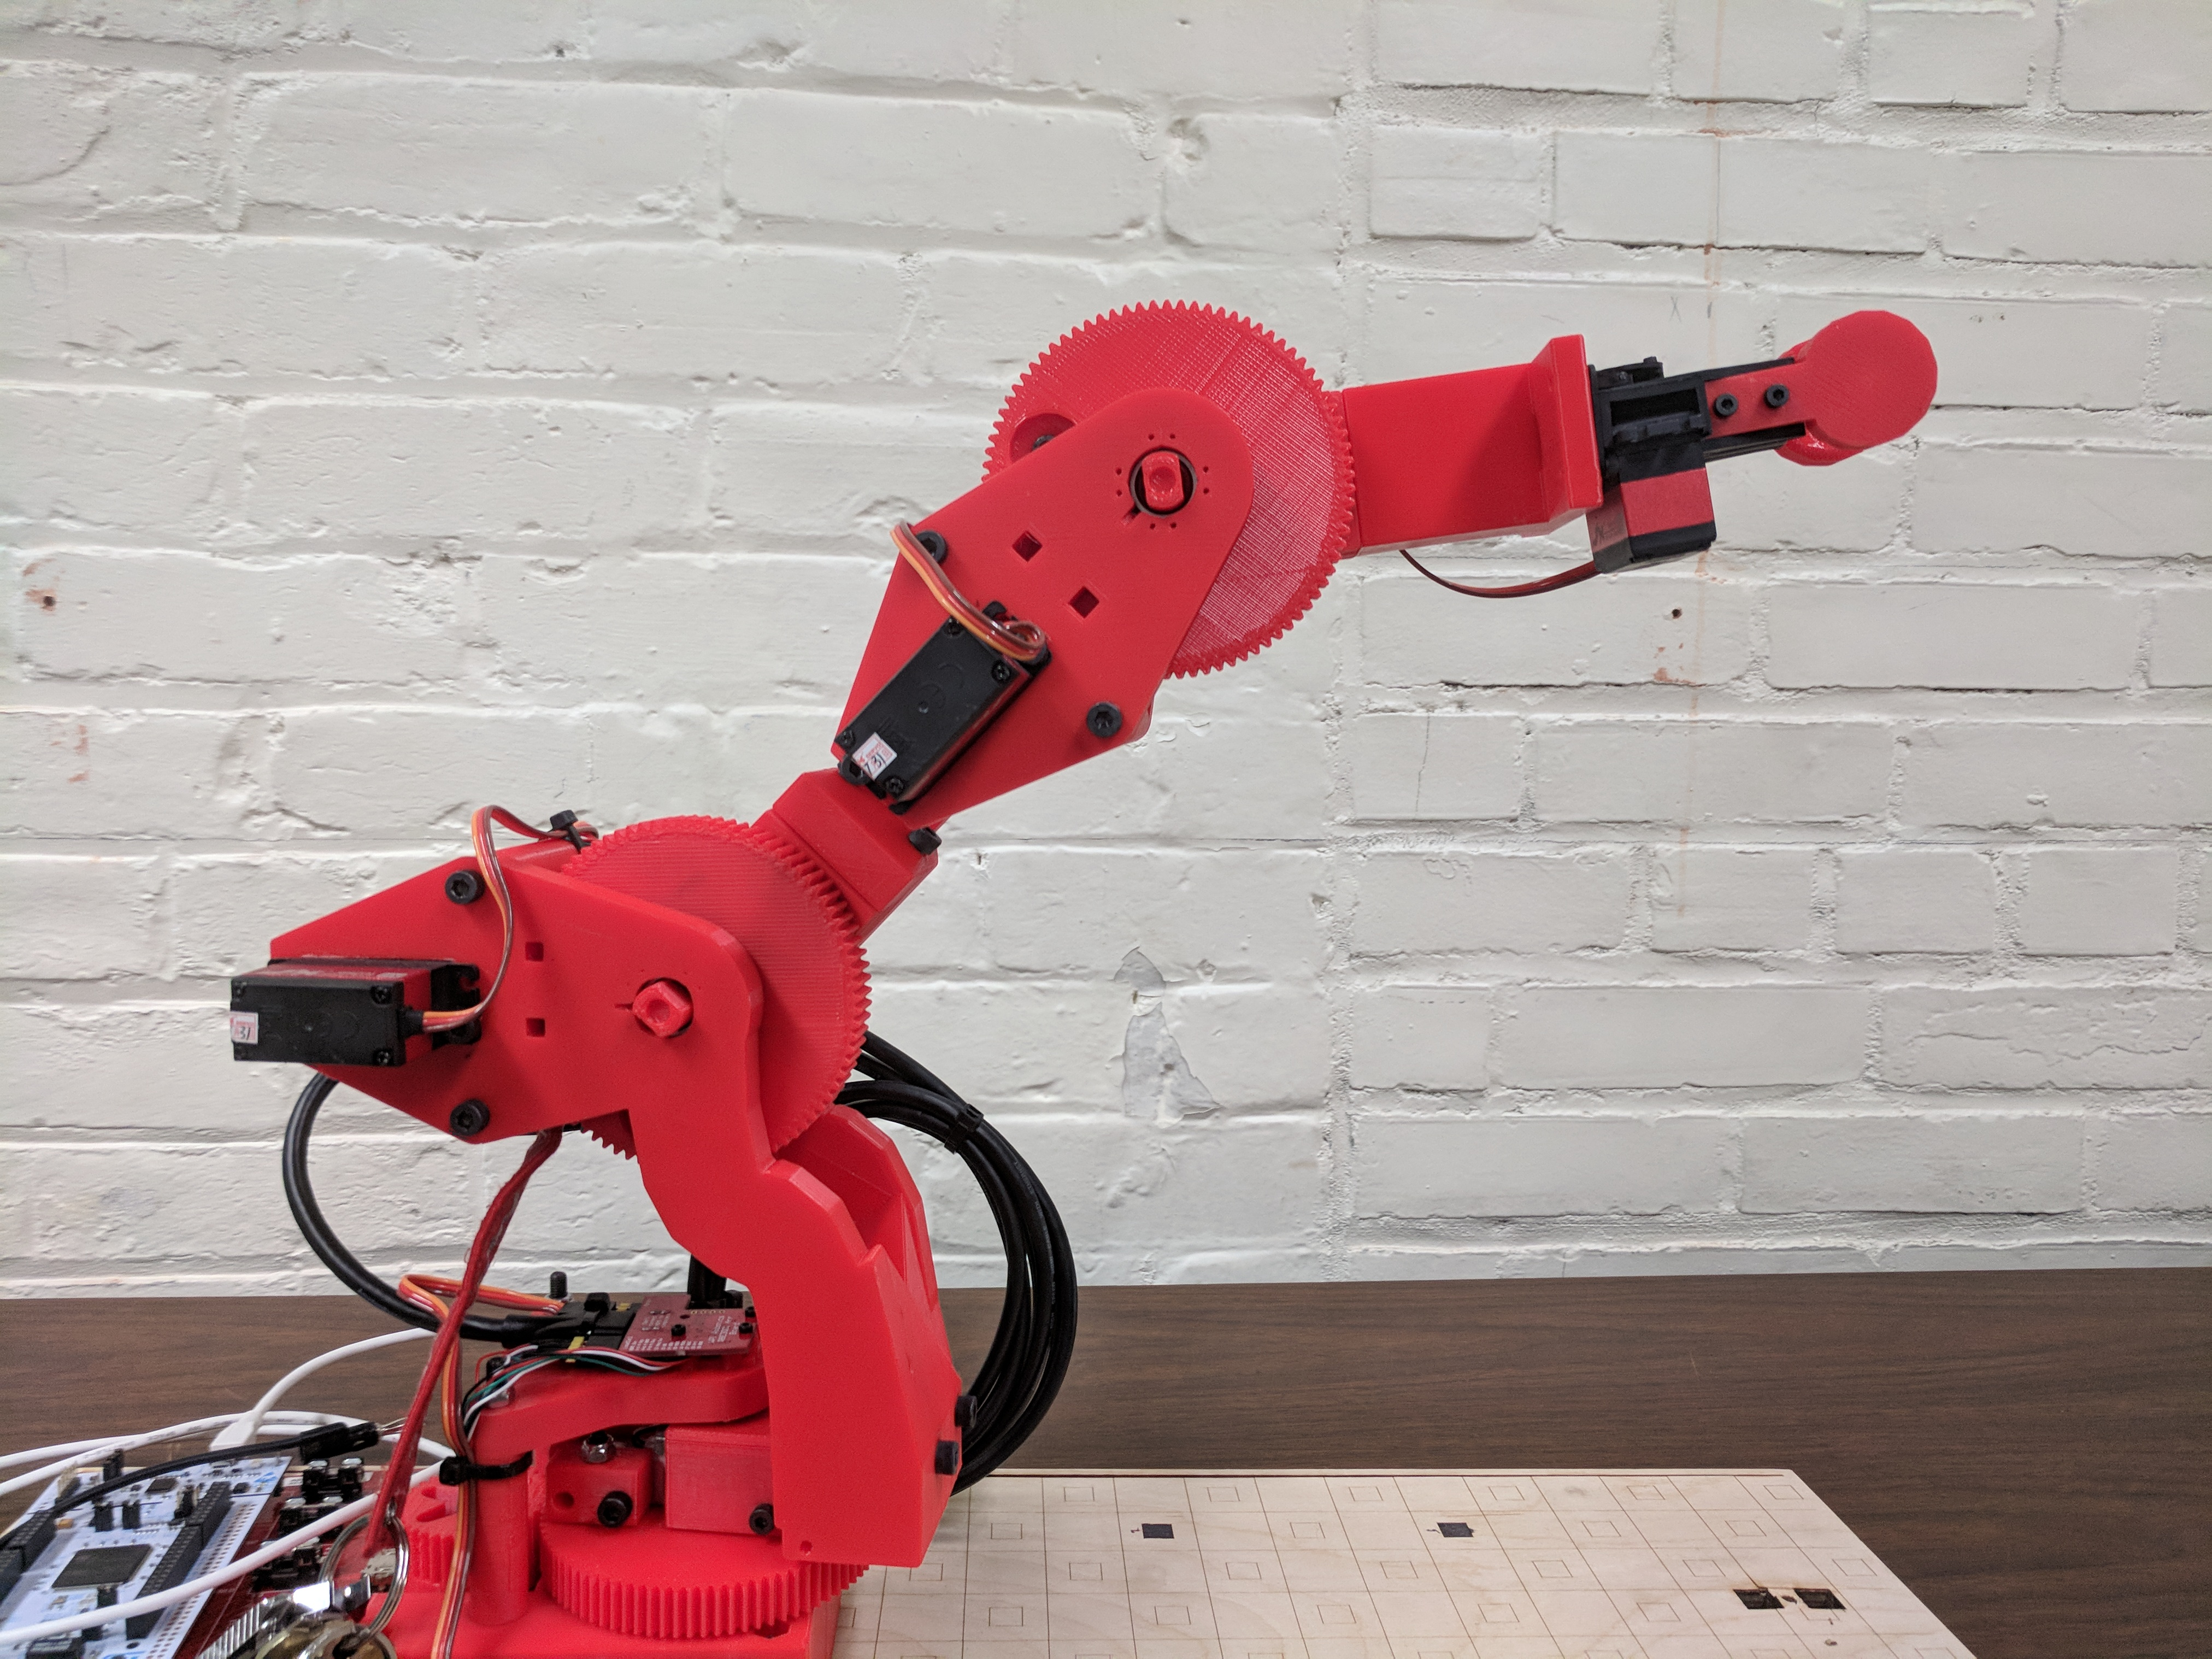
\includegraphics[width=\textwidth]{Initial_3001_Arm}
%\caption{Unmodified RBE 3001 Arm}
%\label{fig:3001_Arm}
%\end{figure}
%
%
%
%\noindent The existing RBE 3001 arm already has its own central control system. We removed this and replaced it with our own distributed one. To accomplish this, we designed a joint control board that communicates with a base controller.  We also designed and implemented a new joint on the arm. This new joint is interchangeable to prove that our software and control system will work with more than one configuration. The joint implements our control board. \\
%\newline
%We created a software application to interface with a constructed arm. The user inputs how they have configured their arm into this application and are then able to do some simple control. Another feature of this application is the ability to record a series of poses for the arm to perform. In addition to this software, we also created some programming libraries to allow users to control the arm with their own programs. \\
%\newline
%In this document, we will outline some existing robot arms and highlight the differences between these arms and our arm kit. We then discuss what work there is to be done on this project. After discussing the work to be done, we state how this work will satisfy the capstone design requirements for each of the three disciplines represented by our group members. Then, we state the constraints we expect going forward with this project. Next, the acceptance criteria for any deliverables at the end of this project will be outlined. Finally, we will state an estimated time line for this project. Additionally, due to changes in project organization we have significantly changed the scope and goals of the project. See Appendix \ref{app:Early-Project-Iteration} for more information about this earlier iteration of our project.
\section{Background}
% Section outline
% Overall summary of section - ~1 sentence per major topic
% ~1 Paragraph for each major topic
\subsection{Introduction}
In this section we will begin with an overview of some existing robotic arms that are currently in industry use in order to gain a high level understanding of what different kinds of arms are out there. Researching the various use cases of existing robotic arms can help us define use cases for our arm. Next, we discuss modular arm technology that is in development in order to have a measure of our progress versus their projects. After examining these arms, we highlight how our project is different from the previously discussed examples and why this is important. Finally, we discuss some of the technology that had to be researched in order to inform our decision on how to design our arm and choose components.

\subsection{Examples of Robot Arms}
There are a few different types of robot arms available on the market today.  Industrial robotic arms, the most common type of arm currently in use are defined as robotic systems used for manufacturing by means of an end effector. Since our arm is relatively small and handles lighter payloads compared to most industrial arms, we will begin with an overview of existing "desktop" industrial arms. Arms that fit this description have a reach of less than one meter. Industrial robot arms typically cost between \$50,000 to \$80,000 new and \$25,000 to \$40,000 used \cite{RobotWorx}. Some manufacturers of these industrial arms include ABB Robotics, Universal Robots, and KUKA Robotics. It's important to note that none of these arms are modular - in fact, they can't be changed at all!

\subsubsection{ABB Robotics}
ABB Robotics makes many small industrial arms. The ABB IRB 120 boasts a 580mm reach, 3kg payload, and 25kg weight. It has 6 degrees of freedom and can be mounted at any angle. The ABB IRB 1200 comes in two varieties, one with a 703mm reach and 7kg payload, and one with a 901mm reach and 5kg payload. Both of these arms have 6 degrees of freedom. The weights are similar at 52kg and 54kg respectively \cite{RobotWorx}.

\begin{figure}[H]
\centering
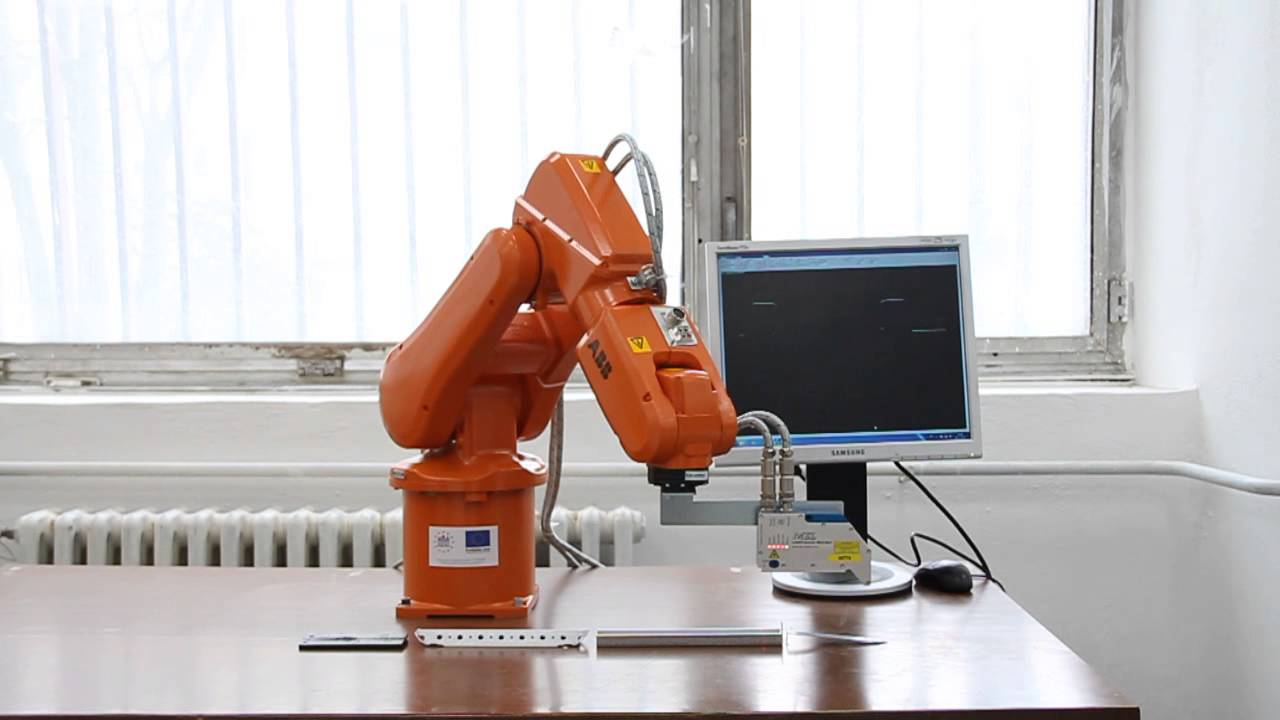
\includegraphics[width=\textwidth]{ABB-irb-120}
\caption{ABB IRB 120 arm \cite{IRB_120}}
\label{fig:abb-irb-120}
\end{figure}

\subsubsection{Universal Robots}
Universal Robots makes two robot arms in this size range. The UR3 is the smaller of the two with a reach of 500mm, payload of 3kg, and 11kg weight. A step up is the UR5 which has a 850mm reach, 5kg payload, and 18.1kg weight. Both of these arms have 6 degrees of freedom. Universal boasts that these arms are easy to implement and re-implement due to compact and lightweight construction, and simple programming interface \cite{RobotWorx}.

\subsubsection{KUKA AG}
KUKA makes two robot arms in this size range. The KR3 R540 has a reach of 541mm, payload of 3kg, and weight of 26kg. It can be mounted on the floor, wall, or ceiling for added utility. The KR 5 sixx R650 is larger with a reach of 650mm, payload of 5kg, and weight of 127kg. It can only be mounted on the floor or ceiling. Both of these arms have 6 degrees of freedom \cite{RobotWorx}.

\subsubsection{Small Industrial Robotic Arm Comparison}
Table \ref{tab:ArmComparison} shows a comparison of all the robotic arms discussed in this section.
\begin{table} [H]
	\centering
	\caption{Comparison of $<$1000mm reach industrial robot arms}
	\label{tab:ArmComparison}
	\begin{tabular}{| l | c | c | c | c |}
		\hline
		\textbf{Name} & \textbf{Reach (mm)} & \textbf{Payload (kg)} & \textbf{Weight (kg)} & \textbf{Axes} \\
		\hline
		IRB120 & 580 & 3 & 25 & 6 \\
		IRB1200-7/0.7 & 703 & 7 & 52 & 6 \\
		IRB1200-5/0.9 & 901 & 5 & 54 & 6 \\
		UR3 & 500 & 3 & 11 & 6 \\
		UR5 & 850 & 5 & 18.1 & 6 \\
		KR3 R540 & 541 & 3 & 26 & 6 \\
		K5 sixx R650 & 650 & 5 & 127 & 6 \\
		\hline
	\end{tabular}
\end{table}

\subsection{Modular Arms}
While there are many industrial arms in production, there are very few modular robotic arms. There is one commercially available robotic arm, the Robolink, made by igus. A few modular robot arms have been developed, including the reconfigurable modular manipulator (RMM), made by TRACLabs \cite{RMM}, and a single joint for the Modular Robotic Arm project MQP at WPI \cite{MRA}.

\subsubsection{igus Robolink} 
Robolink is a modular robotic arm kit produced by the plastics manufacturing company igus.  The kit contains parts to make an arm that is up to 6 Degrees of Freedom (DOF), with belt driven linkages powered by stepper motors that reside in the base of the robot.  Robolink offers 7 individual links, ranging from 1-2 DOF and differing based upon their kind of motion (pivoting, rotating, swiveling).  Each link is made of a lightweight and strong plastic or carbon fiber with cables inlaid in them, resulting in a low cost and weight arm.  The cables used to control these links are made of a high strength synthetic fiber with has a tensile strength of 4,000N.  Separating the actuation of each link from the joint allows the arms to be easily maneuverable with its lightweight and strong joints.  \\
\newline
Purchasers of the kit are able to combine the links in different ways, allowing for a flexible, modular solution to robotic arms. Igus also offers their Robolink software for programming articulated arms that facilitates the programming of individual arms through the use of a simple, intuitive control software. The total cost of a kit to make a 6 DOF arm is \$6000, and buying individual links will cost anywhere from \$370 to \$750 per link. While this price may be low cost compared to other arms such as the ABB robotic arm which can cost up to \$200,000 in total, it is still not low enough for either hobbyists or people interested in learning about robotic arms who are prevented from doing so by the high entry cost. In addition to this, the belt system actuating each link requires the user to thread belts attached to the actuators to each link in order to set up the robot. The long assembly time and intricacy also detracts from the idea of modularity because the time involved in switching configurations can inhibit users from really exploring the different workspaces and combinations this kit can create \cite{igus}.  

\subsubsection{Reconfigurable Modular Manipulator}
The reconfigurable modular manipulator developed by TRACLabs for NASA is a fully modular 7-DOF robot arm. Each joint and end effector have the same connector that provides power and control lines throughout the arm. Internal power and control circuitry take in these lines and convert them into movement. Joints can be swapped out by hand in a matter of seconds. Joints accept position or velocity data from the central communication lines and store physical characteristics about the joints in memory. This robot arm is not commercially available \cite{RMM}.

\subsubsection{Modular Robotic Arm}
This project aimed to close the market gap between inexpensive toy robot arms and expensive professional grade industrial arms. The group aimed to do this by designing a single joint that could be used to assemble a robot arm. Ultimately, a single DOF joint that was heavy, difficult to manufacture, and expensive to produce was designed and constructed. In their future recommendations section, the group stated that the goal of designing a modular robot arm was possible but their design was not the solution \cite{MRA}.

\subsection{Our Robotic Arm System}
Our modular robotic arm aims to offer a completely different use case compared to existing products. The system maintains a low cost while providing a versatile platform for anyone from novice engineers to rapid prototyping professionals. We accomplished this by avoiding expensive proprietary software and subtractive manufacturing; favoring off-the-shelf parts, 3D-printed structures, and freely available/open source software. Providing custom-built software for controlling the arm creates a plug-and-play environment suitable for most any skill level.

\subsection{Technology}
After examining all of these different robot arms accomplished their respective tasks, it was important to go a little more in-depth on how some very crucial components of any robotic arm are chosen and what that means for our project. Some of the most important ideas of an arm are: where does the central processing happen? How can we tell what both the position of and the force on each joint are? It is questions like these that led us to research these key functionalities so that we could make the right choice when we design our arm.  

% \subsection{Communications}
% We looked at several types of communications for the purposes of controlling our robotic arm. These include serial UART, SPI, I2C, and CAN. 
% \subsubsection{Controller Area Network}
% A controller area network (CAN) is a system for sending data reliably between distinct subsystems with reasonably low danger of transmission errors. CAN buses are widely used in the automotive industry to allow various computerized parts of the car to talk to one another.

% Research begins here?
\subsection{Control board}
The control board is meant to be implemented as an independent module that interfaces with a main controller module. Its tasks are to send and receive data from the main controller and control the position of a single motor. As such, the main factors that must be taken into account when designing the control board are methods of measuring joint position and motor torque, as well as communicate with an off-board controller. Motor torque is proportional to motor current. Therefore, the motor torque will be calculated from the measured current through the motor.
\subsubsection{Joint Position Detection}
Angular position sensing must be used to determine the joint angle of the motor. There are several commonly used methods of determining angular position, including potentiometers, optical encoders, and Hall effect sensors \cite{Pot_vs_Sensor,Choose_Sensor_Technology,Choose_Position_Sensor}. A comparison of the different angular sensors can be seen in Table \ref{tbl:Angular_pos_sensors}. \\
\newline
Potentiometers are very commonly used to measure angular position due to their simple implementation and low cost. In addition to being low cost, potentiometers provide high linearity and accuracy \cite{Choose_Position_Sensor}. Although generally robust, these sensors do not lend themselves well to many, rapid adjustments or mechanical vibrations. Both of these significantly reduce the lifespan of the sensor \cite{Pot_vs_Sensor,Choose_Position_Sensor}. The situations potentiometers excel in are those that require an easily adjustable voltage at low to medium adjustment frequencies, such as settings knobs on control panels or analog reference voltages as trim potentiometers \cite{Pot_vs_Sensor}. \\
\newline
Hall Effect sensors are less commonly used, and consist of a bipolar magnet rotating above a Hall effect sensor with the axis of rotation perpendicular to the plane of the sensor. Since there is no contact between the rotation and the sensor, these types of sensors have very long lifespans \cite{Pot_vs_Sensor}. Unfortunately, these sensors do not provide high resolution since they are susceptible to electromagnetic interference and temperature, and also have some hysteresis \cite{Choose_Position_Sensor}. \\
\newline
Optical encoders are another method of measuring angular position. These sensors consist of a beam of light that shines on a slotted disk so that as the disk rotates, the slots break the light beam. These sensors can have very high resolutions and are resistant to shock and vibrations \cite{Choose_Sensor_Technology}. Like magnetic sensors, these sensors have very long lifespans since there is no mechanical connection on the sensor \cite{Pot_vs_Sensor}. Unfortunately, these sensors are susceptible to foreign particles blocking the light beam from sensing the slots and causing incorrect readings. The most common kind of optical encoder, the Quadrature encoder, does not sense absolute position; it can only read relative position, meaning that a quadrature encoder would need to be combined with some other sensor in order for the robot to be able to sense its joint angles correctly. Other encoders called Absolute Optical Encoders do not have trouble reading absolute position, but they are prohibitively expensive. \cite{Choose_Position_Sensor}. \\
\newline
It's worth noting that limit switches can be used to provide information about the location of a joint. Limit switches give a different voltage depending on whether they are pressed or not. When a limit switch is placed at the edge of a particular mechanism's travel range, it becomes possible to determine when the mechanism has reached one of its limits of travel. \\
\newline
Limit switches can be used in conjunction with quadrature encoders (which only provide relative, rather than absolute, position) to create a system which is capable of determining its absolute position. The system would need to go through a homing process at startup whereby the mechanism travels until the limit switch is pressed, at which point the encoders treat their current position as "home".

\begin{table}[H]
	\begin{center}
		\caption{Comparison of different angular position sensors}
		\label{tbl:Angular_pos_sensors}
		\begin{tabular}{ | p{2.4cm} | r | p{1.6cm} | l | l | p{2.5cm} |}
			\hline
			Sensor & Cost & Linearity & Accuracy & Lifespan & Notes
			\\ \hline
			Potentiometer & \$ & Depends on ADC & Moderate & Short & Repeated motion at the same angle can lead to failure
			\\ \hline
			Encoder & \$\$\$ & Very High & Very High & Long & Inexpensive encoders can't sense absolute position
			\\ \hline
			Hall Effect Sensor & \$\$ & High & High & Very Long & Requires special attention to surrounding magnetic fields when mounting
			\\ \hline
		\end{tabular}
	\end{center}
\end{table}

\subsubsection{Current Sensing}
Current sensing can be done in many ways. The most common way is by using a shunt resistor and an amplifier. A variant of this method is to use the resistance inherent in the wires or traces as a shunt resistor. Another common method of current sensing is to use a Hall effect sensor \cite{Current_Sensing}. \\
\newline
Shunt resistors are used in either high side or low side configuration. They are simple to integrate, low cost, and capable of measuring both AC and DC currents. The downsides to this method are relatively large insertion loss that increase exponentially with current, large thermal drift that must be compensated for, as well as large system noise from amplification. There are two main implementations of shunt resistors, high side and low side \cite{Current_Sensing}. \\
\newline
Low side current sensing means that the shunt resistor is placed in the return current path. This method is simpler to implement since the voltage on the shunt resistor is with respect to ground, so it can simply be amplified. Some problems exist with this, however, since the resistor separates the current path from ground. In this configuration, the circuitry used to measure the voltage on the shunt resistor will not report a fault if the system experiences a short circuit \cite{Current_Sensing}. \\
\newline 
High side current sensing means that the shunt resistor is placed on the forward current path. This configuration is able to detect short circuit faults, an advantage to using this configuration over low side current sensing. An additional advantage is that the return current path is directly connected to ground. The downside to high side current sensing is that it requires a differential amplifier since the voltage across the shunt resistor is very close to supply voltage. \cite{Current_Sensing}. \\
\newline
Trace resistance sensing is very similar to using a shunt resistor, but there are some slight differences. Since there isn't a way to control the resistance of a copper trace, the system must be calibrated after being assembled. Another key difference is the amount of amplification needed. Copper traces have very low inherent resistance, so a very large amplification must be used. This large gain imposes a limitation on the maximum measurable bandwidth set by the gain bandwidth product of the amplifier \cite{x}. \\
\newline
Hall effect sensors are commonly used to measure current as well. These sensors can measure current intrusively or non-intrusively, as well as in open loop or closed loop configurations. Non-intrusive devices measure current by wrapping wire around a toroid that focuses the magnetic field on a sensor in a break in the ring of the toroid, or placing the Hall effect sensor on top of the current to be measured. These work fairly well, but are very susceptible to noise from magnetic fields upwards of 10cm away. Methods of shielding these sensors exist, but are complicated and expensive to implement. Intrusive sensors route current through the device and measure the generated magnetic field with a Hall effect device near the current path. Open loop applications take the voltage generated on the Hall effect sensor and condition it to whatever output is needed. Closed loop sensors reroute the sensed current to a secondary coil that is used to generate a proportional current to the measured current. This proportional current is then used as feedback to reduce error \cite{Current_Sensing}. \\
\newline
Insertion loss caused by these sensors is very small. Since these sensors measure current by induction, they can only measure current in a specific frequency band, and high currents at high frequencies can cause these devices to overheat. Most of these frequencies are DC to some upper limit determined by the physical characteristics of the sensor, usually around 100kHz. These sensors cannot be used on their own, since they have an inherent voltage offset, called misalignment voltage, and suffer from high thermal drift. Integrated ICs that compensate for these factors are fairly widespread, allowing for very easy integration \cite{Current_Sensing}.

\subsubsection{Off-Board Communication}
There are many types of communication protocols that could be used to communicate with the main controller. Common protocols include SPI, I$^2$C, RS232, RS485, and CAN. Of these, SPI and I$^2$C are meant mostly for chip to chip communication while RS232, RS485, and CAN are all meant for module to module communication \cite{SerialCompared}. A comparison of these protocols can be seen in Table \ref{tbl:Comm_Compare}. \\
\newline
SPI is a full duplex, synchronous serial link consisting of 3 lines, SCLK, MOSI, MISO, and an additional line for every peripheral, CS. Data rates of up to 10MHz or more are possible due to the elimination of addressing with the CS lines and dedicated clock line \cite{SerialCompared}. Using SPI for controller-to-controller communication presents a problem, however. Since the data transfer rate is controller by the master, the slave could fall behind on processing data. This can be avoided by only transmitting data one direction at a time. Typically, SPI is limited to onboard communications since its signal degrades fairly quickly over distance \cite{CANvSPI}. \\
\newline
I$^2$C is a half duplex, synchronous, multi-master bus consisting of a clock and data line. Data rates of up to 3.4MHz can be reached, and each device has a unique address or multiple addresses to avoid overlap. An interesting aspect of I$^2$C is clock stretching. Clock stretching is when a slave pulls the clock low to stall the master until it has enough time to process information. Typically, I$^2$C is limited to onboard communication since its signal degrades fairly quickly over distance \cite{SerialCompared}. \\
\newline
RS232 is a common full duplex interface that consists of two transmitter/receiver pairs. The protocol limits communication to 1 sender and 1 receiver per line. Data rates of up to 115.2KHz are possible at a range of up to 200ft. Data is typically sent in 8N1 format with 8 data bits, no parity bit, and 1 stop bit or 7E1 format with 7 data bits, even parity bit, and 1 stop bit \cite{SerialCompared}. \\
\newline
RS485 is a full duplex multi-master protocol that consists of up to 32 transceivers on the bus. Data transmission rates of up to 10Mbps and distances of up to 4000ft are possible. Transmission can be reduced to half duplex by removing one transceiver at each node. Data is sent much the same as in RS232 with either 8N1 or 7E1 being common formats \cite{SerialCompared}. \\
\newline
CAN is a half duplex multi-master bus protocol that allows for many nodes to connect and send data on the two transmission lines. Messages are sent with unique addresses that also act as arbitration for bus priority. Packets are fully defined with 11 or 29 bit addresses, 0-8 bytes of data, and some additional control and verification bits \cite{CAN_Guide,CAN_Requirements}. Data rates of up to 1MHz and distances of up to 3000ft are possible. Multiple error checks are implemented at the hardware level since packets are predefined, allowing the controller to load a transmit buffer and let the transceiver send a message or wait until a receive buffer is full before reading the message \cite{CANvSPI}. 
\newline
HID (Human Interface Device) is a communications protocol that defines two entities: the host and the device.  It works by having devices define a data packet and a HID descriptor for the specific device. The host can then receive interrupts from the device during which the pre-defined data packet is transmitted from device to host.  

\begin{table}[H]
	\begin{center}
		\caption{Comparison of off-board communication protocol performance}
		\label{tbl:Comm_Compare}
		\begin{tabular} {| l | l | p{2cm} | p{2.5cm} | p{2.5cm} |}
			\hline
			Protocol & Max Distance & Max Speed & Wires needed & Notes \\ \hline
			SPI & Within circuit board & 10MHz & SCLK, MOSI, MISO, + 1 CS for each node & No addresses needed \\
			\hline
			I$^2$C & Within circuit board & 3.4MHz & 2 & Address included in message \\
			\hline
			RS232 & 200 feet & 115.2KHz & 4 & Can include parity bit \\
			\hline
			RS485 & 4000 feet & 10Mbps & 4 & Can transmit fast or far but not at same time \\
			\hline
			CAN & 3000 feet & 1MHz & 2 & Resilient signal \\
			\hline
		\end{tabular}
	\end{center}
\end{table}


% \begin{figure}[H]
% \centering
% \includegraphics[width=\textwidth]{Detailed_Block_Diagram}
% \caption{Functional block diagram of the system}
% \label{fig:Functional_Block_Diagram}
% \end{figure}
%\subfile{Chapters/Description_of_Work}
\section{Methodology}
%todo: add introduction to methodology
Many engineering decisions were made during the course of this project. Decisions as large as how any joints the arm would support, and as small as which variable type would be best for a certain variable were made with 

\subsection{System Design}
%todo: methodology->system design
\begin{figure}[H]
	\centering
	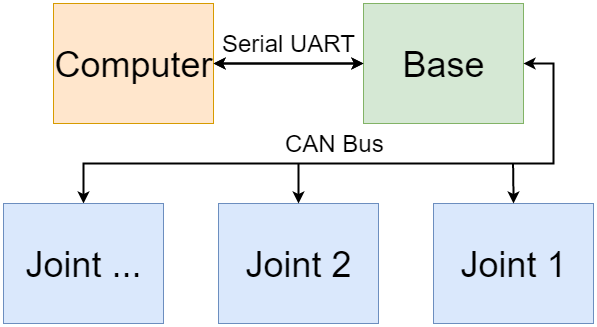
\includegraphics[scale=0.4]{system_coms_diagram}
	\caption{Block diagram of the entire modular arm system}
	\label{fig:system_block_diagram}
\end{figure}


\subsection{Fourth Joint and Existing Arm}
%TODO: insert solidworks .dwg files and place them in the correct spot
In order to show that our control system can be integrated with other arms, we designed a fourth joint to connect to an existing arm. By showing that we can add a newly designed joint to our existing arm, we are creating a proof-of-concept that shows the versatility of our control system.  The design of the fourth joint was done in Solidworks, a software that allows users to design objects in a 3-D space \cite{Solidworks}. Once we had designed the fourth link, we moved forward to the rapid-prototyping stage where we took our parts designed in Solidworks and converted them to 3-D printable models.  We then used the software Cura \cite{Cura} and the Lulzbot Taz 6 3-D printer \cite{Taz6} to fabricate a first iteration of our fourth joint.  From here we continued to refine our parts and re-print pieces with tighter tolerances until they came together to make a fourth joint that interfaces with our control system.

\subsubsection{Fourth Joint Design}
The process of prototyping our fourth joint started with creating an interface so that we can connect it to the already existing arm.  We decided for the sake of simplicity to attach our fourth joint where the current end-of-arm-tooling would normally connect. \\

\begin{figure}[H]
	\centering
	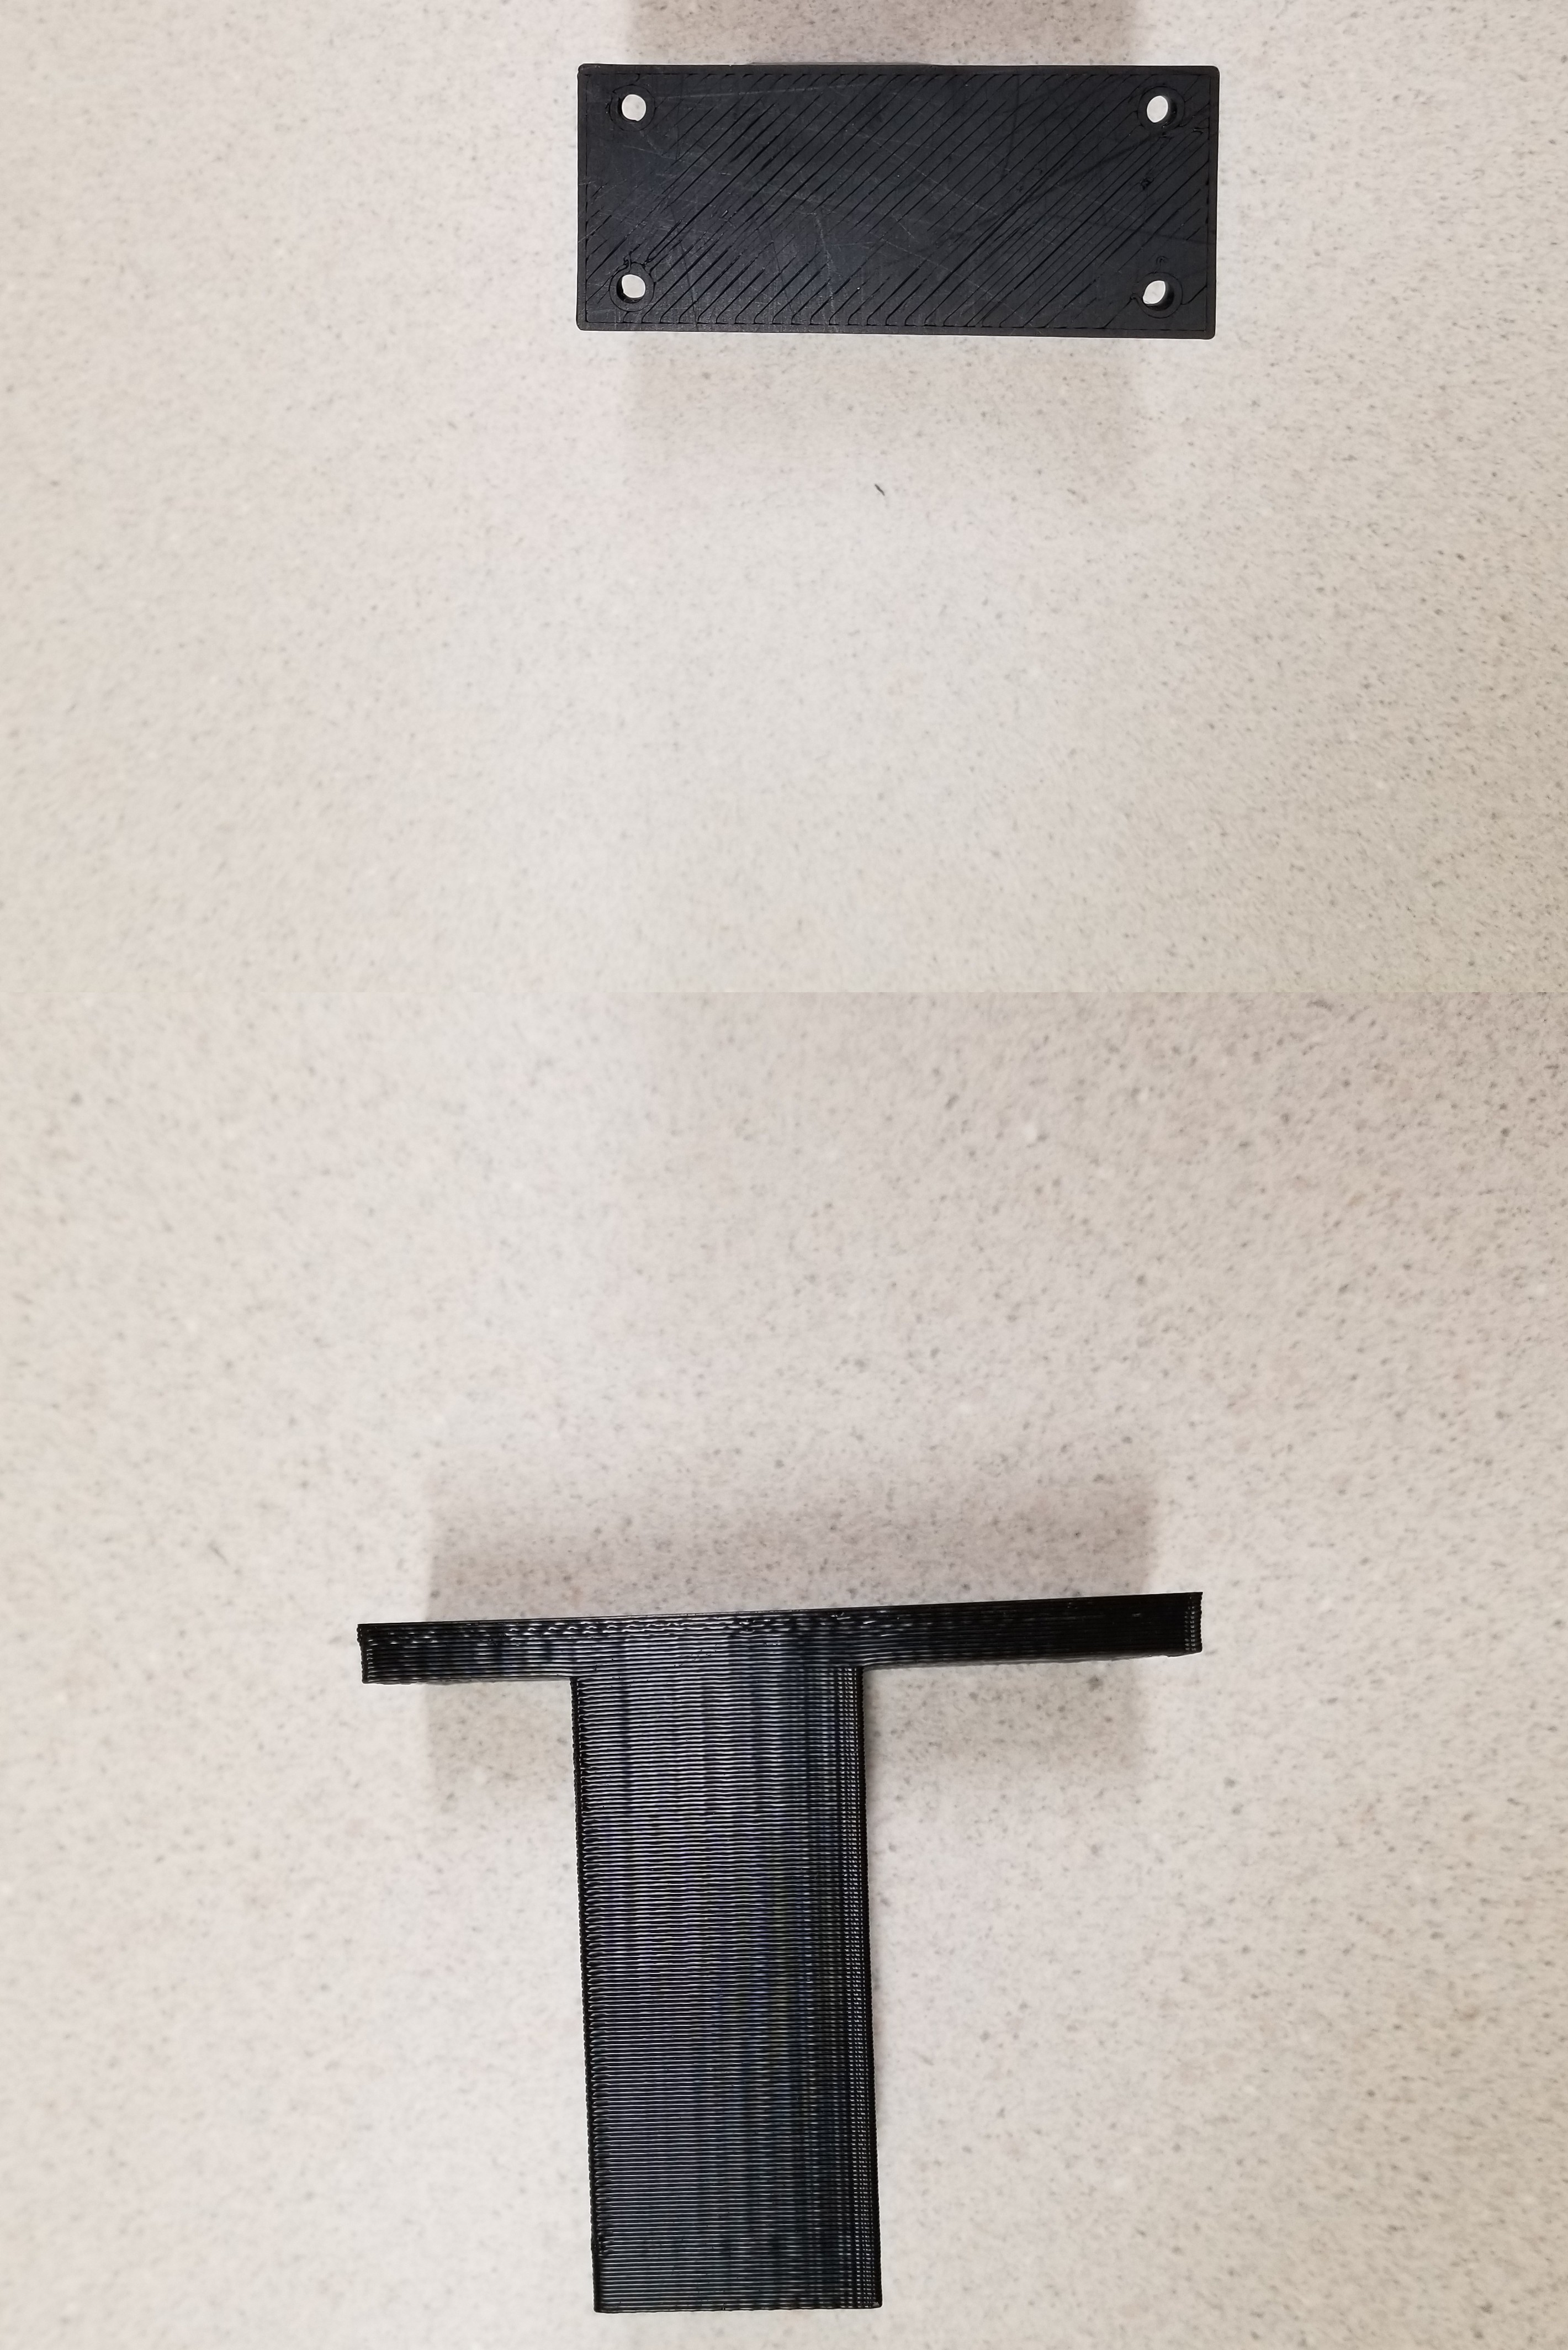
\includegraphics[angle=90, scale=0.1]{current_arm_connector}
	\caption{Current Arm End Effector Mount}
	\label{Current Arm Encoder Mount}
\end{figure}

\begin{figure}[H]
	\centering
	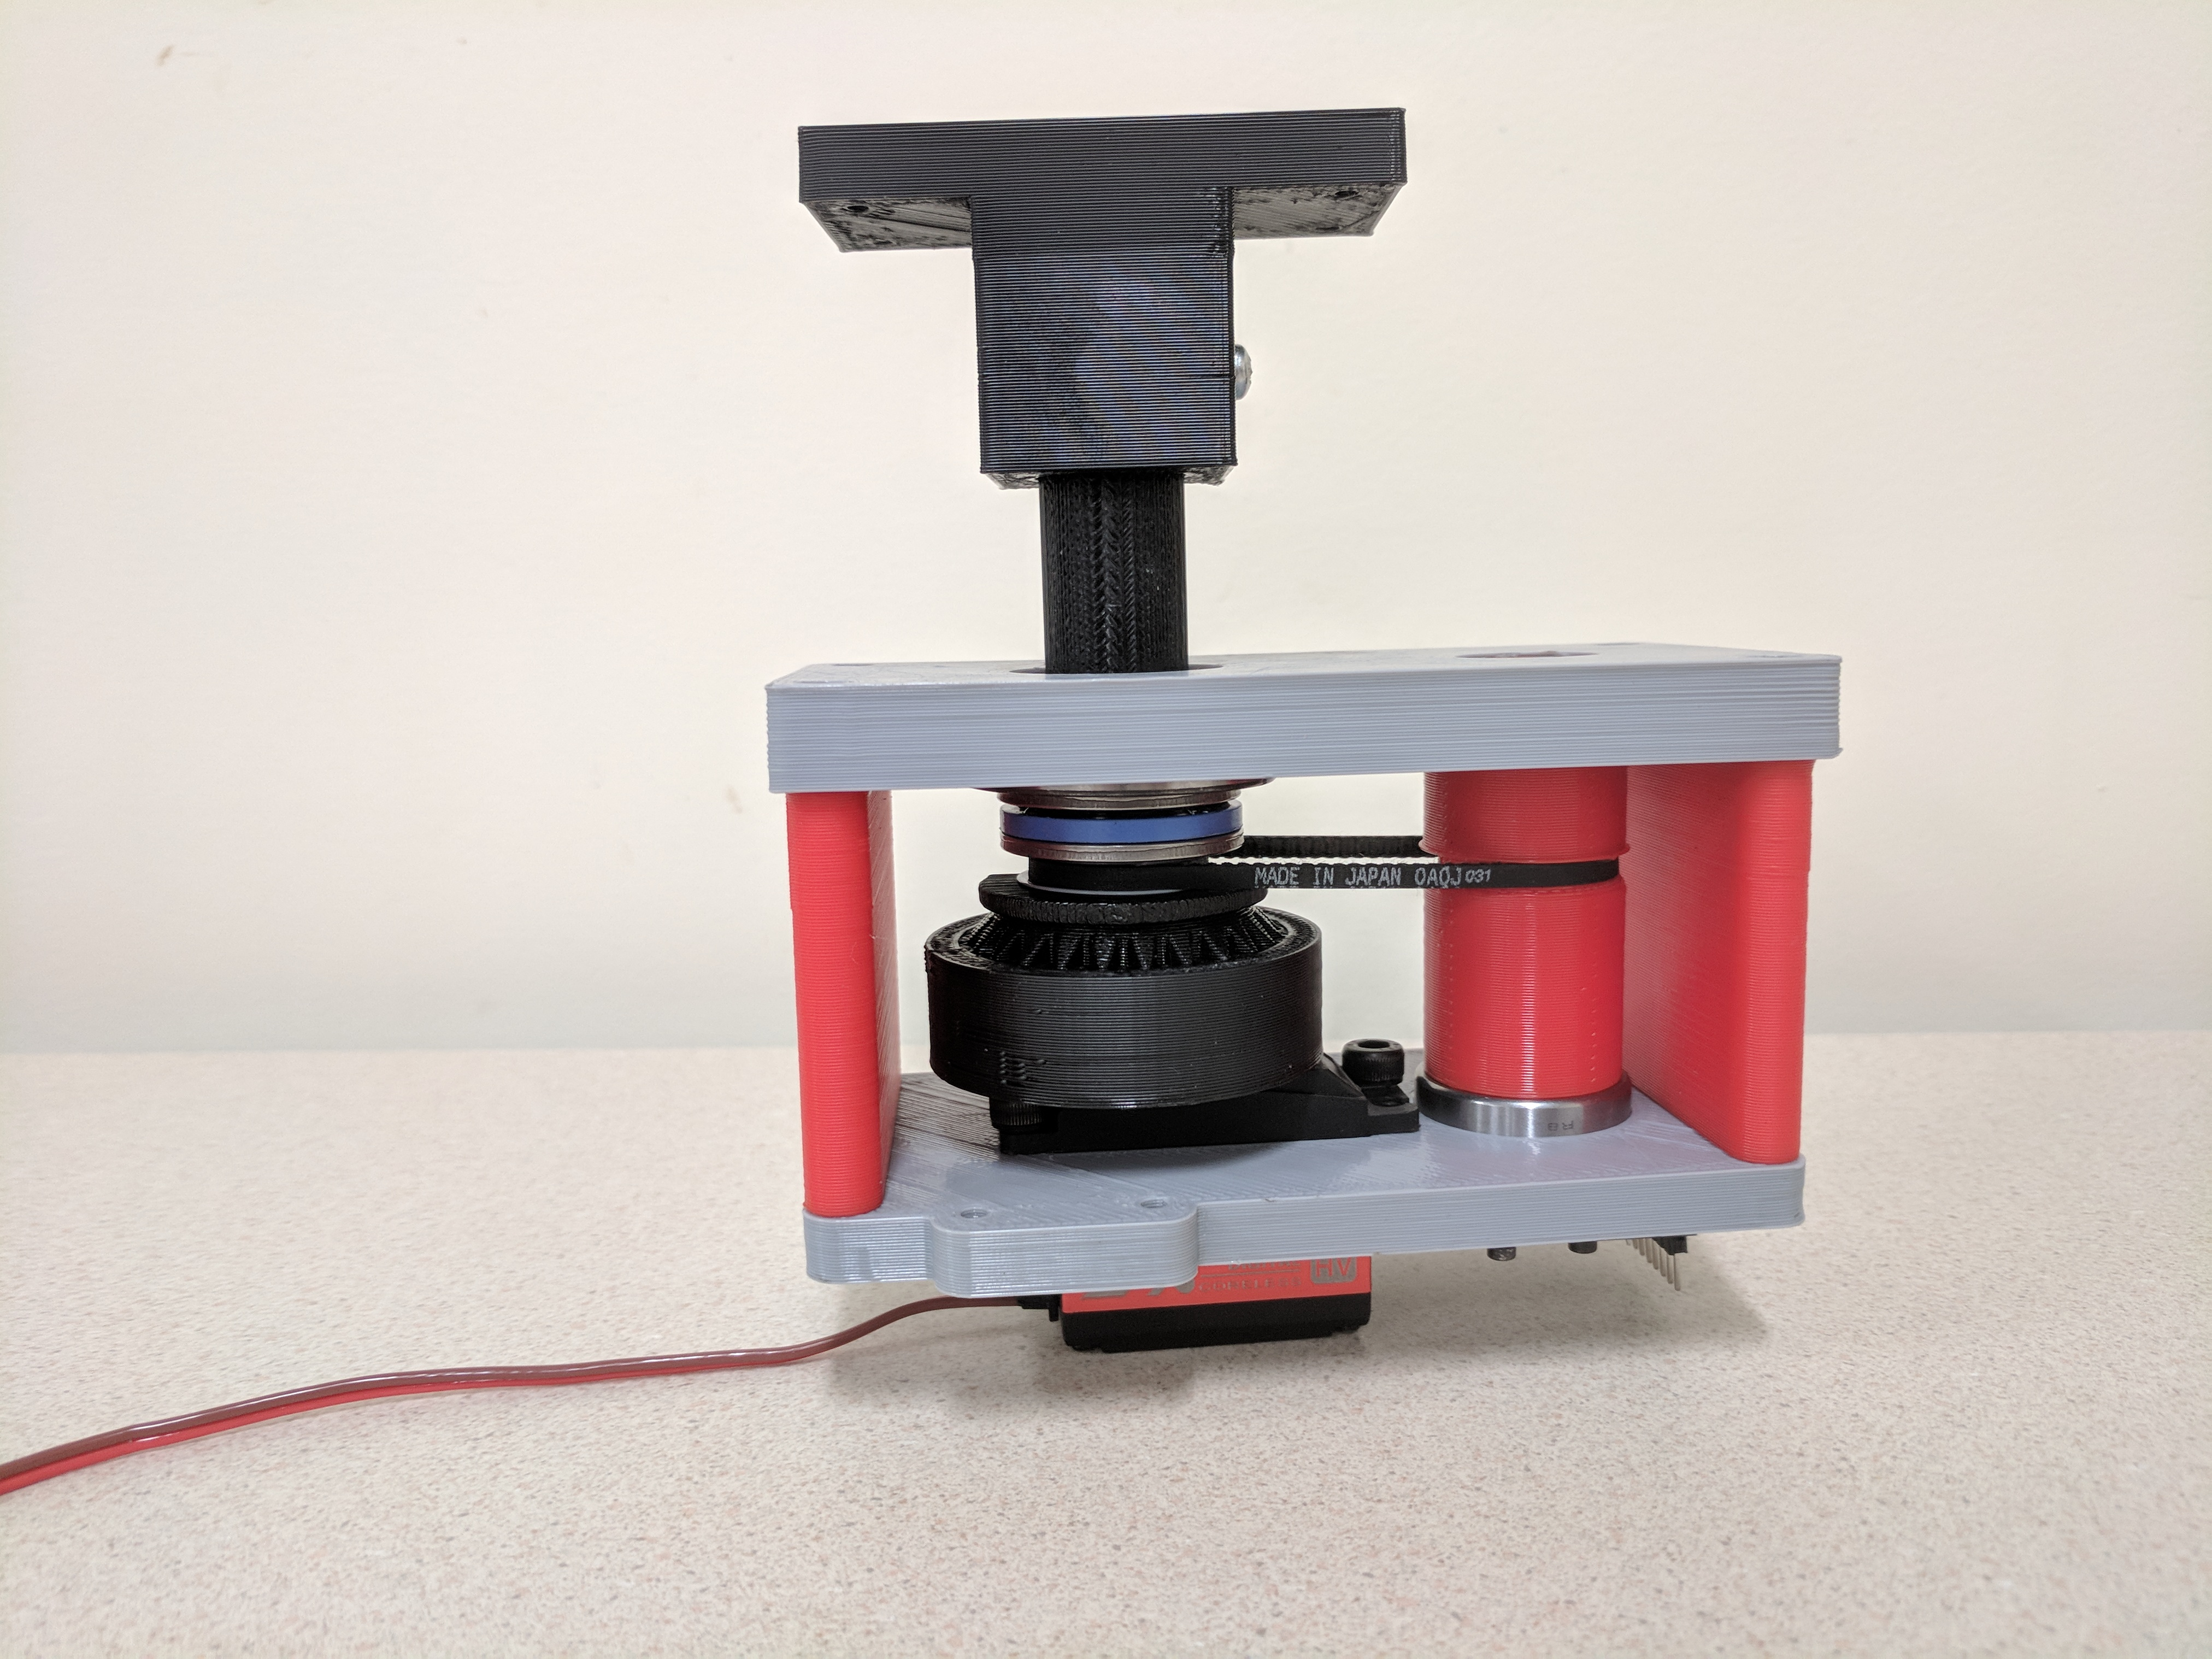
\includegraphics[scale=0.07]{Joint_4_Side}
	\caption{Side View of Final Removable Joint}
	\label{fig:Side View of Joint 4}
\end{figure}

\noindent Our second decision was to create a joint that is actuated using a brushed DC motor to prove that we can control DC motors in addition to the servos that already exist on the arm.  Next, we decided that since most of the joints currently on the arm provide rotation perpendicular to the z-axis of the actuator, we wanted a joint that provides parallel rotation. To accomplish this we removed the control logic from a servo that already was used on the arm, converting it into a brushed DC motor. Next, we designed a direct-drive mount for the motor we fabricated so that the output shaft would rotate along the motor's axis of rotation.  We built a mounting for the motor and a structure to provide support for both radial and axial load on the shaft. This structure made use of multiple radial bearings, placed to keep the shaft in line and eliminate any friction between moving and static pieces of the joint.  We also included a thrust bearing on the main shaft in order to stop thrust loads from being placed directly on the servo.  Finally, we designed an idler-shaft that sits in two bearings so that it can free rotate with negligible friction. The purpose of this idler shaft is to rotate in a 1:1 gear ratio with the main shaft using a timing belt to connect the two shafts.  At the bottom of the idler shaft there is a magnet whose changing magnetic field is read by a Hall effect sensor mounted onto the bottom of the fourth joint so that it sits exactly 1mm from the magnet, allowing for optimal position reading.  \\

\subsubsection{Fourth Joint Prototyping}
The process of prototyping our fourth joint started with creating an interface so that we can connect it to the already existing arm.  We decided for the sake of simplicity to attach our fourth joint where the current end-of-arm-tooling would normally connect. %TODO: MOVE UP

\noindent To create a prototype of our fourth joint, we determined the mechanical requirements of our arm and worked backwards to create a rapid prototyping model (RPM).  RPMs are usually CAD models which are able to be turned into a functional model using a 3-D printer. or other method.  Once the functional model was 3-D printed, we would assemble the parts and test how they all fit together.  With each new functional model we revised our RPM and printed a new functional model in order to meet the requirements for our fourth joint. This process of building, revising based on testing a physical prototype was only made possible due to the advances in recent years in 3-D printing technology making it feasible to create these prototypes so quickly while still having them be robust. 

\subsubsection{3-D Printing}
3-D printing is convenient because it allows the user to manufacture parts in a novel way. Overall, we chose to 3-D print our fourth joint because it was what we were most familiar with and we had easy access to multiple 3-D printers.  While the process of 3-D printing a part might not be as accurate as other more conventional methods of machining parts, it is a much easier method to learn and has a much quicker turnaround time. For our choice of 3-D printer, we used the LulzBot Taz 6 \cite{Taz6} with a single extruder head (Version 2.1) and 2.65mm filament. This printer is readily available to us through the Undergraduate Robotics Lab. The resolution of the printer was fine enough that it was easily able to achieve the tight tolerances that we needed to print parts such as the timing belt teeth.  

%TODO: Those pretty calculations from Chris's notebook that show that the small part won't be crushed

\subsubsection{Motor Selection}

The performance of a DC motor can be characterized by measuring several key values: the stall torque, the stall current, the free running RPM, and the free running current. It's important that all the values be measured when the motor is given the same input voltage.\\

\noindent
Specifications:\\
\noindent
\indent Voltage: 8.4V \\
\indent Stall torque: 32.3 kg cm stall \\
\indent Stall current: 5.25 A stall \\
\indent Free running RPM: 0.1 seconds/60 degrees (100 rpm) \\
\indent Free running current: 0.23 A \\





\begin{table} [H]
	\centering
	\caption{HV5923MG Motor Curve Data from experimental testing}
	\label{tab:MotorData}
	\begin{tabular}{|p{1cm}|p{1.2cm}|p{1.4cm}|p{1cm}|p{1cm}|p{1.5cm}|p{1cm}|p{1cm}|p{1.1cm}|}
		\hline
		Speed (RPM) & Torque (N-m) & Torque (in-lbf) & Current (A) & $P_{out}$ (W) & Efficiency (\%) & $P_{in}$ (W) & Heat (W) & back-EMF (V) \\
		\hline
		
		0 & 3.16 & 27.98 & 5.25 & 0 & 0 & 44.1 & 44.1 & 0 \\
		
		7 & 2.94 & 26.02 & 4.9 & 2.15 & 5.24 & 41.15 & 38.99 & 0.56 \\
		
		13 & 2.75 & 24.34 & 4.6 & 3.74 & 9.69 & 38.62 & 34.87 & 1.04 \\
		
		20 & 2.53 & 22.38 & 4.25 & 5.3 & 14.85 & 35.67 & 30.37 & 1.61 \\
		
		27 & 2.31 & 20.42 & 3.89 & 6.52 & 19.94 & 32.71 & 26.19 & 2.17 \\
		
		33 & 2.12 & 18.74 & 3.59 & 7.32 & 24.24 & 30.18 & 22.87 & 2.65 \\
		
		40 & 1.9 & 16.79 & 3.24 & 7.94 & 29.17 & 27.23 & 19.29 & 3.21 \\
		
		47 & 1.68 & 14.83 & 2.89 & 8.24 & 33.96 & 24.28 & 16.04 & 3.78 \\
		
		53 & 1.49 & 13.15 & 2.59 & 8.24 & 37.9 & 21.75 & 13.51 & 4.26 \\
		
		60 & 1.26 & 11.19 & 2.24 & 7.94 & 42.25 & 18.8 & 10.86 & 4.82 \\
		
		67 & 1.04 & 9.23 & 1.89 & 7.32 & 46.18 & 15.85 & 8.53 & 5.38 \\
		
		73 & 0.85 & 7.55 & 1.59 & 6.52 & 48.99 & 13.32 & 6.79 & 5.86 \\
		
		80 & 0.63 & 5.6 & 1.23 & 5.3 & 51.09 & 10.37 & 5.07 & 6.43 \\
		
		87 & 0.41 & 3.64 & 0.88 & 3.74 & 50.49 & 7.41 & 3.67 & 6.99 \\
		
		93 & 0.22 & 1.96 & 0.58 & 2.15 & 44.12 & 4.88 & 2.73 & 7.47 \\
		
		100 & 0 & 0 & 0.23 & 0 & 0 & 1.93 & 1.93 & 8.03 \\
		\hline
		
	\end{tabular}
	
\end{table}

\begin{figure}[H]
	\centering
	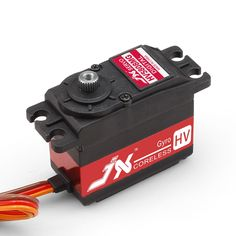
\includegraphics{motor}
	\caption{HV5923MG Servo Motor}
	\label{fig:HV5923MG Servo Motor}
\end{figure}


\subsubsection{Arm Base}
% Talk about requirements for base
% take in new joint data at certain speeds
% output new joint data at certain speeds
The mechanical side of the base module is relatively simple because the physical structure comes from the pre-existing arm. In order to make this compatible with our controls system, all we have to do is mount our joint and encoder boards to it. This is fairly simple since we use a slightly modified version of the encoder board on the existing arm with the same mounting scheme. Our joint board mounting scheme focused around mounting each board in a place where it would not be impeded by the movement of the arm during runtime. 

\begin{figure}[H]
	\centering
	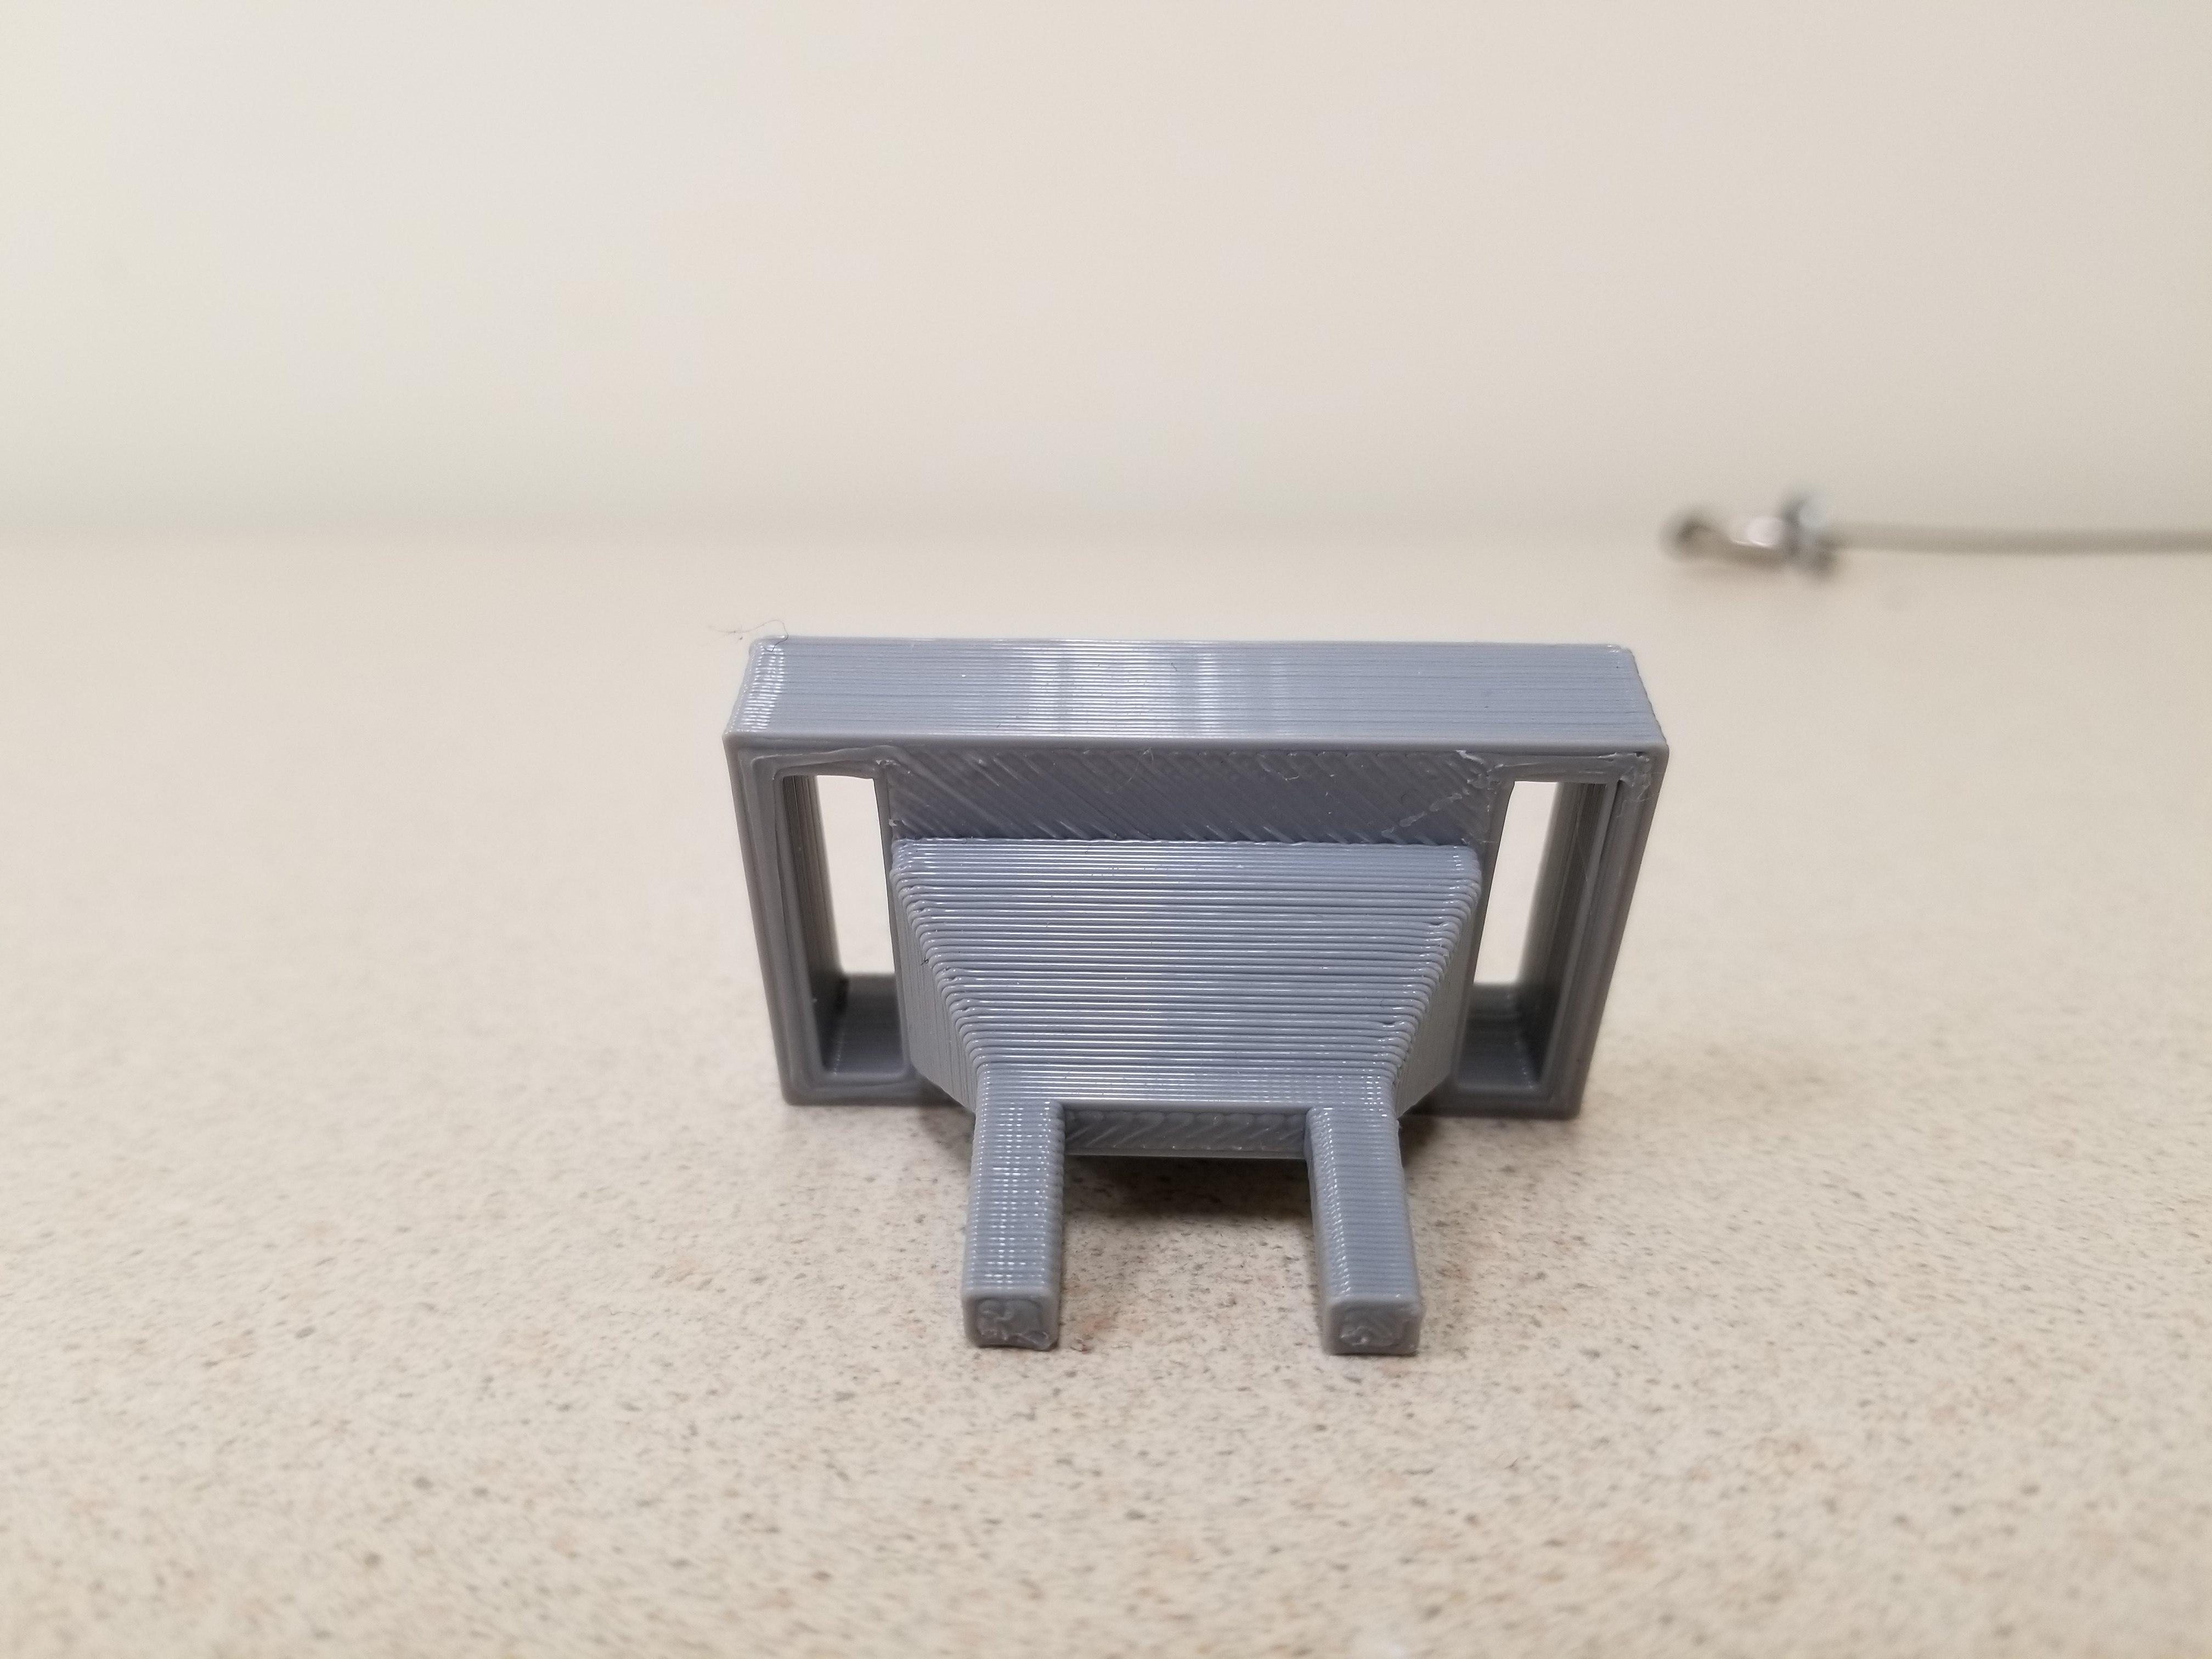
\includegraphics[width=\textwidth]{mount_back_view}
	\caption{TM4C123G to arm mount}
	\label{fig:mount_back_view}
\end{figure}

\begin{figure}[H]
	\centering
	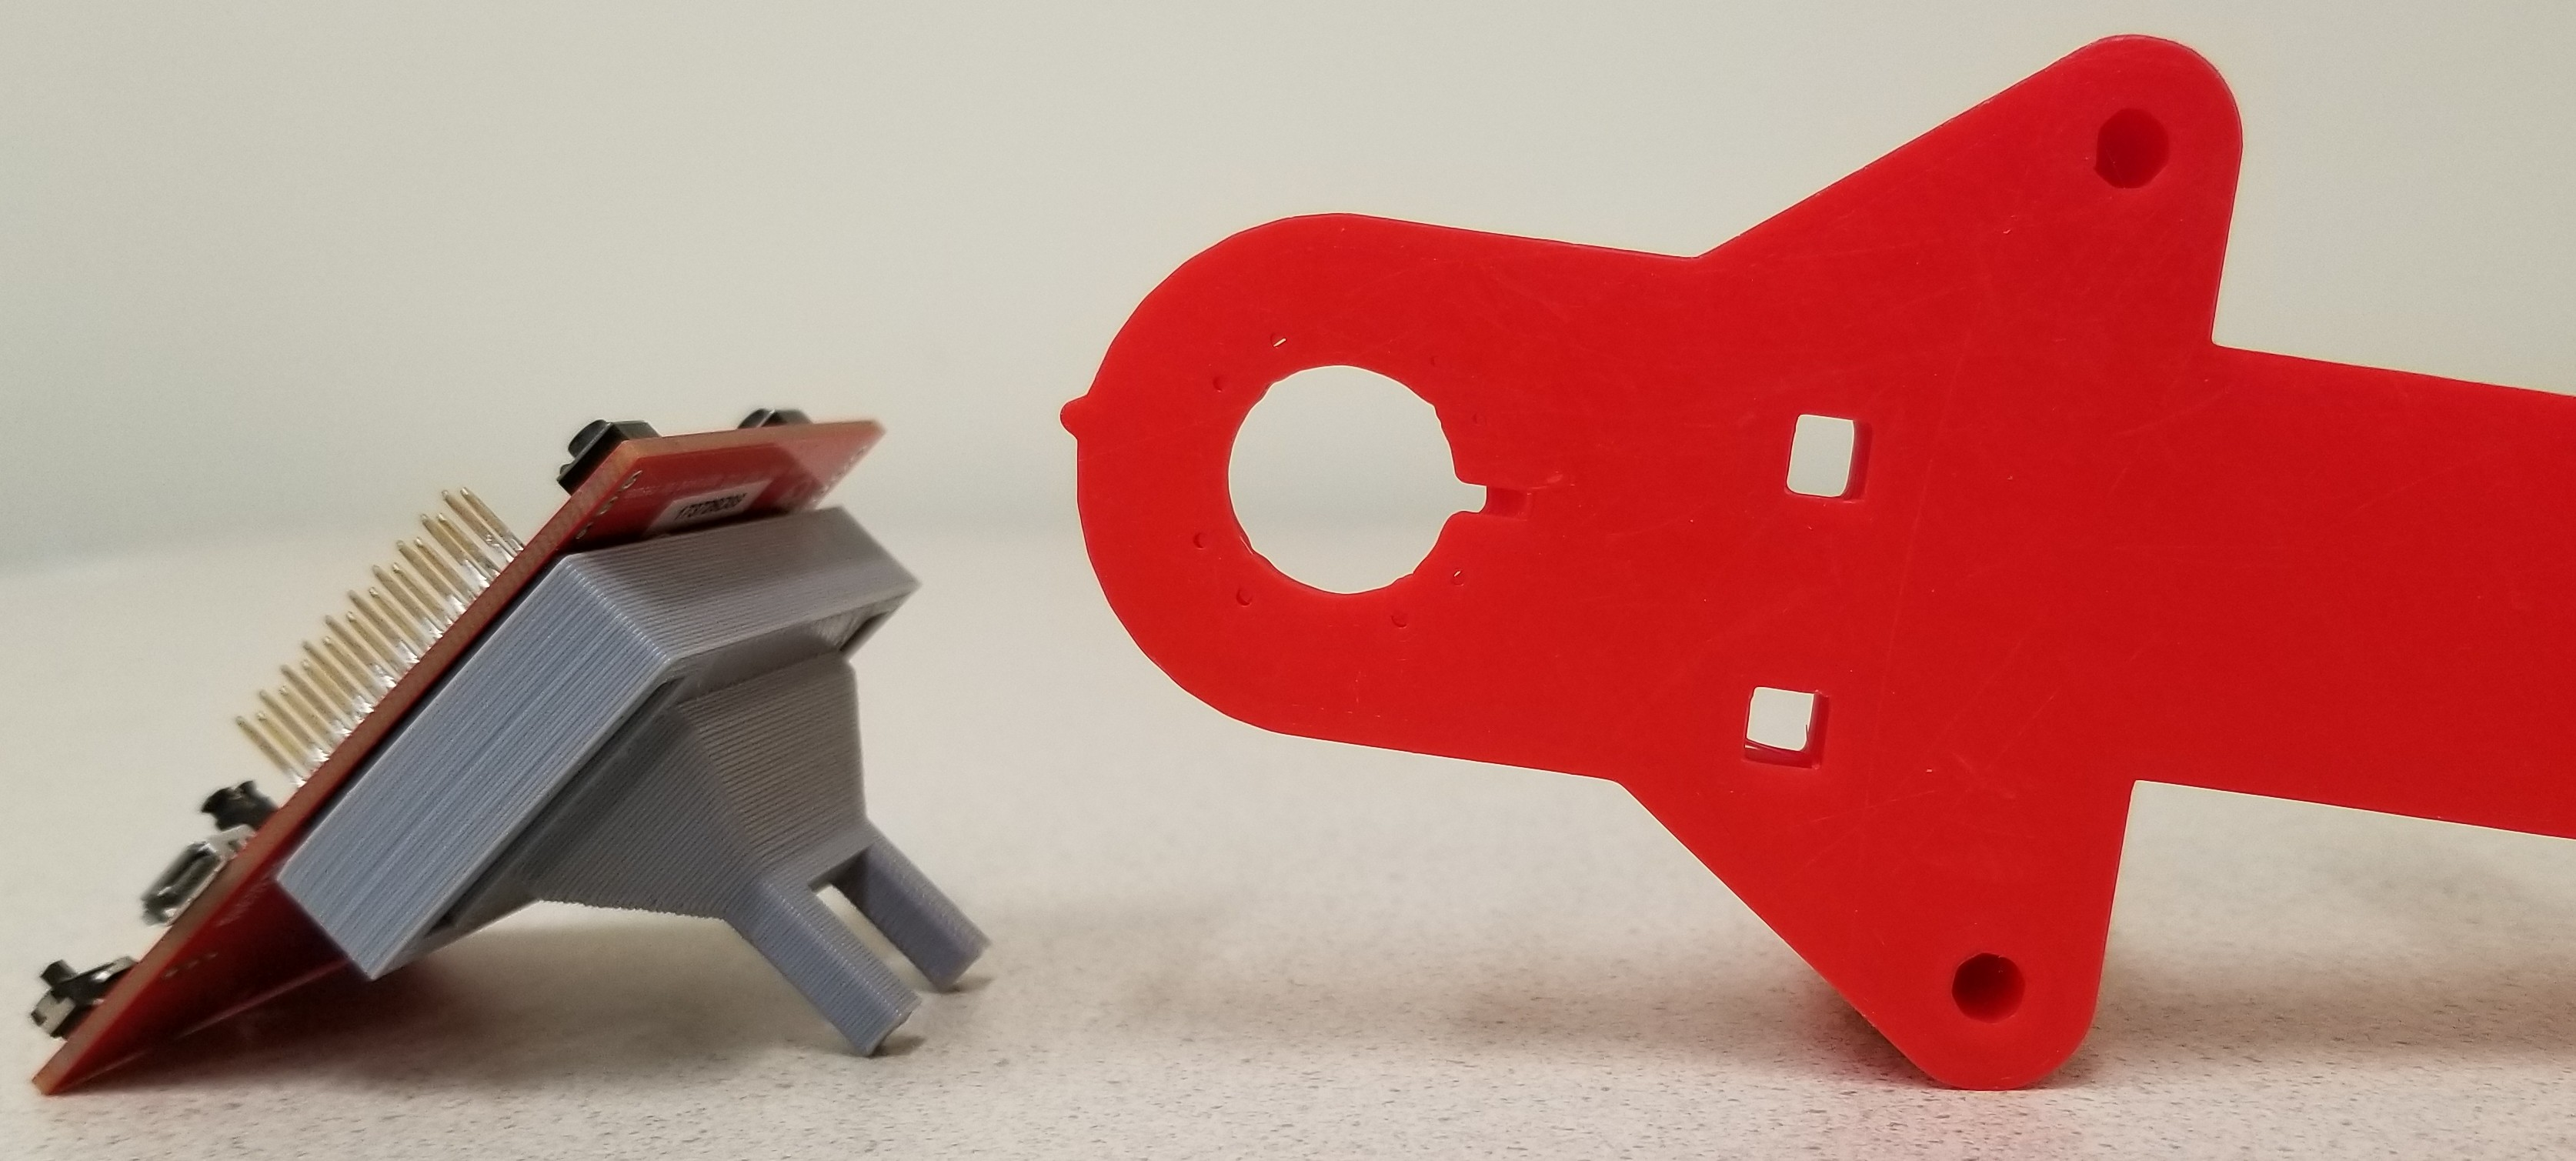
\includegraphics[width=\textwidth]{mount_and_holes}
	\caption{Mounting holes on arm and mounted TM4C123G}
	\label{fig:mount_and_holes}
\end{figure}

\noindent We have not only made sure that none of the mechanical components of the arm would come into contact with the board but also that none of the wiring between boards would be unplugged. This meant that we had to mount the boards far enough away from moving parts while still keeping it close enough to the sensors and motors that needed to interface with it. We decided to mount it in the same position for each category of joint type to keeps these needs consistent. Making use of an already existing area used to mount the cabling for the previous iteration of the arm seemed like the most efficient way to go about this. We designed a mechanical interface that was able to press-fit into our joint board and connect to the previous mounting solution.


\subsection{Joint Control Board}
The joint control board sits at the heart of the entire functionality of the project. Without a robust and capable design, any arm constructed would not function properly. Selecting the types of sensors to use for the control board was a very important step of the joint control board design. %todo FINISH THISS

\subsubsection{Overview of Design}
The joint board underwent significant revisions, outlined in Section \ref{sec:pjcbd}, but the depth of revision significantly dropped after the decision was made to use the TM4C123GH6PM 32-bit ARM processor. This processor had many peripherals internally that simplified the joint board design significantly. A block diagram of the final joint control board can be seen in Figure \ref{fig:jcb_block_diagram}.

\begin{figure}[H]
	\centering
	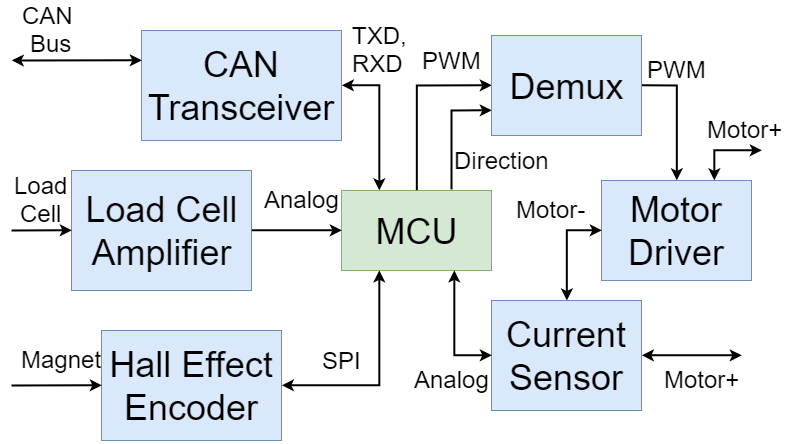
\includegraphics[scale=0.4]{jcb_block_diagram}
	\caption{Block diagram of the joint control board}
	\label{fig:jcb_block_diagram}
\end{figure}

\subsubsection{Joint Angle Sensor}
\label{sec:jas}
Potentiometers seem like a good choice due to their simplicity and high accuracy capabilities. However, they do not lend themselves well to this application because of how quickly they wear out. Over time, as the joints move to different positions, the potentiometers will wear out quickly and cause inaccurate readings. Additionally, long lifespan and high resolution potentiometers can be very expensive. Furthermore, potentiometers are large and can be difficult to mount. Finally, the hard stop on the potentiometer means the joint angles will be limited to a certain range (typically about 270 \textdegree for single turn potentiometers).

\noindent The next obvious solution is to use optical encoders because they will not wear out and offer very high resolution capabilities. These sensors are not well suited for this application, however, since they are typically expensive, especially for high resolution encoders - and ones that are capable of reading absolute position. Additionally these sensors are somewhat bulky and would take up too much space in the closed environment of a joint. 

\noindent This leaves us with Hall effect sensors. These sensors are very small and moderately high resolution while also being a contact-free sensor, so wearing them out will not be a concern. A main concern with Hall effect sensors is that they need to be mounted somewhat precisely and carefully. Traditional machining methods make this difficult to accomplish, but 3D printing allows us to easily overcome this challenge.  Another concern is external electromagnetic interference, but with somewhat careful circuit board design, we should be able to minimize this issue.

\subsubsection{Motor Current Sensor}
A shunt resistor seems practical due to the simplicity of the design, but careful tuning must be done in order to get the noise levels down to a reasonable amount. In addition to this, the power loss when using a shunt resistor could cause the arm to stall before anticipated. When the shunt resistor takes power from the motor, the whole motor curve slides inward, decreasing the maximum power output. Trace resistance would be a good alternative, but requires calibration after the circuit is constructed. 

\noindent Instead of these, we decided to use a Hall effect current sensor. Hall effect current sensors are ready-made sensors that give low noise, properly calibrated outputs, are not very expensive, and are easy to integrate into a circuit design. These sensors have extremely small power losses to the motor. The main drawback of these sensors is that they have a low bandwidth, but we are using DC motors so this should not be a problem. Some care will need to be taken when placing these on the circuit, however, since they are sensitive to external magnetic fields.

\begin{table}[H]
	\centering
	\caption{Current Sense IC Comparison}
	\begin{tabular}{|p{4.2cm}|p{1.5cm}|p{2cm}|p{1.7cm}|c|p{1.4cm}|}
\hline
Part name & Supply Voltage (V) & Current Range (A) & Sensitivity (mV/A) & Output & Built in filter? \\
\hline

ACS722LLCTR-05AB & 3.3 & -5 to +5 & 264 & Analog & y \\

ACS723LLCTR-05AB & 5 & -5 to +5 & 400 & Analog & y \\

ACS724LLCTR-10AB & 5 & -10 to +10 & 200 & Analog & n \\

ACS725LLCTR-10AU & 3.3 & 0 to +10 & 264 & Analog & n \\
\hline

\end{tabular}

	\label{tbl:Current Sense IC Comparison}
\end{table}

\subsubsection{Inter-board Communication}
SPI and I$^2$C are mostly used for on-board, controller-to-peripheral communications and therefore are not a good choice for the base to control board communication. RS232 is not a good solution for this problem either because it is a single transmitter and single receiver per line. This leaves RS485 and CAN.

\noindent RS485 and CAN are similar in many ways, but with a few key differences that separate them. RS485 is very fast to transmit and simple to implement, but takes a lot of the controller's time to send packets. CAN has the advantage because the controller and transceiver control the transmission independent of the controller so the controller has more free time to process data. Another advantage CAN has over RS485 is the amount of error checking that goes on to ensure proper message transmission. For these reasons, we decided to use CAN to communicate between the base and control boards.

\subsubsection{Preliminary Joint Control Board Designs}
\label{sec:pjcbd}
Preliminary joint control board design was done very early on in the project. Unfortunately, the majority of this work was done before much of the necessary research for part selection, leading to many revisions and re-designs, though the main concepts stayed in place. This section outlines the preliminary designs and revisions of those up until the selection of the TM4C123GH6PM microcontroller, at which point the design solidified and forward progress began. 

\begin{figure}[H]
	\centering
	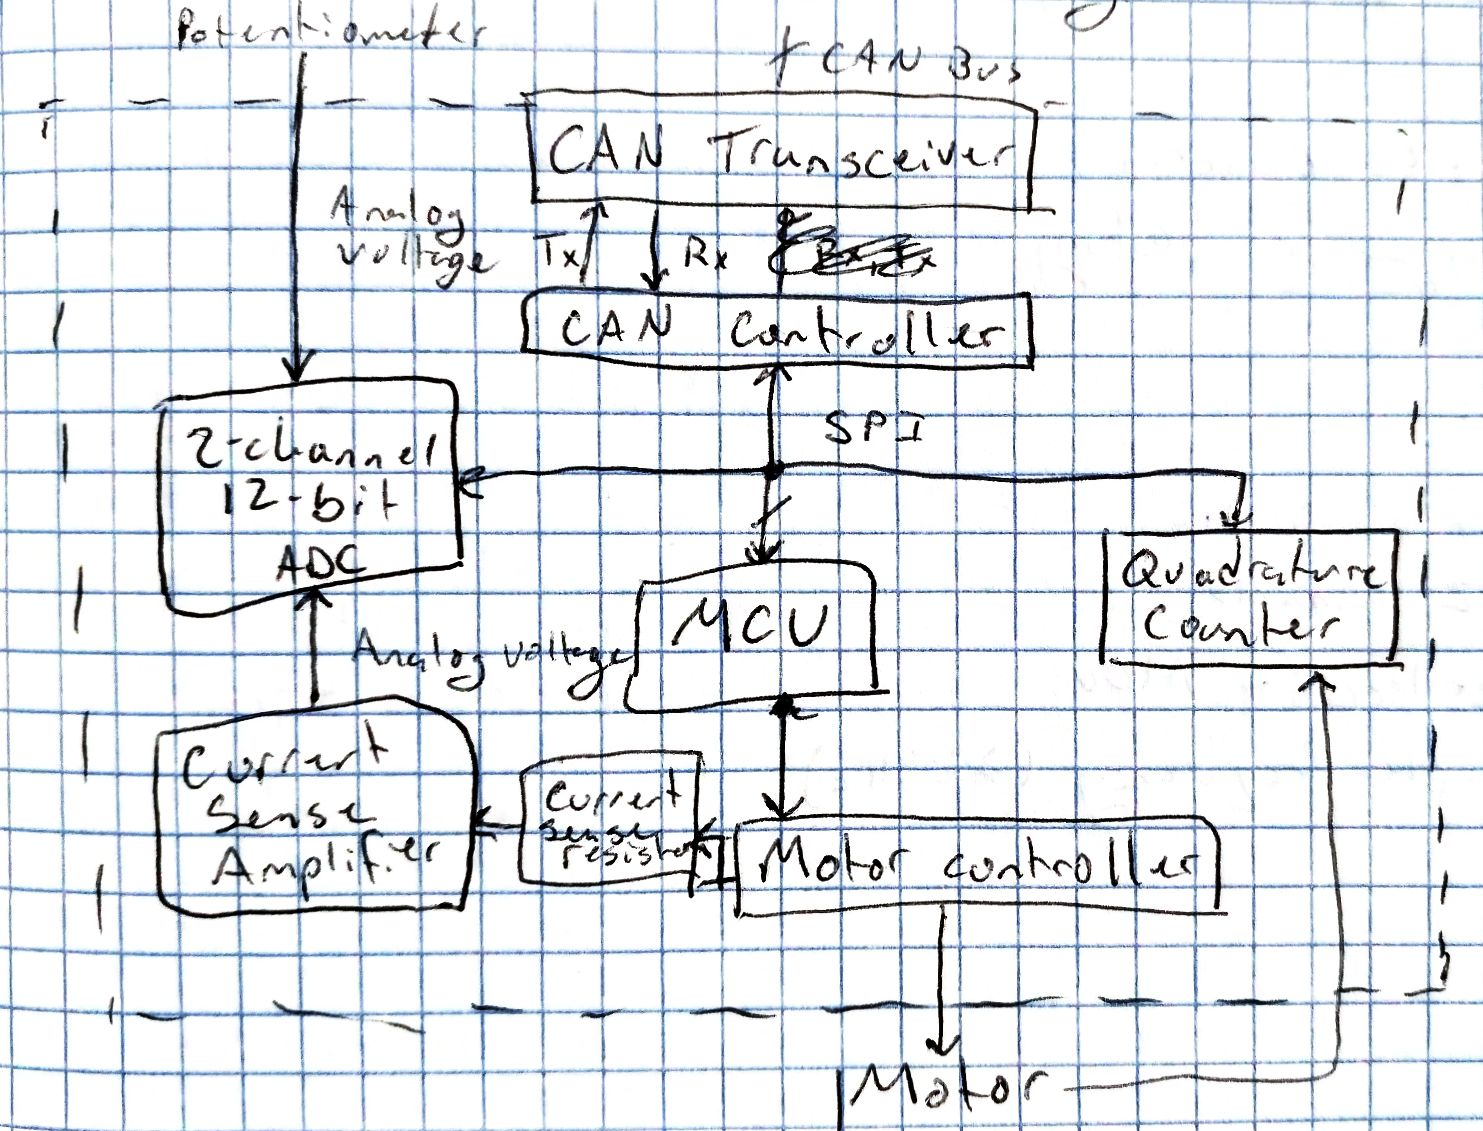
\includegraphics[scale=0.18]{first_joint_board_block_diagram}
	\caption{First draft of the complete joint board block diagram}
	\label{fig:1st_joint_board_block}
\end{figure}

\noindent The first complete block diagram of the joint control board Figure \ref{fig:1st_joint_board_block}. This diagram was centered around a MSP430G series microcontroller, and focused on keeping the cost of the board down. Some component selection was solidified , including the following: MSP430G2553 (microcontroller), MCP3202 (ADC), DRV8872 (motor driver), LS7366R (quadrature counter), MCP2515 (CAN controller), and MCP2561 (CAN transceiver). 

\noindent The decision to replace the potentiometer with an absolute hall effect encoder was made to lengthen the lifespan of the device. Greater detail about this decision is presented in Section \ref{sec:jas}. This change resulted in the diagram shown in Figure \ref{fig:nice_prelim_joint_board_block}. Certain components, such as the CAN controller and transceiver, operated at 5V while others, such as the microcontroller and absolute hall effect encoder, required 3.3V. Most other components could function at either voltage, and were placed on either side of the level shifter for other reasons. The ADC, for example had a supply-voltage-dependent maximum SCLK frequency.
\begin{figure}[H]
	\centering
	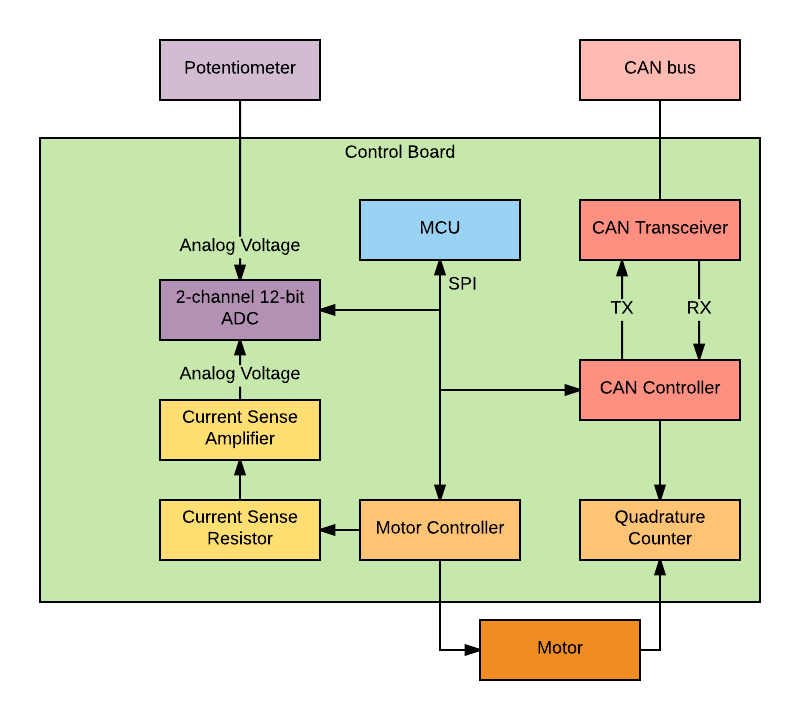
\includegraphics[scale=0.3]{link_block_diagram}
	\caption{Iteration of preliminary joint board block diagram}
	\label{fig:nice_prelim_joint_board_block}
\end{figure}

\noindent Some planning was done to coordinate communication between the components, including placement of a 3.3V to 5V level shifter. This planning led to the block diagram shown in Figure \ref{fig:2nd_joint_board_block}. This diagram requires many lines to pass through the level shifter, which is not ideal and led to the decision to revise component selection.

\begin{figure}[H]
	\centering
	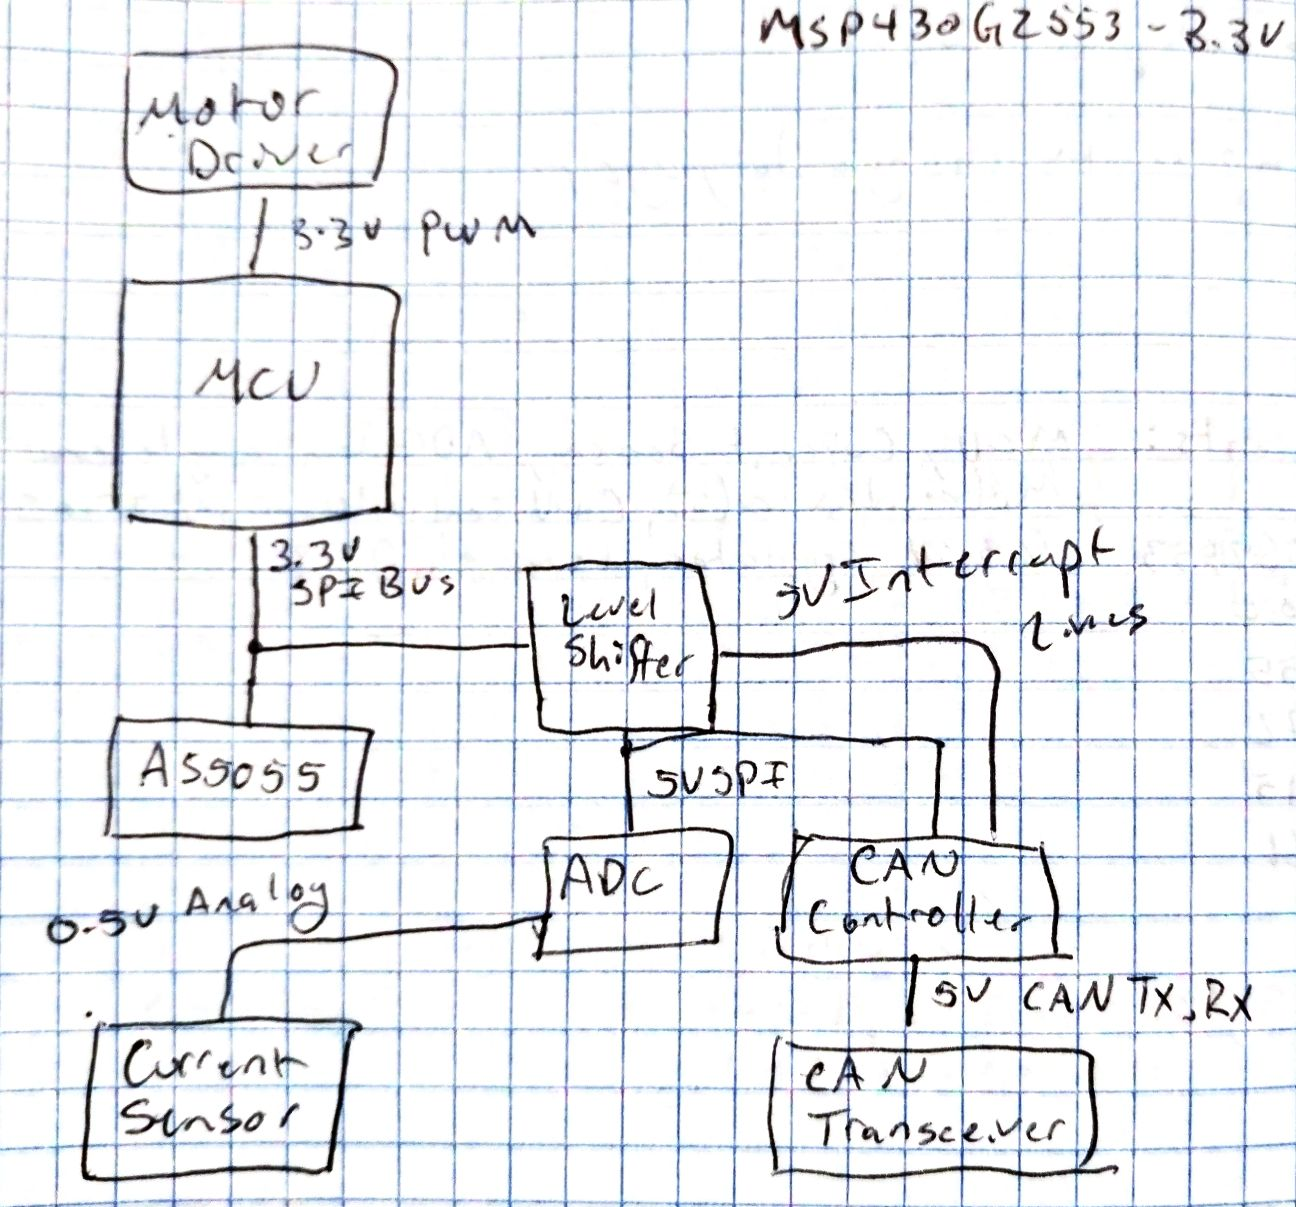
\includegraphics[scale=0.2]{second_joint_board_block_diagram}
	\caption{Mostly complete preliminary joint board block diagram}
	\label{fig:2nd_joint_board_block}
\end{figure}

\subsubsection{ADC Selection}
The first design of the joint control board used a potentiometer to detect the joint angle and a current sense amplifier to detect the motor current. Both of these signals require an ADC to process, and the original microcontroller did not have a high resolution ADC on board, so an off board ADC was needed. Table \ref{tbl:ADC Selection} highlights the different ADCs that were evaluated before selecting one. The MCP3202, while not necessarily the best option from the chart, was selected since it has a very easy to use interface and was available in DIP package for easy testing. With the switch from the MSP430G2553 to the TM4C123GH6PM, the external ADC was no longer needed.

\begin{table}[H]
	\centering
	\caption{ADC Selection}
	
	\begin{tabular}{|c|c|c|c|c|}
		\hline
		& Supply & Sampling & SCLK & \\
		Part name & Voltage (V) & rate (MHz) & Freq (MHz) & Price (\$) \\
		\hline
		ADS7042 & 3.3 & 1 & 16 & 2.65 \\
		
		ADS7043 & 3.3 & 1 & 16 & 2.65 \\
		
		ADS7044 & 3.3 & 1 & 16 & 2.65 \\
		
		ADC121S021 & 3.3, 5 & 0.2 & 4 & 2.85 \\
		
		ADC121S051 & 3.3, 5 & 0.5 & 4 & 3.31 \\
		
		ADC121S101 & 3.3, 5 & 1 & 4 & 3.39 \\
		
		ADC7476 & 3.3, 5 & 1 & 20 & 3.41 \\
		
		MCP3202 & 3.3, 5 & 0.1 & 1.6 & 2.31 \\
		
		MAX11665 & 3.3 & 0.5 & 8 & 2.73 \\
		\hline
	\end{tabular}
	
	\label{tbl:ADC Selection}
\end{table}

\subsubsection{Preliminary Price Breakdown}
Initially, one of the goals of this project was to produce a very low cost joint board. An estimate that matches the joint board block diagram from Figure \ref{fig:nice_prelim_joint_board_block} can be seen in Table \ref{tbl:Summary of Parts Selection}.
\begin{table}[H]
\centering
\caption{Summary of Parts Selection}

\begin{tabular}{|c|c|c|c|}
	
	\hline
	Function & Part name & Price (qty: 1) & Price (qty: 1k) \\
	\hline
	
	CAN Controller & MCP2515 & \$1.87 & \$1.42 \\
	
	CAN Transceiver & MCP2561 & \$0.90 & \$0.68 \\
	
	ADC & MCP3202 & \$2.61 & \$1.98 \\
	
	MCU & MSP430G2553 & \$2.41 & \$1.18 \\
	
	Motor Controller & DRV8872 & \$2.17 & \$1.06 \\
	
	3.3V Voltage Regulator & LP2950-33 & \$0.47 & \$0.13 \\
	
	Current Sensor & ACS723LLC10AB & \$5.53 & \$2.36 \\
	
	Encoder & AS5055a & \$8.07 & \$5.48 \\
	\hline
	\hline
	Price (qty: 1) & \$24.03 & & \\
	
	Price (qty: 1k) & \$14.30 & & \\
	\hline
	
\end{tabular}

\label{tbl:Summary of Parts Selection}
\end{table}	

\subsubsection{Motor Driver}
The DC motor driver selected was the DRV8872. This driver takes in two inputs, in1 and in2, which affect the output much like inputs to an H-bridge.The exception is when both inputs are high. In this case, the inputs are pulled together as a motor break. A truth table can be seen in Table \ref{tbl:drv8872-truth6}.

\begin{table}[H]
	\centering
	\caption{DRV8872 truth table}
	\begin{tabular}{| c | c | c | c| c |}
		\hline
		IN1 & IN2 & OUT1 & OUT2 & Description \\
		\hline
		0 & 0 & Z & Z & Coast \\
		0 & 1 & L & H & Reverse \\
		1 & 0 & H & L & Forward \\
		1 & 1 & L & L & Brake \\
		\hline
	\end{tabular}
	\label{tbl:drv8872-truth6}
\end{table}

\noindent This motor driver was chosen because is provided high enough current limit for the selected motors to operate normally and low on resistance to provide more power to the motors and not generate excess heat. Another benefit of the DRV8872 is that it has a simple interface of 2 PWM inputs which is relatively easy to interface with from our microcontroller.
 
\begin{table}[H]
	\centering
	\caption{Motor Driver Comparison}
\begin{tabular}{|c|c|c|c|}
	\hline
	 & Peak & Continuous & \\
	Part name  & Current (A) & current (A) & Control method \\
	\hline
	
	LMD18245 & 6 & 3 & direction, brake \\
	
	DRV8842 & 6 & 3.5 & PWM \\
	
	DRV8829 & 5 & 3.5 & Phase, enable \\
	
	L298 & 3 & 2 & in1, in2, en \\
	
	DRV8872 & 3.6 & 3.5 & in1, in2 \\
	\hline
	\end{tabular}

	\label{tbl:Motor Driver Comparison}
\end{table}

\noindent To measure the speed of the motor, a servo horn with 6 spokes was attached and a beam break sensor was mounted on the motor with the spoke traveling through the beam. The signal line of the beam break sensor was connected to an Arduino that measured the frequency by incrementing a count in an interrupt triggered on a pin change. The ISR just incremented a count that was printed out and reset every 5 seconds. Some issues arose with this system, however, since there was a small amount of bouncing on the rising and falling edges, leading to multiple readings for each beam break. This was solved by placing a 10nF capacitor from the signal line to ground. Since this number was triggered 12 times per revolution and printed out every 5 seconds, the actual printed value happened to be in revolutions per minute, as shown in \ref{eqn:motor_driver_test}.

\begin{equation}
rpm = \frac{1 rev}{12 ticks} * \frac{1}{5} * \frac{60 seconds}{1 minute}
\label{eqn:motor_driver_test}
\end{equation}

\noindent During initial testing, the motor driver was wired up with $V_m$ of 8.4V, logic voltage of 5V, a 10k$\Omega$ pull up resistor on nFault, Isen grounded, and the motor outputs connected to a DC motor. During this test, one of the inputs was connected to an Arduino Uno, outputting a constant PWM wave using the \texttt{analogWrite()} function with a duty cycle of approximately 50\%. The motor turned, but very slowly and with a high pitched whine. When a 100$\mu$F capacitor was placed from $V_m$ to ground, the motor spun up to full speed and the whining sound went away.

\noindent Further testing revealed a strange behavior when increasing the frequency of the input PWM signal. The motor spun normally at low frequencies of around 500Hz, but at around 1kHz the motor started slowing down and making a whining sound. The problem worsened with increasing frequency. Eventually, this problem was fixed by using a power supply that could output 3A and adding capacitors from in1 and in2 to ground. With these additions, the motor driver functioned as expected.


\subsubsection{Demultiplexer}
A demultiplexer was not necessary for the operation of the joint board. However, it simplifies the motor control signal from two PWM lines to one PWM line and a digital output, speed and direction. Since it was fairly simple to implement, the additional complexity in the circuit was added and the software was simplified by only needing to set up a single channel on the PWM controller.

\noindent The original demultiplexer selected for the joint board (SN74LVC1G19) did not output the correct values to drive the motor driver (DRV8872). The demultiplexer output can be seen in Table  and the motor driver inputs can be seen in Table . When the EN pin was pulled high, both outputs would also be driven high. This effect is undesirable since, when given a PWM signal, this would cause the motor driver to turn then brake then turn again as opposed to the desired turn then coast then turn. To solve this problem, a different chip (SN74LVC1G18) was selected. The truth table for this chip can be seen in Table \ref{tbl:sn74lvc1g18-truth}.
\begin{table}[H]
	\centering
	\caption{SN74LVC1G18 truth table}
	\begin{tabular}{| c  c | c  c| }
		\hline
		\multicolumn{2}{|c|}{Inputs} & \multicolumn{2}{c|}{Outputs} \\
		\hline
		S & A & Y0 & Y1 \\
		\hline
		0 & 0 & L & Z \\
		0 & 1 & H & Z \\
		1 & 0 & Z & L \\
		1 & 1 & Z & H \\
		\hline
	\end{tabular}
	\label{tbl:sn74lvc1g18-truth}
\end{table}

\subsubsection{INA332}
\label{sec:meth-ina332}

\begin{figure}[H]
	\centering
	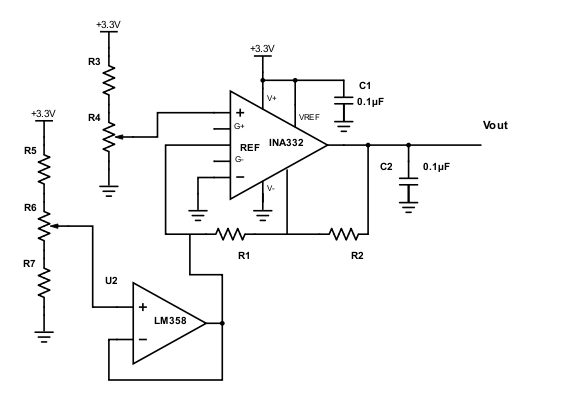
\includegraphics[width=\textwidth]{INA332-Test-Circuit}
	\caption{INA332 Test Circuit}
	\label{fig:INA332_Test_Circuit}
\end{figure}

\noindent The INA332 instrumentation amplifier is used to measure the force applied to a load cell. The amplification of this amplifier is given from the datasheet as Equation \ref{eqn:ina332-gain}. Since the load cell needed an amplification of at least 100, the calculated resistances were $R_1$ = 10k$\Omega$ and $R_2$ = 195k$\Omega$. The actual values selected for $R_1$ and $R_2$ were 10k$\Omega$ and 200k$\Omega$, respectively. This gives the amplifier an expected gain of ~105 V/V. See Figure \ref{fig:INA332_Test_Circuit} for the circuit diagram.

\begin{equation}
G = 5 + 5(\frac{R_1}{R_2})
\label{eqn:ina332-gain}
\end{equation}

\noindent The INA332 needs a voltage reference to use as the 0V differential output. Initially, two 1k$\Omega$ resistors were used to apply this voltage. This caused the output to change nonlinearly with the input voltage. The resistors were replaced with a LM358 dual operational amplifier, configured as a voltage buffer with the input connected to a potentiometer. The INA332 inputs were connected to ground and the LM358 buffer potentiometer was adjusted to set the 0V output to  $\frac{1}{2} V_{cc}$. This voltage was 1.846V. Instead of a potentiometer, two resistors were used to create this 1.846V offset.

\subsubsection{Hall Effect Encoder}
An Arduino Uno was used to ensure that the AS5055a absolute Hall effect encoder was functioning as we intended. Arduino makes rapid prototyping very easy by providing many libraries and a simple interface to quickly test a device without worrying about the board not functioning. Using the Arduino SPI library, the correct packets to send to the AS5055a were verified, along with the correct speed of both the SCLK and CS lines. The AS5055a datasheet specifies that the chip needs to receive a joint angle request at least every 0.6ms in order for the device to not go into low power mode. With this in mind, a sampling speed of 1kHz was selected.

\noindent In addition to the Arduino testing, tests were run with the TM4C123GH6PM and a test rig. %todo Add pictures of encoder test rig

\subsubsection{TM4C123GXL Launchpad}
Selecting a microcontroller was a key part of making the joint control board. Without a capable MCU, the joint board would not be able to function as we want it to, but buying the best microcontroller on the market can be costly. The EK-TM4C123GXL is an ARM Coretex M4f-based microcontroller evaluation kit from TI that has many peripherals to allow us to control the joint board without buying many external peripherals. The perihperals on this chip that we will need include a CAN controller, 12-bit ADC, USB controller, SSI controller, PWM controller, and many GPIO. These perihperals were implemented separately with a test circuit configured to verify that each peripheral was functioning correctly.

\noindent Several peripherals were needed to achieve the desired functionality from our microcontroller. A test board was set up in order to test and verify that each of these peripherals was setup properly and working as expected. The test board consisted of a potentiometer connected to an ADC pin, an SPI controlled ADC (MCP3202), the 1:2 demultiplexer (SN74LVC1G18), CAN transceiver (TC332), and some LEDs.

\noindent As a temporary stand in for the AS5055 absolute Hall effect encoder to test the SSI peripheral, a MCP3202 12-bit, 2 channel ADC was used. Both devices use SPI to communicate their sensor data back to the MCU, and the packets are similar in structure. Some differences between the two that can be changed are a maximum sample rate for the AS5055 of ~1ms as opposed to the few SCLK cycle delays for the MCP3202. The AS5055 has a maximum SCLK frequency of up to 10MHz at 3.3V while the MCP3202 has a limit of 900kHz at 3.3V. 

\noindent The potentiometer was connected to PE0 which was enabled at AIN3. The ADC was set to sample at 1kHz with hardware oversampling 16x enabled. A timer was configured to start an ADC conversion every millisecond, and a GPIO pin was set to 0 every time the ADC finished a conversion and set to 1 when the ADC conversion began. The time necessary to sample once at 16x hardware oversampling was around 5$\mu$s.


\begin{table}[H]
	\centering
	\caption{ADC Selection}

\begin{tabular}{|c|c|c|c|c|}
\hline
& Supply & Sampling & SCLK & \\
Part name & Voltage (V) & rate (MHz) & Freq (MHz) & Price (\$) \\
\hline
ADS7042 & 3.3 & 1 & 16 & 2.65 \\

ADS7043 & 3.3 & 1 & 16 & 2.65 \\

ADS7044 & 3.3 & 1 & 16 & 2.65 \\

ADC121S021 & 3.3, 5 & 0.2 & 4 & 2.85 \\

ADC121S051 & 3.3, 5 & 0.5 & 4 & 3.31 \\

ADC121S101 & 3.3, 5 & 1 & 4 & 3.39 \\

ADC7476 & 3.3, 5 & 1 & 20 & 3.41 \\

MCP3201 & 3.3, 5 & 0.1 & 1.6 & 2.31 \\

MAX11665 & 3.3 & 0.5 & 8 & 2.73 \\
\hline
\end{tabular}

\label{tbl:ADC Selection}
\end{table}

\noindent Note: The MCP3202 is functionally the same as the MCP3201, except it has a second input channel.


\subsubsection{Hall Effect Encoder}
An Arduino Uno was used to ensure that the AS5055a absolute Hall effect encoder was functioning as we intended. Arduino makes rapid prototyping very easy by providing many libraries and a simple interface to quickly test a device without worrying about the board not functioning. Using the Arduino SPI library, the correct packets to send to the AS5055a were verified, along with the correct speed of both the SCLK and CS lines. The AS5055a datasheet specifies that the chip needs to receive a joint angle request at least every
%TODO: Finish paragraph


%TODO: Make images smaller
\begin{figure}[H]
\centering
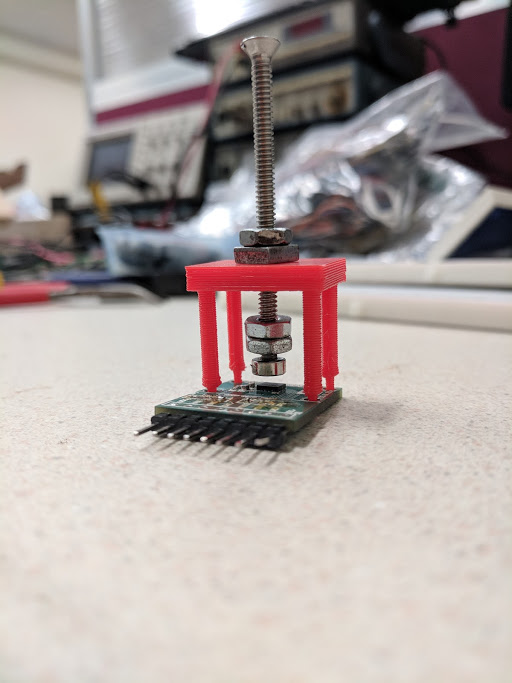
\includegraphics[width=\textwidth]{encoderTestRig1}
\caption{First Iteration of Encoder Test Rig}
\label{fig:First Iteration of Encoder Test Rig}
\end{figure}


\begin{figure}[H]
	\centering
	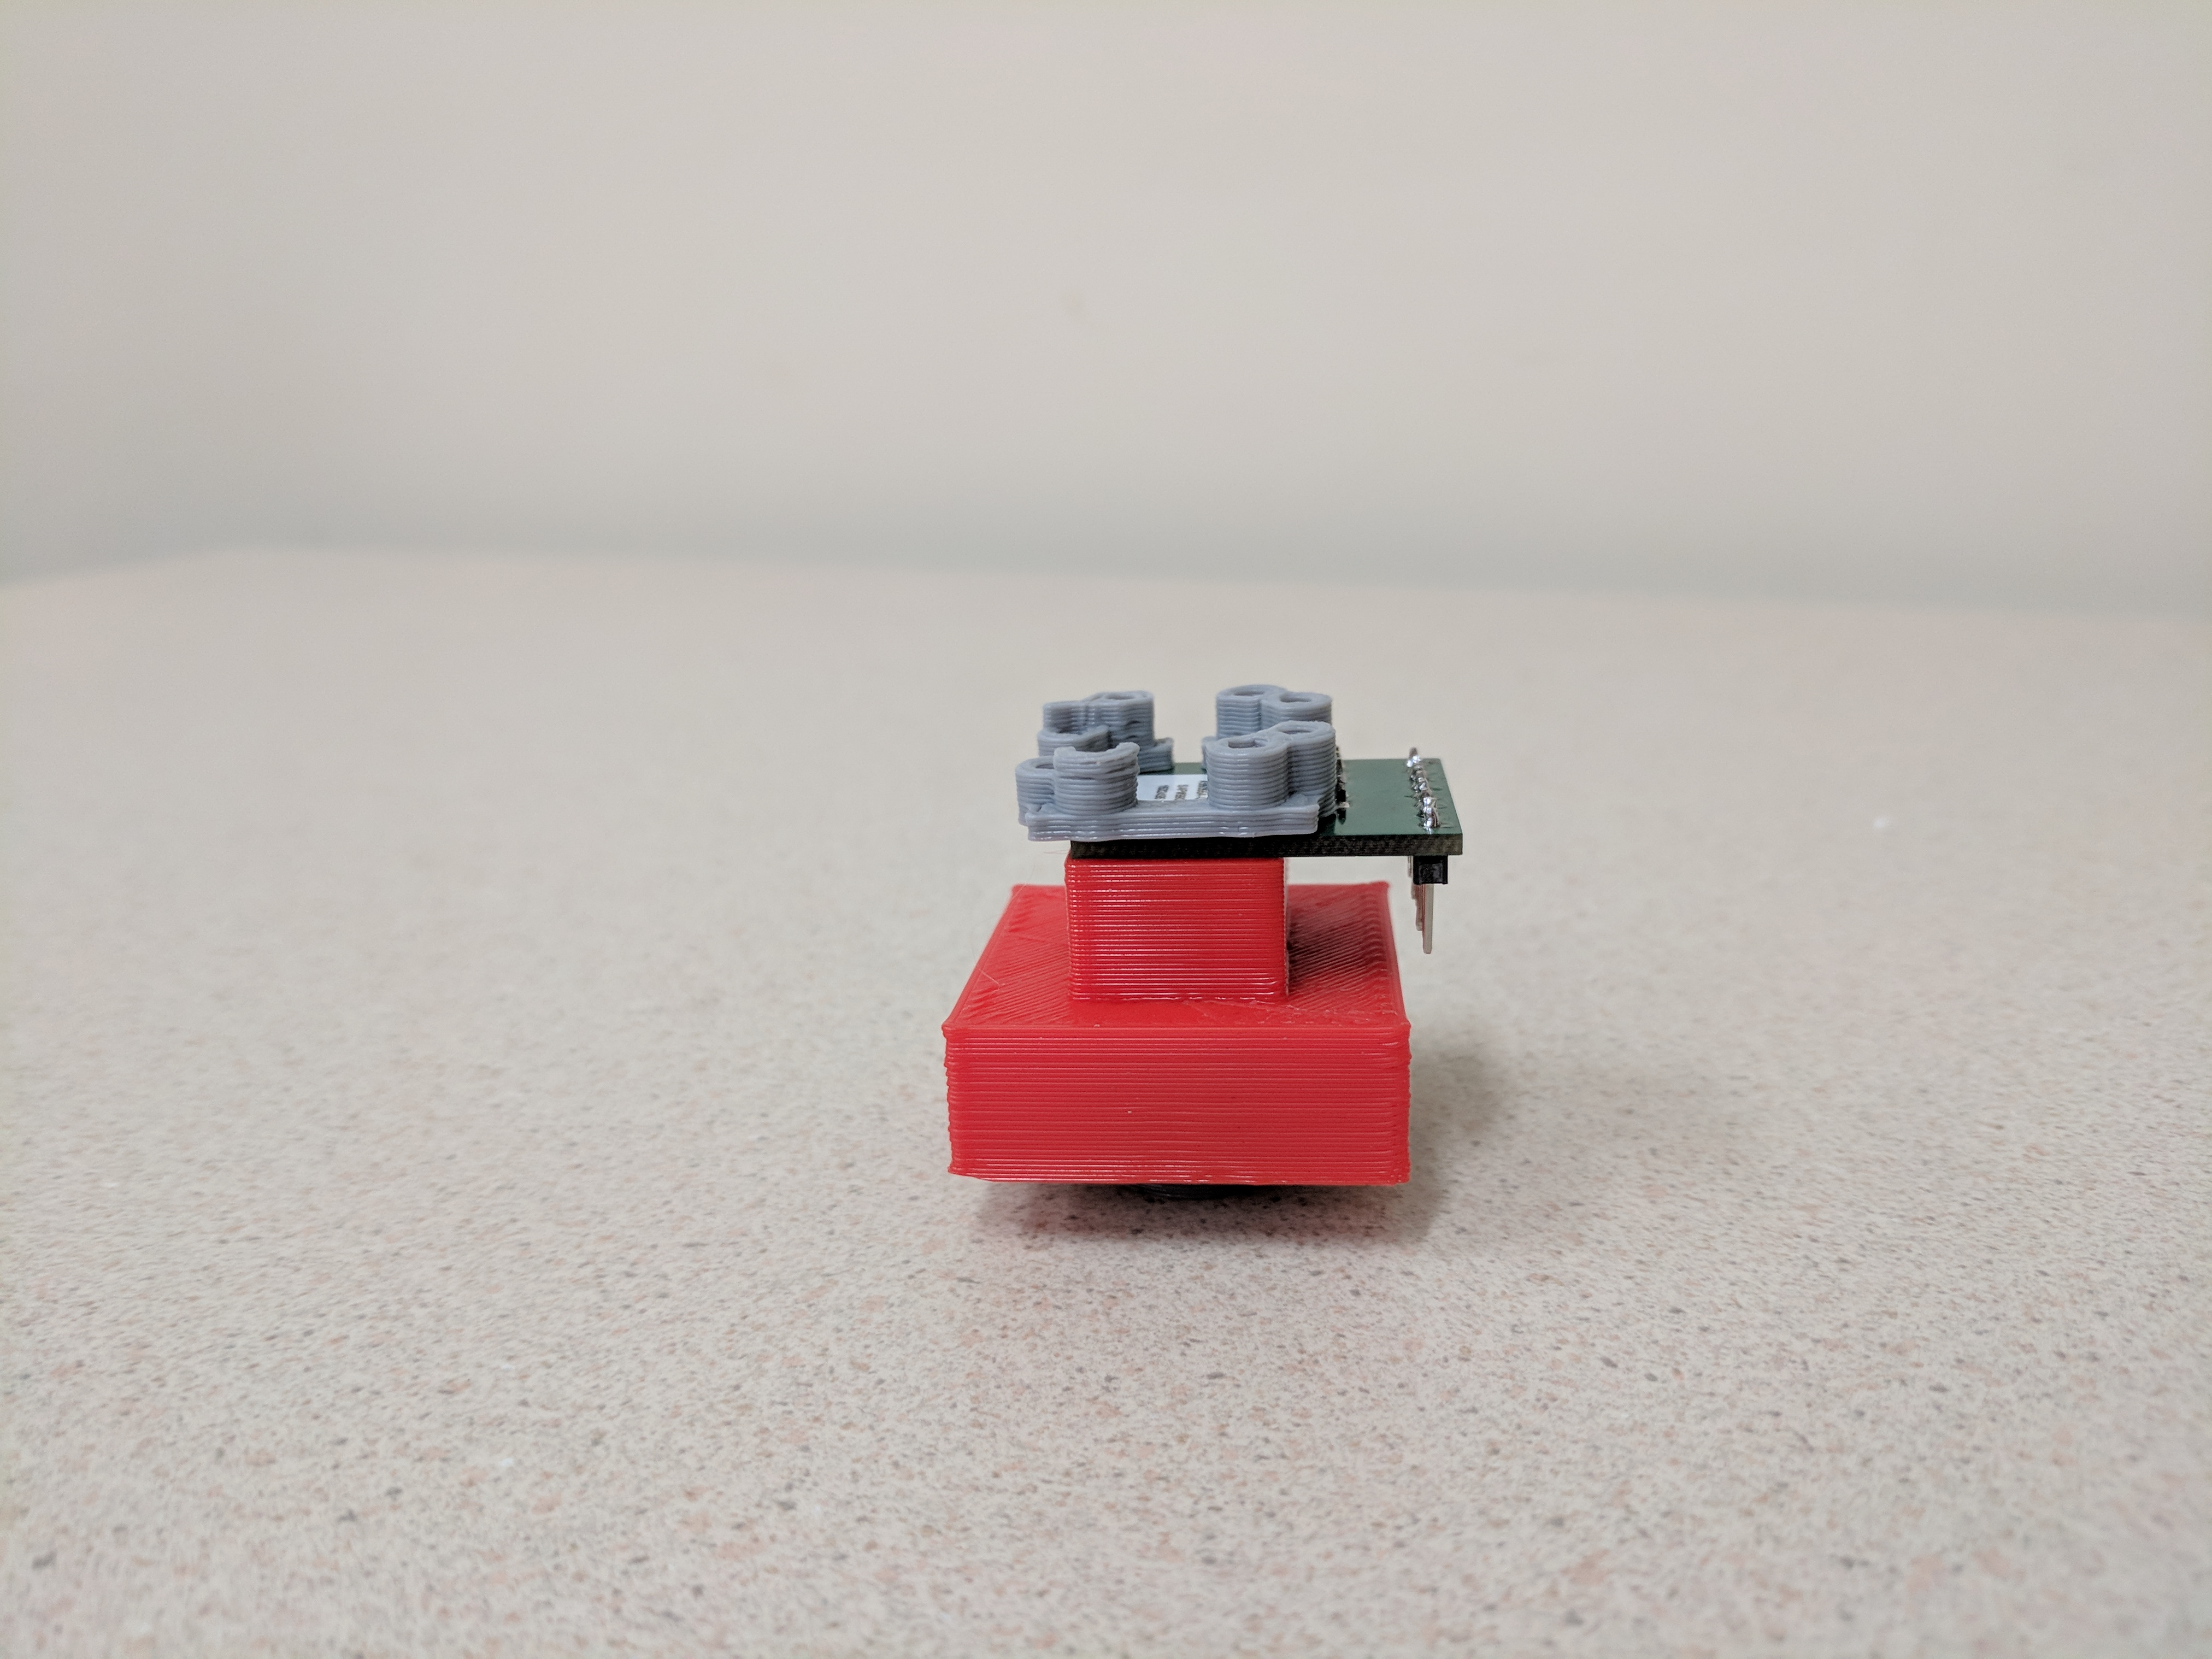
\includegraphics[width=\textwidth]{hallEffect2side}
	\caption{Second Iteration of Encoder Test Rig, Side View}
	\label{fig:Second Iteration of Encoder Test Rig, Side View}
\end{figure}

\begin{figure}[H]
	\centering
	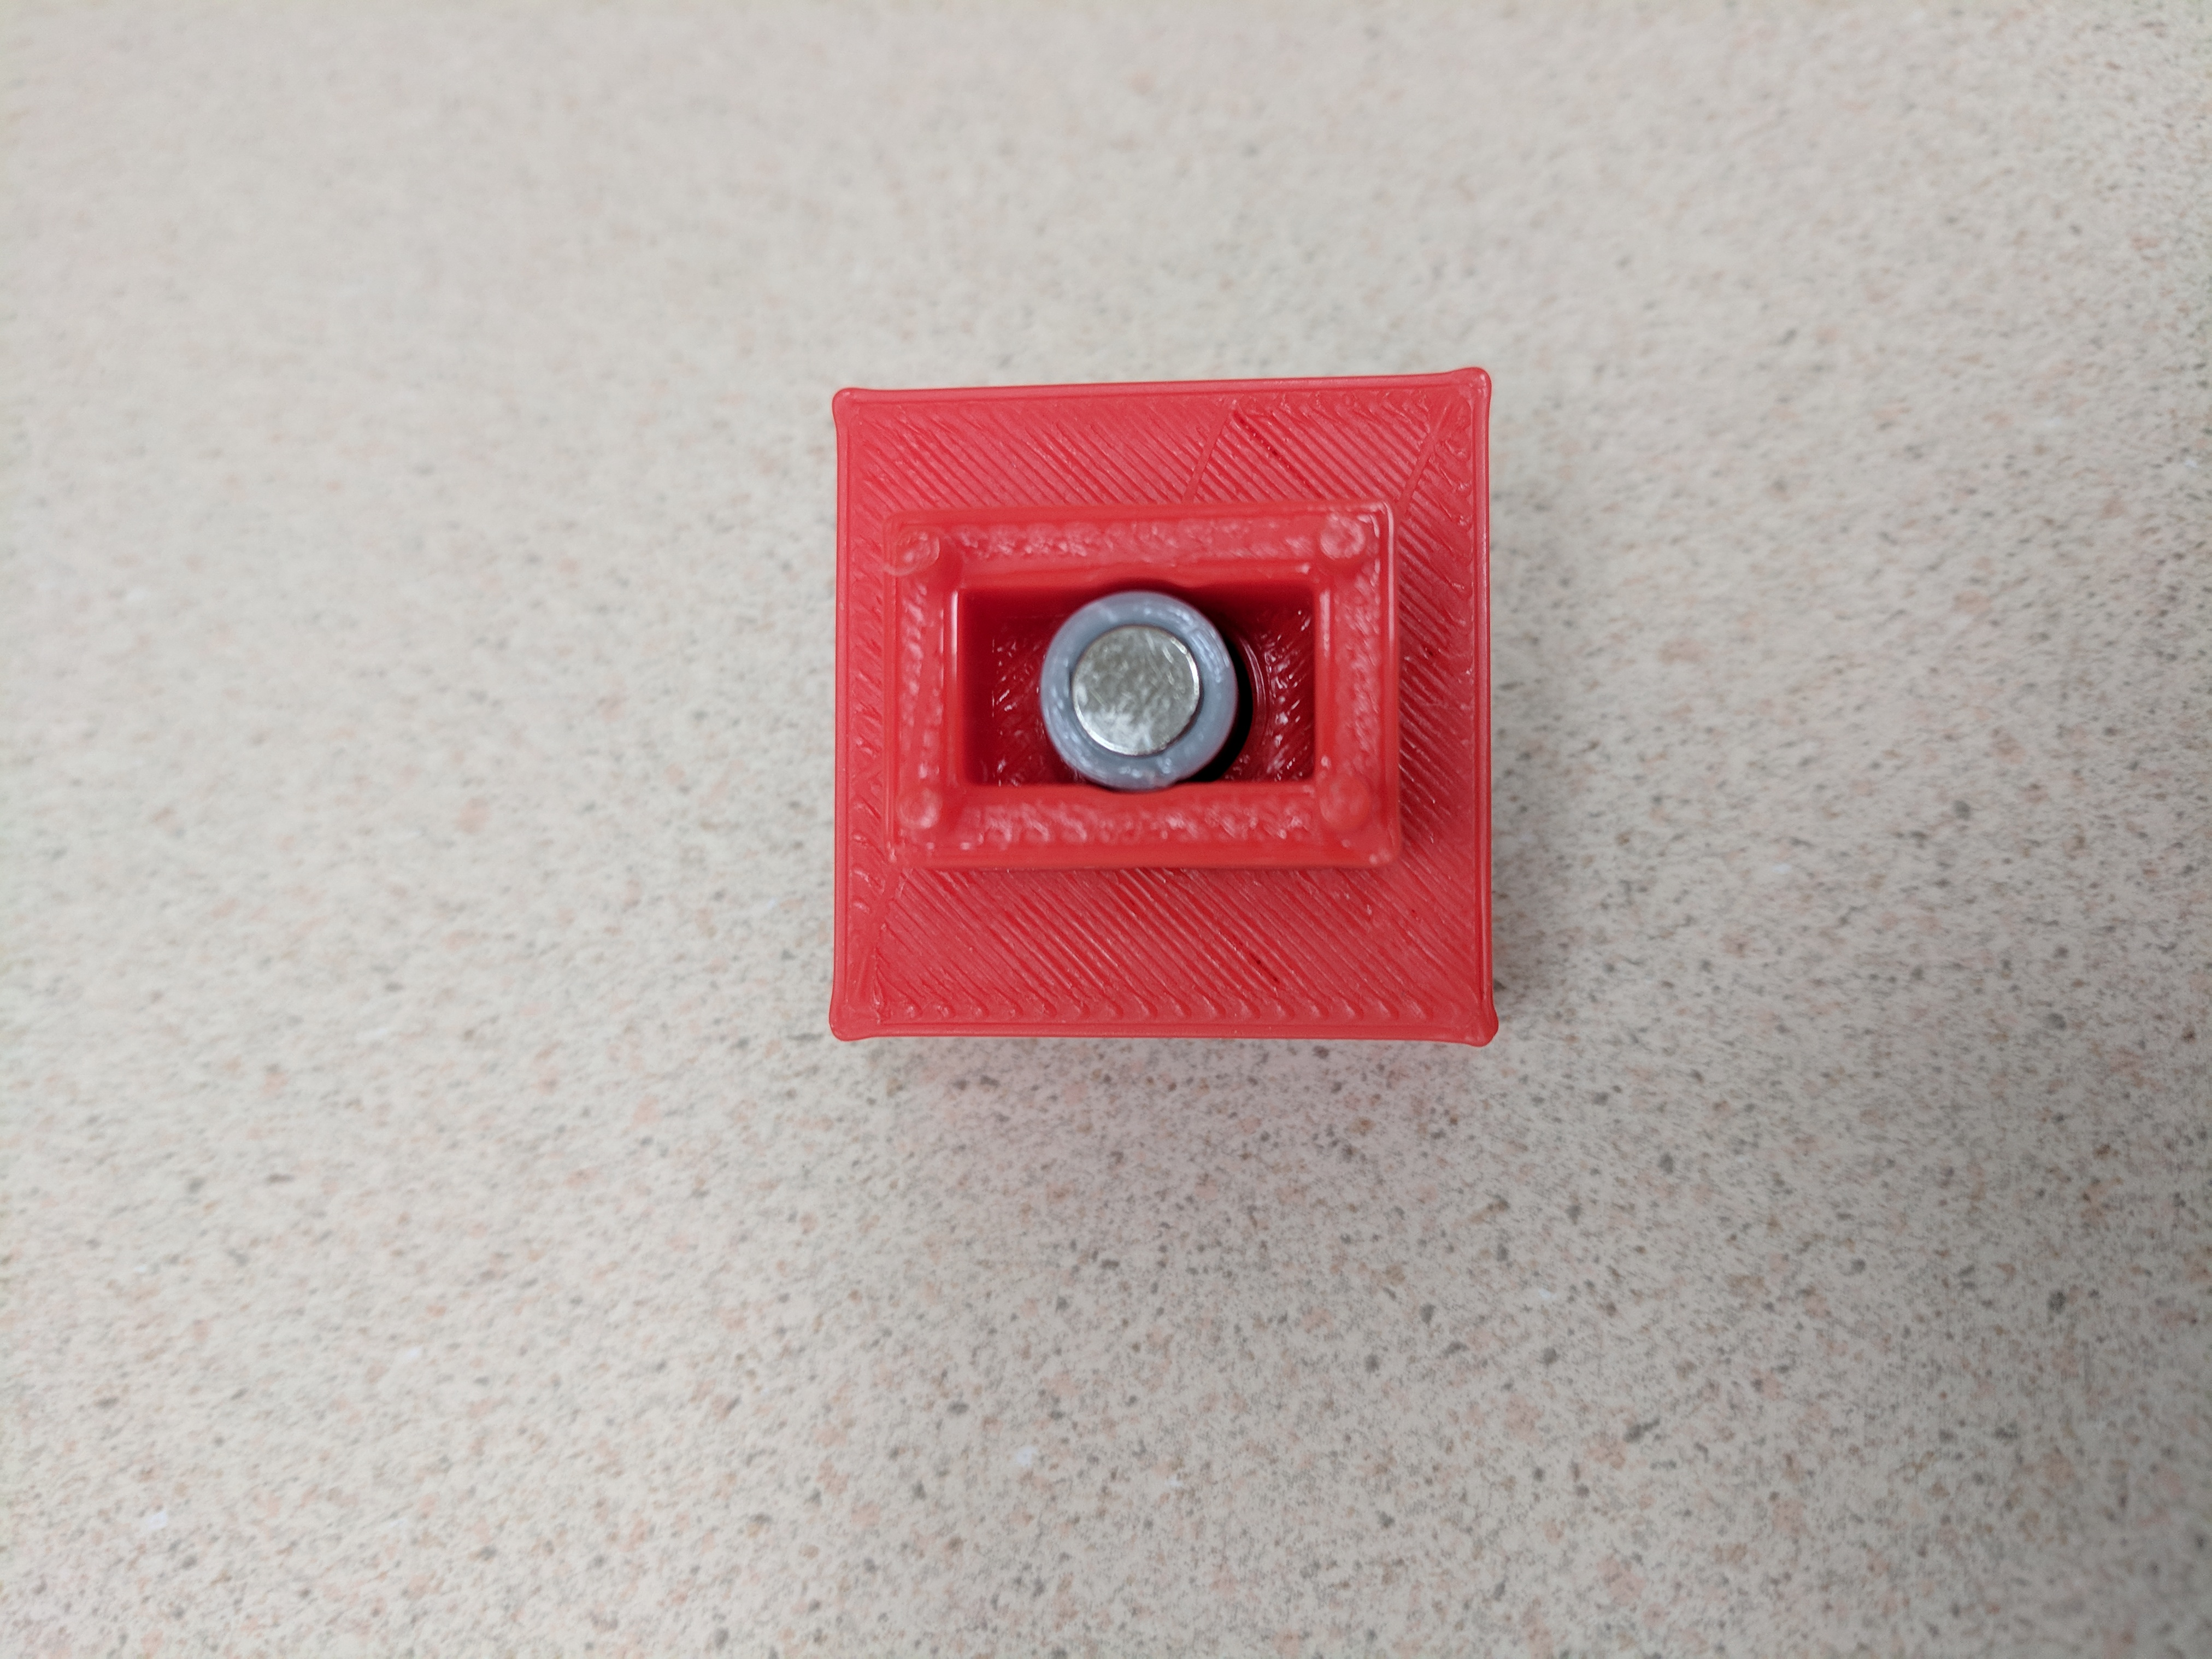
\includegraphics[width=\textwidth]{hallEffect2Top}
	\caption{Second Iteration of Encoder Test Rig, Magnet View}
	\label{fig:Second Iteration of Encoder Test Rig, Magnet View}
\end{figure}

\subsection{CAN Bus}
The CAN bus is the spine of the control system, carrying messages from the base to each joint and back from each of the joints to the base. Unit tests and careful integration were done to 

\subsubsection{Determining Joint Placement with Message ID}
CAN bus will be used to communicate between the base and joints. A limitation of CAN is that there is no way of determining the position of a module on the bus. This is important for controlling a robot arm since joint 1 is controlled differently from joint 2, etc. In order to determine the position of a joint board on the bus, another method is needed. The CAN message ID contains 11 bits in the standard frame.

\noindent We decided to use the upper 6 bits as a joint board number identifier, a number unique to that specific joint board, and the lower 5 bits as a message type. By doing this, we can tell the base the joint identifier number and position on the arm to rout position update messages to the correct joint on the arm.

\noindent There were a few ways of accomplishing this. One would be to program each joint board with a different identifier number. This could get very tedious and confusing for having many joint boards, since we would have to change and track identifier numbers for each unique joint board. Another option was to use EEPROM to automatically store the identifier number and upload it via the USB cable used for programming the board. This could get complicated since we would have to write code to not only read in the identifier properly, but also store it in EEPROM properly. Instead, we decided to use DIP switches. DIP switches allow us to input the identifier number in binary and update them on the fly without reprogramming the board.

\begin{figure}[H]
\centering
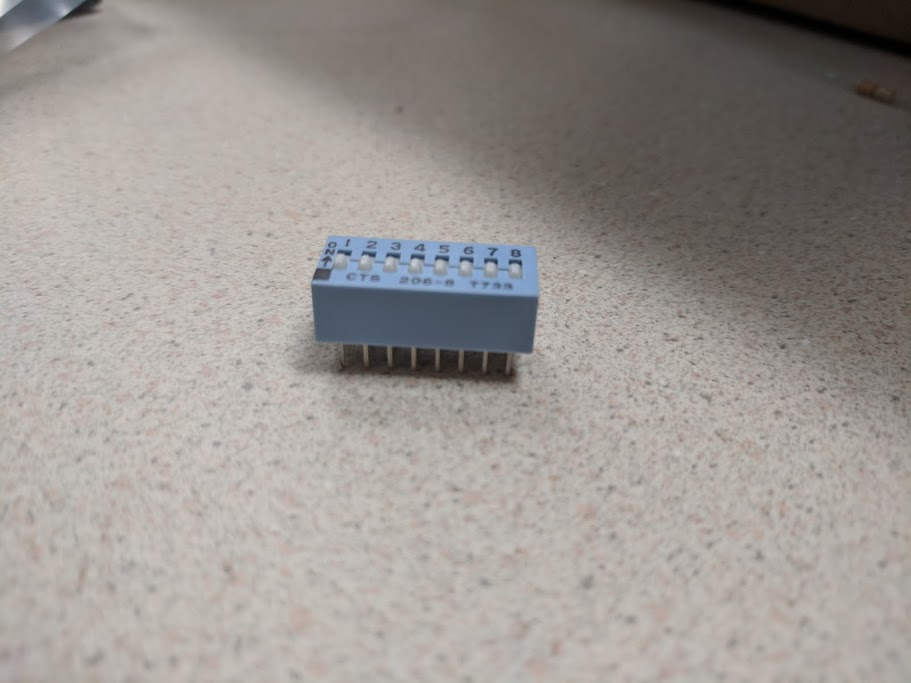
\includegraphics[scale=0.2]{cuteDipSwitch}
\caption{8-channel DIP Switch}
\label{fig:8_channel DIP Switch}
\end{figure}

\noindent On startup, the joint board reads in the identifier bits and stores them in a variable. The identifier is then used as a mask for the CAN message receive IDs. The CAN controller compares incoming message IDs to the ID mask and ID value set when initializing the message receive object. When setting the message receive object, we can set the message ID to the joint board identifier, shifted up by 5 bits, and set the mask to only listen for messages that match the upper 6 bits. We can set the message receive object to receive messages with the joint board ID in the upper 6 bits, regardless of message type. Since there are 32 message objects available on the CAN controller of the TM4C123GH6PM microcontroller, we have a great amount of flexibility for listening to different types of messages.

\begin{table}
	\centering
	\caption{CAN message ID breakdown}
	\begin{tabular}{| c | c |}
		\hline
		CAN ID & Message type \\
		\hline
		\textsc{000000XXXXX} & Reserved \\
		\textsc{XXXXXX00000} & Init Encoder \\
		\textsc{XXXXXX00001} & Init PID P constant \\
		\textsc{XXXXXX00010} & Init PID I constant \\
		\textsc{XXXXXX00011} & Init PID D constant \\
		\textsc{XXXXXX00100} & Position update to joint \\
		\textsc{XXXXXX10000} & Position update to base\\
		\hline
	\end{tabular}
\end{table}

\subsubsection{Implementing a Simple CAN Bus}
The preliminary CAN setup consisted of two TM4C Launchpads, one with transmit code and one with receive code. The transmitting board was set up for 1Mbps transmission with message ID = 2, and message length = 1 byte. The message data was a 4-bit value that incremented every time the message was successfully transmitted. A software delay was used to slow the transmission rate down to about every ~second. The receive board was set up for 1Mbps transmission with message ID = 0, message ID mask = 0, and message length = 1 byte. Setting both the message ID and mask to 0 signals the controller to accept any message. 4 LEDs were set up to see the CAN message data visually.
%TODO: insert table of configuration data

\noindent We had several problems getting this simple example to work. Initially, one of the jumper wires used for the CAN bus was broken, causing the CAN Hi lines on the transceivers to not be connected. The next problem was that the sample code provided by TI was not correct. When the CAN controller receives a valid message, it signals the processor with an interrupt. When a receive interrupt is processed by the example code, the interrupt flag is cleared and then the message data is read in. The problem is that when the interrupt flag is cleared, the new data bit that signals that there is valid data available is cleared. To fix this, the operations must be switched so that message data is read in before the interrupt flag is cleared. Once this fix was applied, CAN communications were functional. 

\noindent During the debugging process, a logic analyzer (Saleae 8-channel logic analyzer) was used to verify correct transmission of CAN packets. The logic analyzer software can be seen in Figure \ref{fig:can_logic_analyzer} decoding a packet with ID 2, data length 1, data byte equaling 7, and a proper ACK signal. The x marks a bit that was inserted to keep the timing consistent among the transceivers. Additionally, Figure \ref{fig:can_TXD_RXD} shows the ACK bit on the RXD line (channel 2) and no ACK bit on the TXD line (channel 0).

\begin{figure}[H]
	\centering
	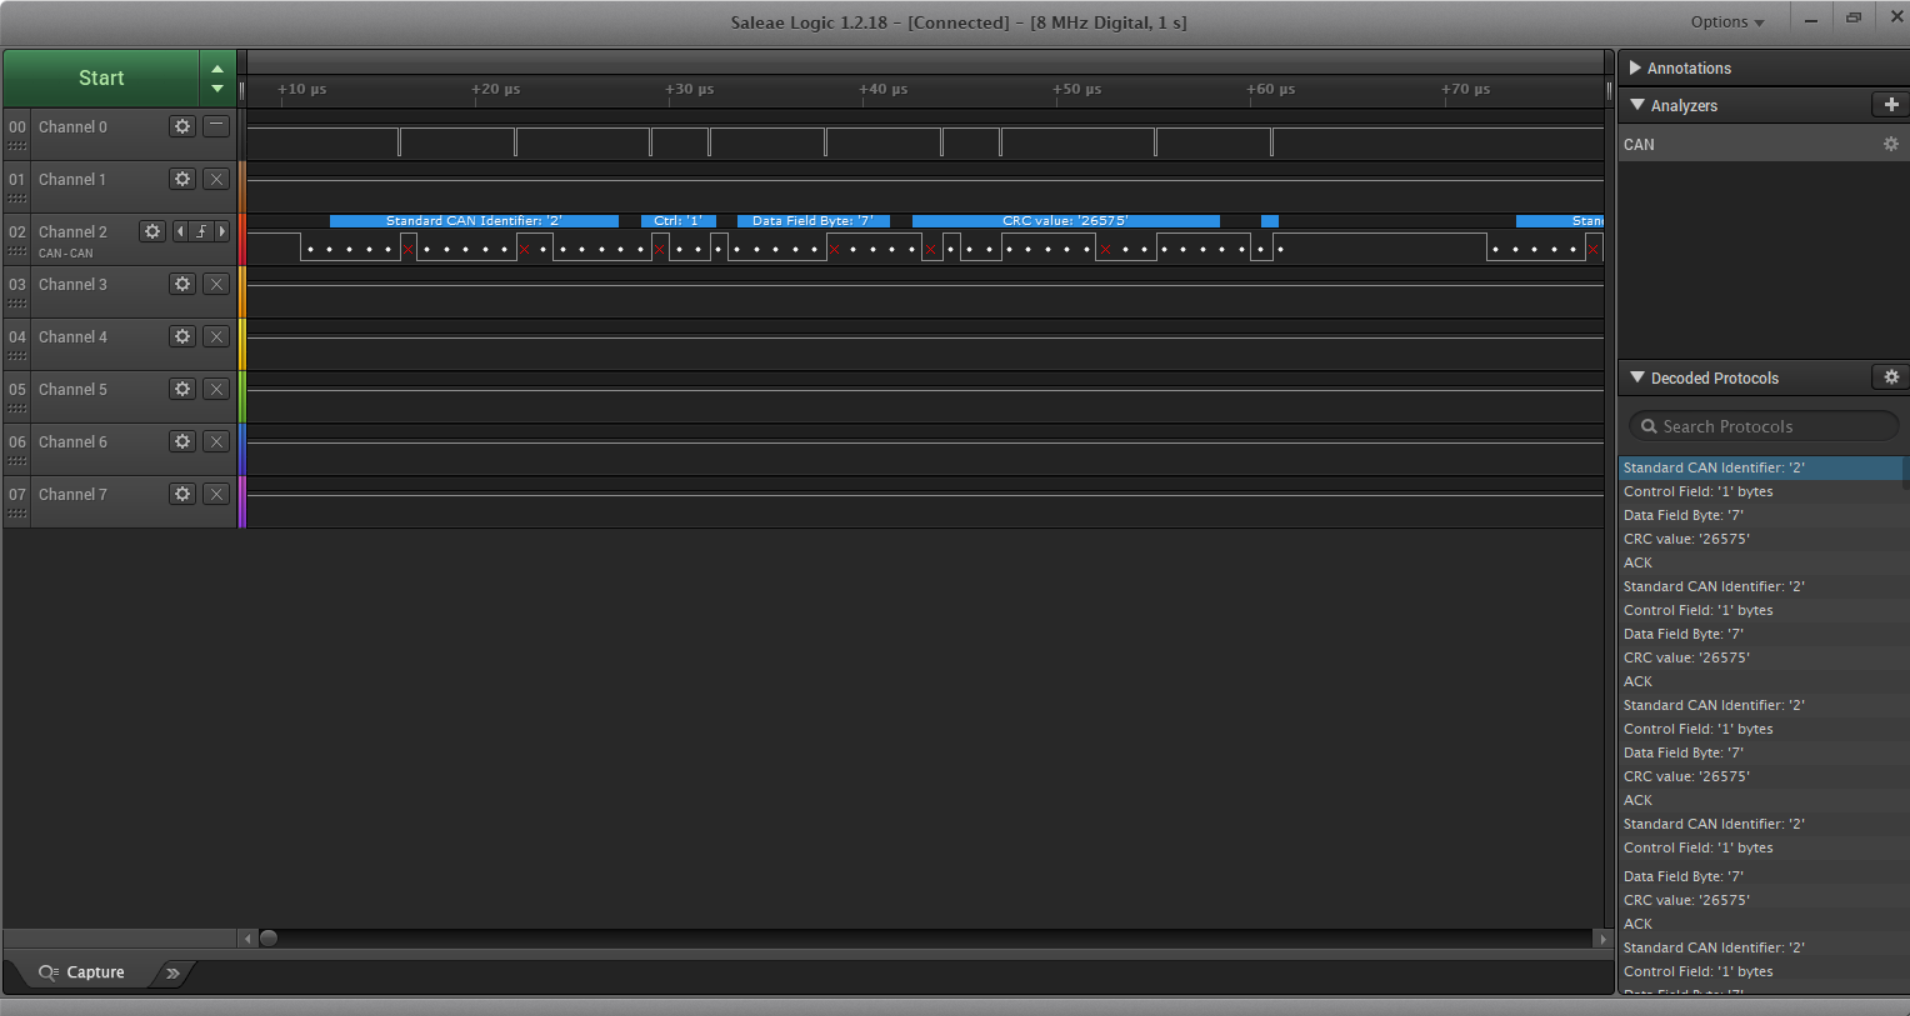
\includegraphics[width=\textwidth]{CAN_Logic_Analyzer}
	\caption{CAN bus as viewed in the logic analyzer software}
	\label{fig:can_logic_analyzer}
\end{figure}

\begin{figure}[H]
	\centering
	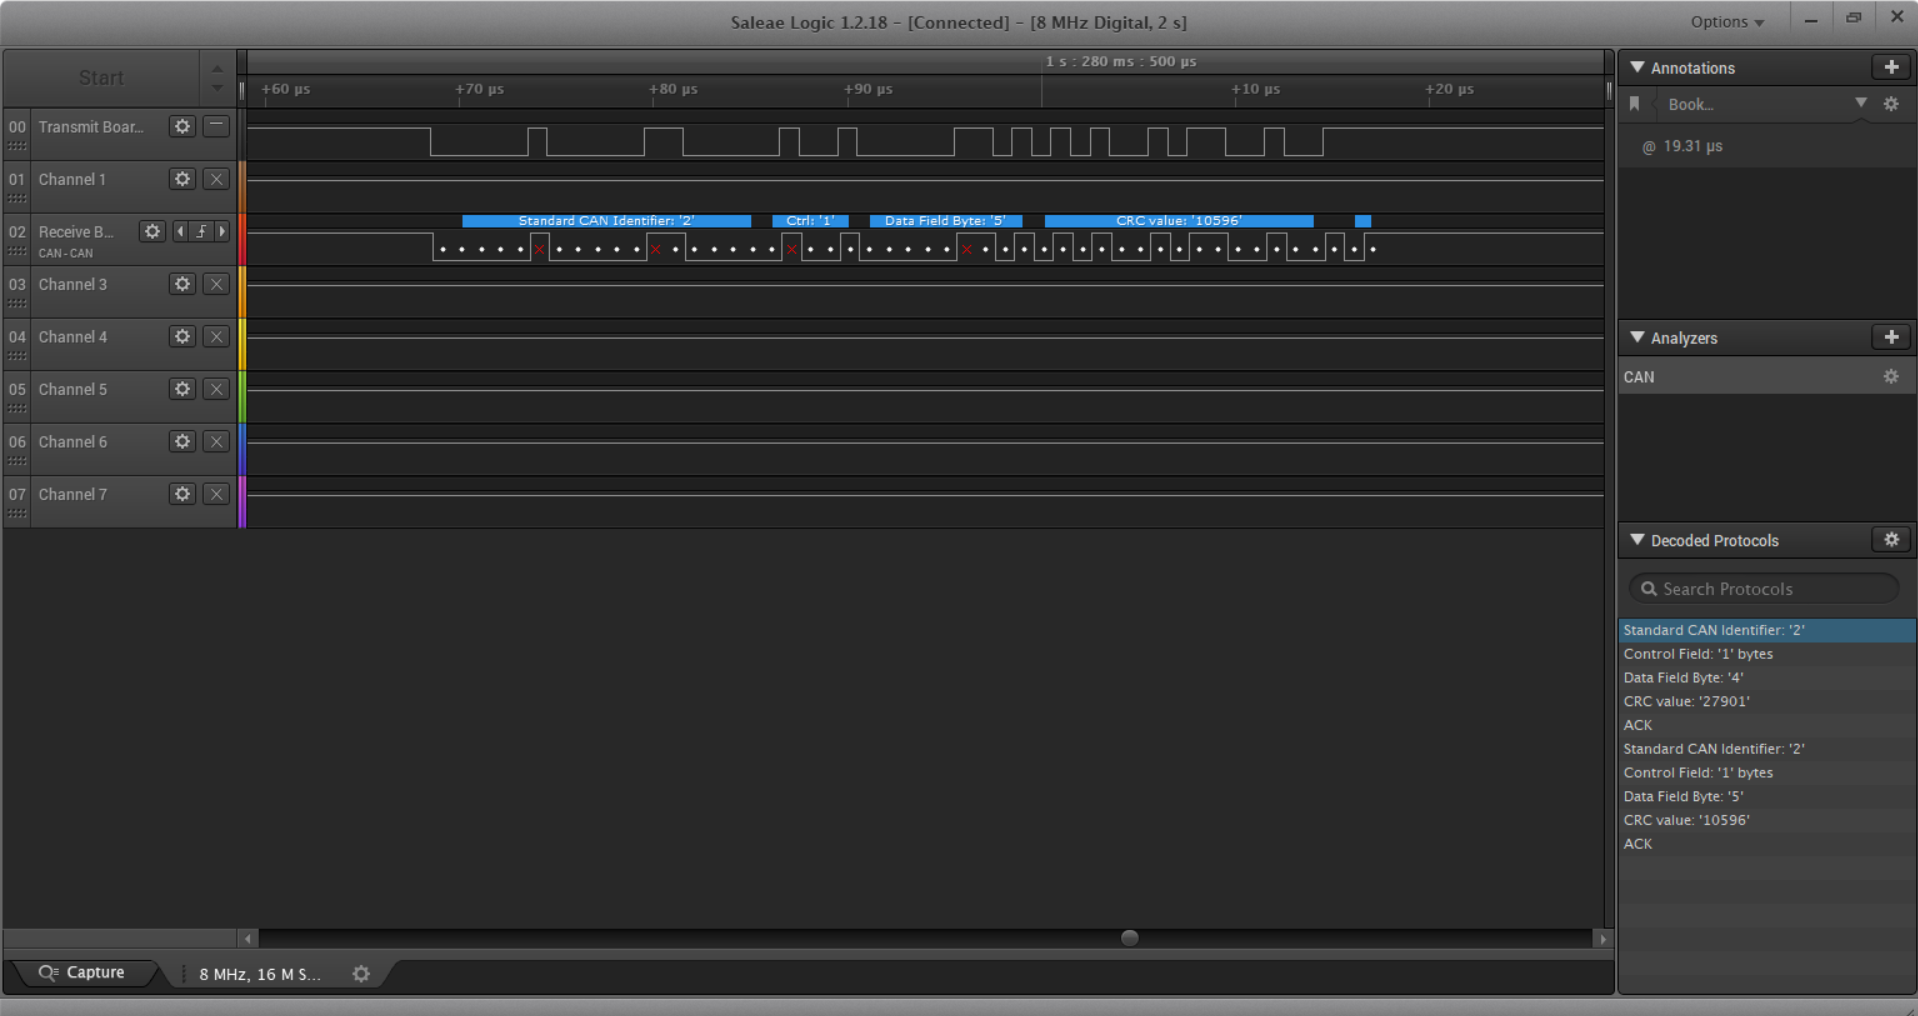
\includegraphics[width=\textwidth]{CAN_TXD_to_RXD}
	\caption{CAN TXD (channel 0) and RXD (channel 2) in the logic analyzer software}
	\label{fig:can_TXD_RXD}
\end{figure}

\subsubsection{CAN Termination}
CAN specification states that the CAN bus needs to be terminated on both ends by 120$\Omega$ resistors. The purpose of these resistors is to help mitigate signal reflections as well as pull the CAN Hi and CAN Lo lines together when the bus state is recessive. Since the resistors need to be at either end of the CAN bus, using normal resistors requires a static bus configuration. Out system will not necessarily have a fixed configuration, though, so a different solution was needed.

\noindent One method was to require the end user to attach a unique component, such as an end effector, at either end of the bus. This would effectively mean that an arm would always need a base module and an end effector to function properly. This rigid definition was not something we wanted to enforce on the end user, so instead we came up with a auto-disconnect circuit to disconnect the terminating resistor if another joint is added to the arm.

\noindent The way this works is through a MOSFET switch, seen in Figure \ref{fig:can_terminate_circ}. The MOSFET (part number BS170) drain and source connect the CAN Hi and CAN Lo lines through a 120$\Omega$ resistor and the gate is pulled up to $V_{DD}$ through a 1l$\Omega$ resistor. When the next joint is connected, the gate is connected to ground and the MOSFET is opened, disconnecting the CAN Hi and CAN Lo lines. When there is no joint connected, the MOSFET is closed, effectively acting as a 5$\Omega$ resistor in series with the 120$\Omega$ resistor. This new 125$\Omega$ resistance is within tolerance in the CAN specifications which state that the resistance must be between 50$\Omega$ and 70$\Omega$.
%todo: cite BS170 datasheet

\begin{figure}[H]
	\centering
	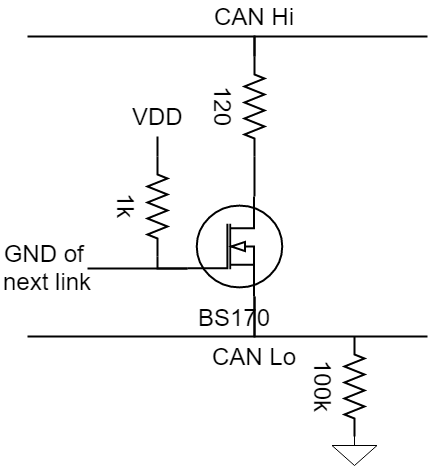
\includegraphics[scale=0.5]{CAN_terminate}
	\caption{CAN bus auto-terminate circuit}
	\label{fig:can_terminate_circ}
\end{figure}

\subsection{Printed Circuit Boards}
A PCB was made for each of the major subsystems as a more final test. The subsystems for which a PCB was designed include the motor driver (both with and without a current sensor), load cell amplifier, CAN transceiver, and TM4C123GH6PM microcontroller. After these were verified to be working, a Boosterpack compatible design of the whole joint control board.

\noindent The motor driver PCB can be seen in Appendix \ref{app:motor_driver} and has the demultiplexer and a shunt resistor for triggering the automatic internal shutoff if the current gets too high. The motor driver with current sensor has a current sensor integrated in the board and can be seen in Appendix \ref{app:motor_driver_current}. The load cell amplifier has the LM358 op amp as well as the INA332 instrumentation amplifier and can be seen in Appendix \ref{app:load_cell_amp}. The CAN transceiver PCB was designed that contains the 6 necessary DIP switches, CAN transceiver, and auto-terminate circuit and can be seen in Appendix \ref{app:can_transceiver}. The joint control board Boosterpack has all of these components in a single PCB that mounts on top of the TM4C123GXL Launchpad and can be seen in Appendix \ref{app:joint_board_boosterpack}. All of these PCBs can be seen in Figure \ref{fig:pcbs}. A closeup of the joint control board Boosterpack attached to a Launchpad can be seen in Figure \ref{fig:jcb_boosterpack}.

\begin{figure}[H]
	\centering
	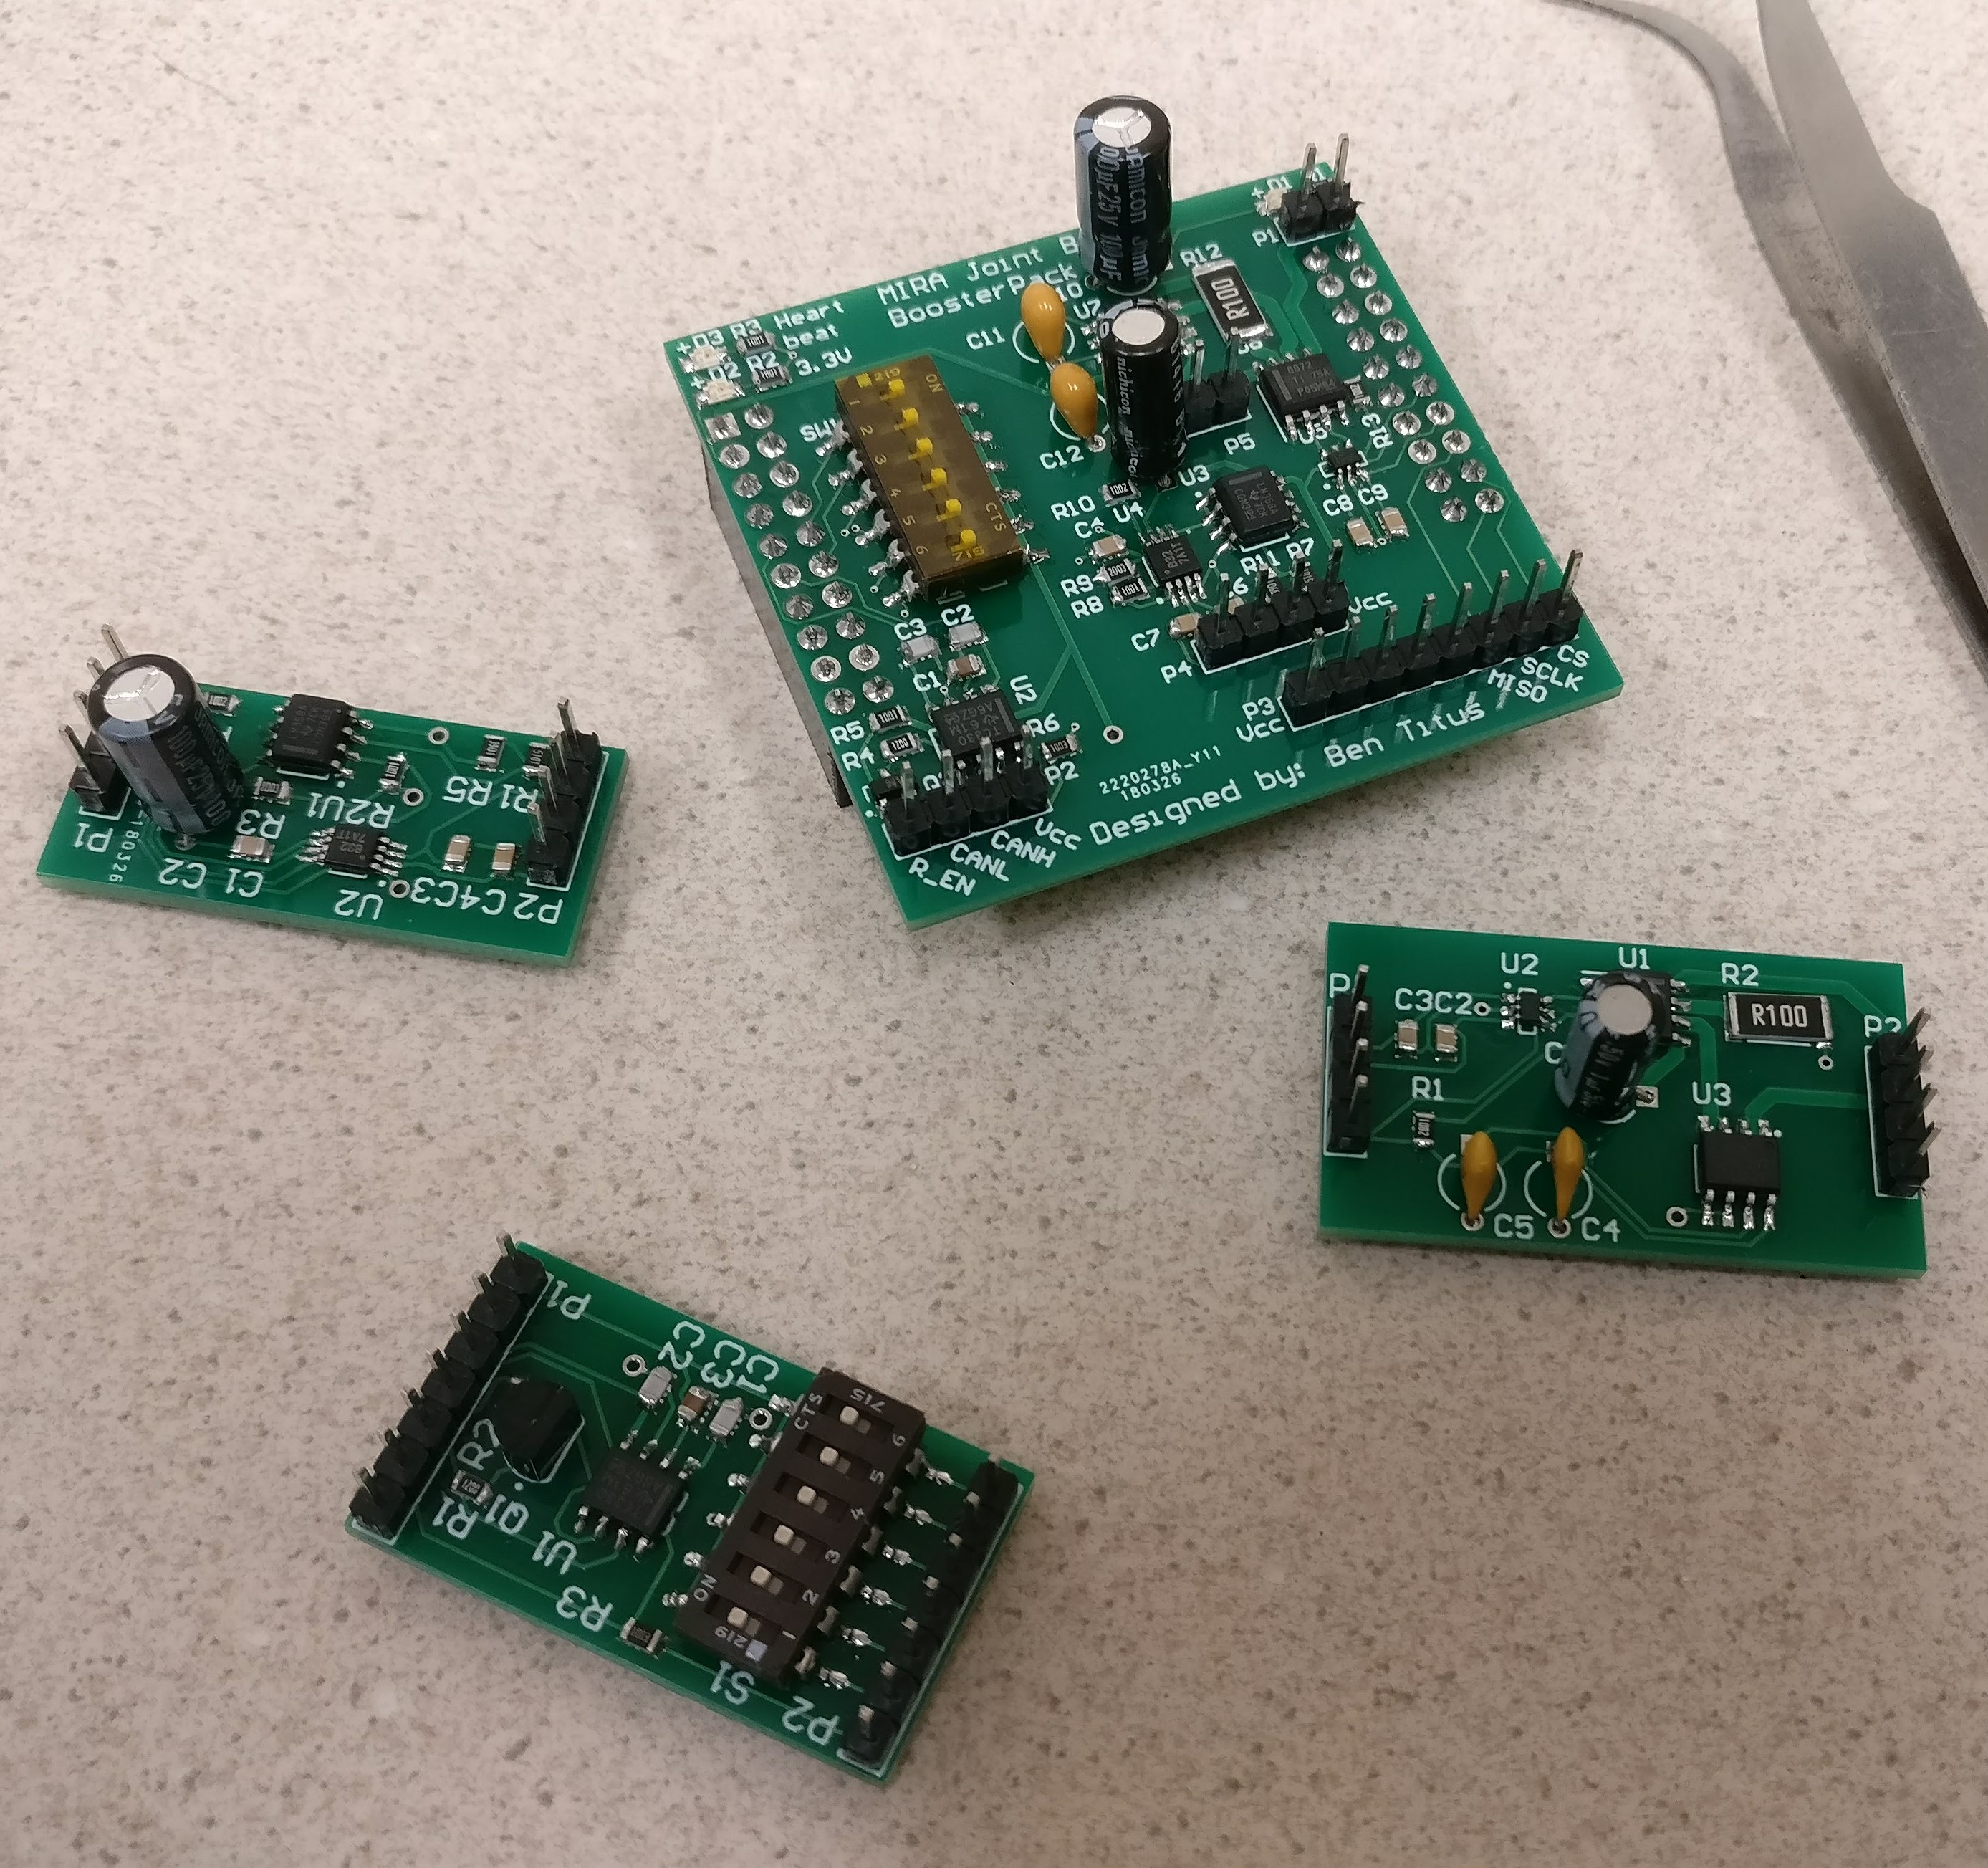
\includegraphics[scale=0.1]{pcbs}
	\caption{Assembled PCBs of each major subsystem including motor driver with current sensor (right), CAN transceiver (bottom), load cell amplifier (left), and joint control board Boosterpack (top)}
	\label{fig:pcbs}
\end{figure}

\begin{figure}[H]
\centering
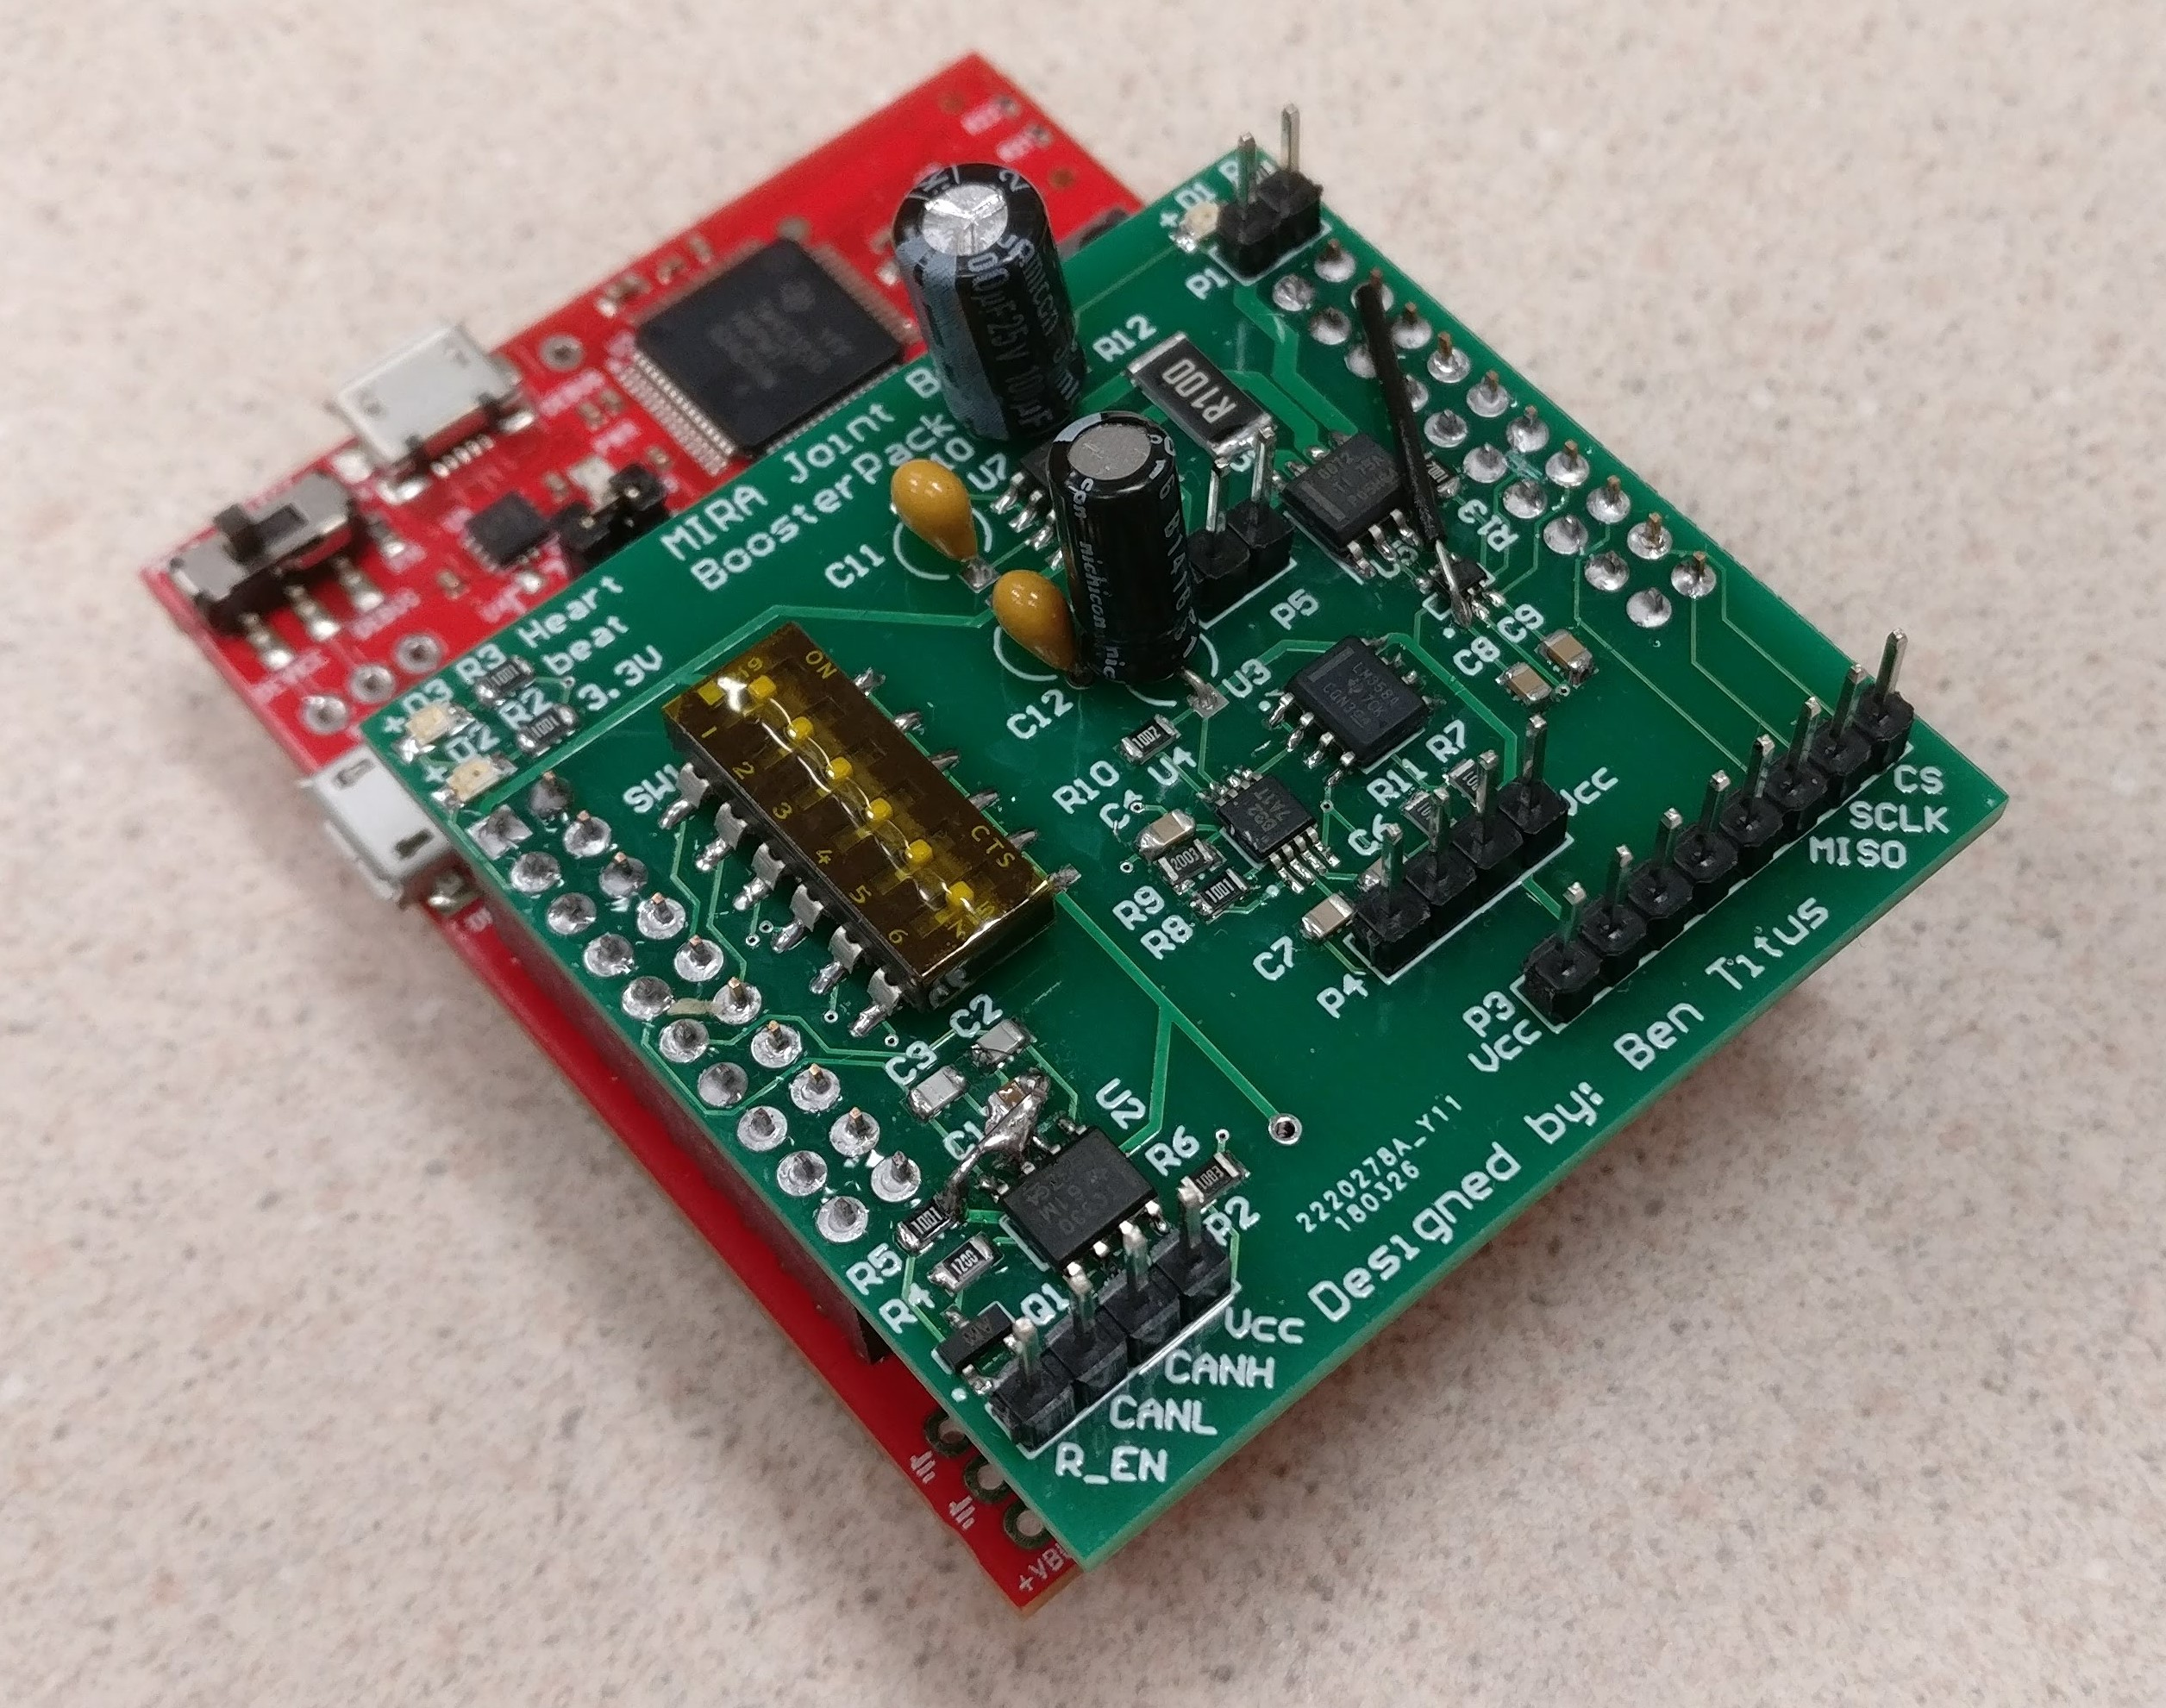
\includegraphics[scale=0.1]{jcb_boosterpack}
\caption{Joint control board Boosterpack on the TM4C123GXL Launchpad}
\label{fig:jcb_boosterpack}
\end{figure}

\noindent Small problems existed in some of the PCBs during the first revision. The CAN transceiver PCB has the $V_{CC}$ and GND pins swapped. Once this problem was identified, the traces were cut, wire soldered, and the schematic altered for another revision. The load cell amplifier PCB has a GND pin that was not connected to anything. The GND pin on the INA332 amplifier had an unconnected ground pin. This pin was connected with wire, and the PCB worked as expected.

\noindent The joint control board Boosterpack had the CAN transceiver $V_{CC}$ and GND pins swapped as well as needing the motor direction pin to be moved from one pin to another. This change came about due to the Launchpad construction. Two of the pins were connected internally but labeled differently, so the motor direction pin was swapped in code, the trace was cut, and wire was soldered to the new pin. These changes can be seen in Figure \ref{fig:jcb_boosterpack}. Another revision of the joint control board Boosterpack was made but not ordered due to time constraints.

\subsection{Arm Structure}
Arm structure is not something we wanted to fully define, since the end user is supposed to create their own arms, but there were some basic components that needed clarification. The first of these is that every arm must begin with a base module and have some combination of up to four additional joints connected.  This allows the end-user flexibility in how they want to construct the arm without allowing them to add too many joints.


\subsection{Code Library}
The code library is another important part of what we did to make our arm work. It controls all of the electrical components via the sending of packets out to the base module over a Serial UART line. It handle a lot of the more involved calculations for controlling the arm like the forward and inverse kinematics.  


\subsubsection{Maven}
Maven is a utility for Java-based projects that seeks to provide a uniform build system for the project. It accomplishes this by defining a project object model and a set of plugins that each Maven project shares. Therefore, Maven can provide a streamlined build environment for every instance of the project, allowing users to have the same build process across multiple different devices and environments. Maven could be compared to a flexible template for how a project should be arranged and what files should be included. We chose Maven for our Java project because it makes it much easier for our team to collaborate on the front-end side of the code.  It also allows us to package into our program libraries that we used in our project so that there are fewer dependencies that the end-user must download in order to use our software \cite{maven}.


\subsubsection{Program flow}
%TODO: Add link to explain what a class and object are

\begin{figure}[H]
\centering
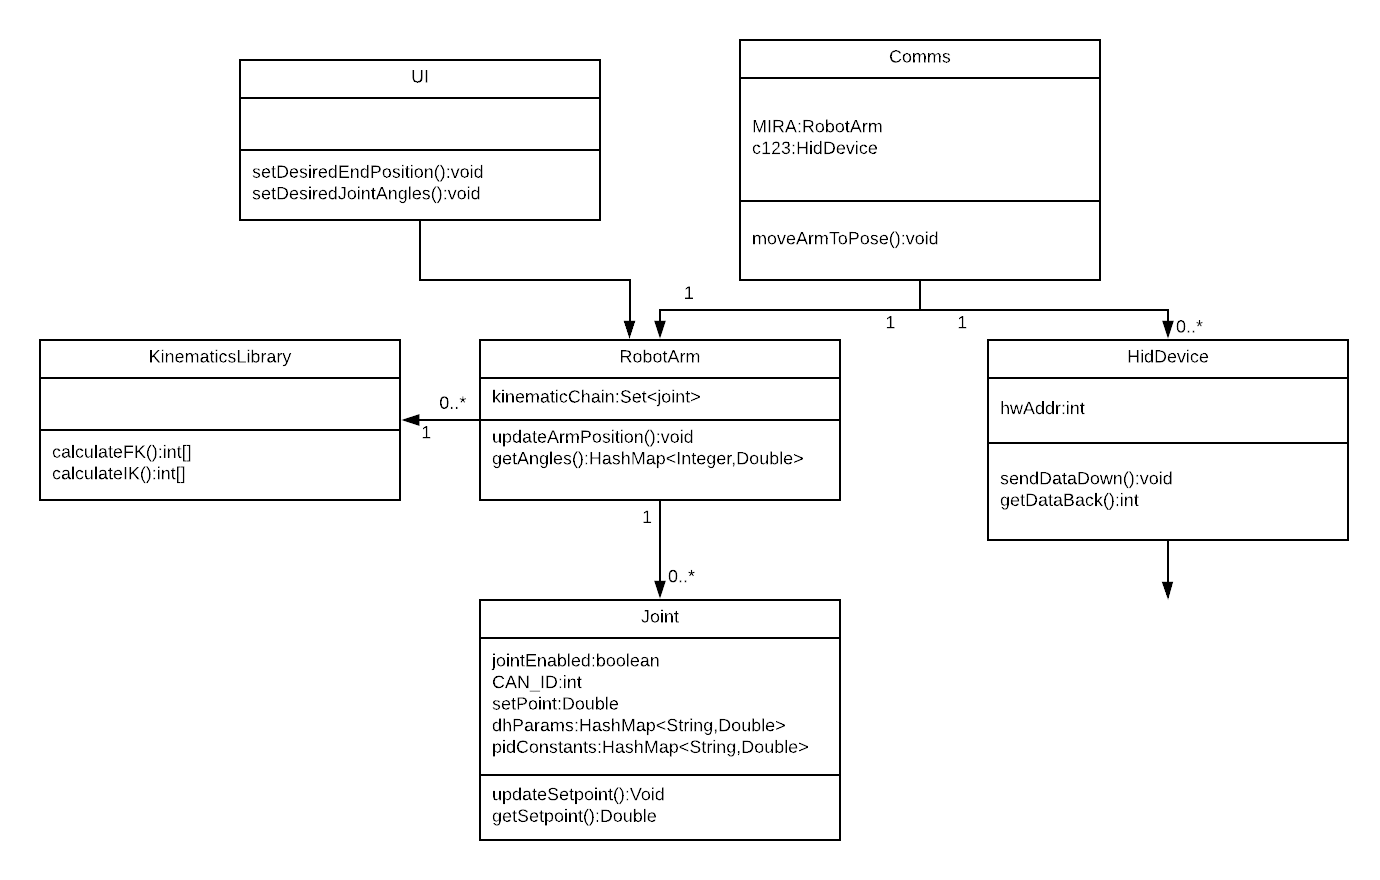
\includegraphics[width=\textwidth]{pc_Mira_UML}
\caption{UML Diagram showing different classes and their relations}
\label{fig:Functional_Block_Diagram}
\end{figure}

%TODO do something more with this sentence
\noindent The front-end program running on the PC is written in Java. We used JavaFX to make the GUI. We chose to write this part of the program in Java because of the speed and reliability of a language that has many libraries and excellent Interactive Development Environments.  

\noindent The main class starts the JavaFX Project. The JavaFX Project holds an list of joints which lists all the joints, which contains data about how the arm is configured. Each Joint object makes sure to tell the Comms object that it's time to send a message to the actual joint whenever new information about itself comes in. When the user enters new information about the arm into the GUI, the GUI's controller tells the joint object to change that information about itself. For example, if the user changes the setpoint of Joint 2 from 90 degrees to 112 degrees, the GUI will tell Joint 2 that its position has been updated to 112. Joint 2 will, upon seeing that its position has been updated, ask the Comms object to convey the new position information to the arm's base board.

\noindent The Joint object does not contain a Comms object inside itself. Rather, there is a single Comms object for the entire program to use. The Comms object follows the Singleton design pattern. A singleton is a class which can only ever be instantiated one time. Singletons are often used to hold configuration information about a program because they guarantee that if one object makes changes to the singleton's settings then any other object that subsequently asks for those settings will get back the most up-to-date version.

\noindent In this case, it makes sense to use a singleton because we want to guarantee that there's only a single place in the code which tries to access the serial port at any given time. Another way to accomplish this same goal would have been to move all of Comms's functions to inside the JavaFX controller. There is only one controller object. Arranging the program this way would have violated Java's design principles and would have made writing the code a battle rather than an art form. %Please don't take this out they're definitely not going to get this far into the paper anyway probably

\noindent Each joint would need to hold a reference to the JavaFX controller inside itself. Referencing such an architecture-specific piece of the program within the core of the program's logic would be bad for future portability of the code. 

\subsubsection{Serial Communication}
Serial communication is a very common protocol used to transmit data between a maximum of two devices over two lines, Rx and Tx. Serial communication is already available on our microcontroller through its universal asynchronous receiver/transmitter (UART). This device translates the Tx and Rx line into a parallel data bus that can interface with our microcontroller autonomously. The Java code interfaces directly with this UART over a USB line connected to both the Tiva board and the computer. The Java code holds a class called Comms which opens a specified serial port upon instantiation. This is implemented through the use of NRJavaSerial \cite{NRJavaSerial}, a library created by Kevin Harrington and used for serial communications over USB. Upon instantiation of the Comms singleton, we open the specified serial port on the computer and begin polling it at a baud rate of 115200. The enables the port to send and receive data so that the computer can send and receive messages from our base board. The Java code hold a buffer which acts as a First in First Out (FIFO) queue that is constantly updated when new data is received so that we can read in data that is on the serial line \cite{SerialSparkfun}.
Since we are only able to send individual bits at a time across the serial line, we need to encode and decode the data that we send.  We have to encode the data from ASCII strings into their decimal equivalents before sending them out over the serial line. Then upon receipt of data we must decode the data before it is able to be built into a string which represents one packet. Once we have individual packets available to us as strings, we can easily use Java's string comprehension functionality to update the necessary parts of the code and properly encode data for sending\cite{SerialSparkfun}.

\subsubsection{Mutltithreading}
Multithreading is the process of creating new threads in order to let code run in parallel. Creating a new thread in Java involves instantiating a new thread object from Java's standard libraries and passing in the relevant information to the Thread through the constructor \cite{ThreadJava}. The reason that we needed to use a thread is the need for a mode where the computer communicates over Serial, writing out and reading in data that it receives at a constant rate. The problem with this style of coding is that it requires a while loop which continuously executes code that would normally block all other pieces of code from running. Since we need to concurrently run our GUI and modify the values that we are sending to the arm based on GUI inputs, we cannot have the processor locked up all the time sending and receiving serial communications. Therefore, we created a new thread where serial communications could be handled on an entirely separate process than the GUI. We create this thread after the initialization of our arm has been completed and start it running when the arm has acknowledged that it is ready to begin communications. Therefore, without interfering with our GUI process, we are able to uphold constant serial communications without causing our GUI to crash mid-operation. Doing this allows us to move the joint sliders pictured below and have them constantly send out new messages to the arm telling the selected joint to turn to the new position. 

\begin{figure}[H]
	\centering
	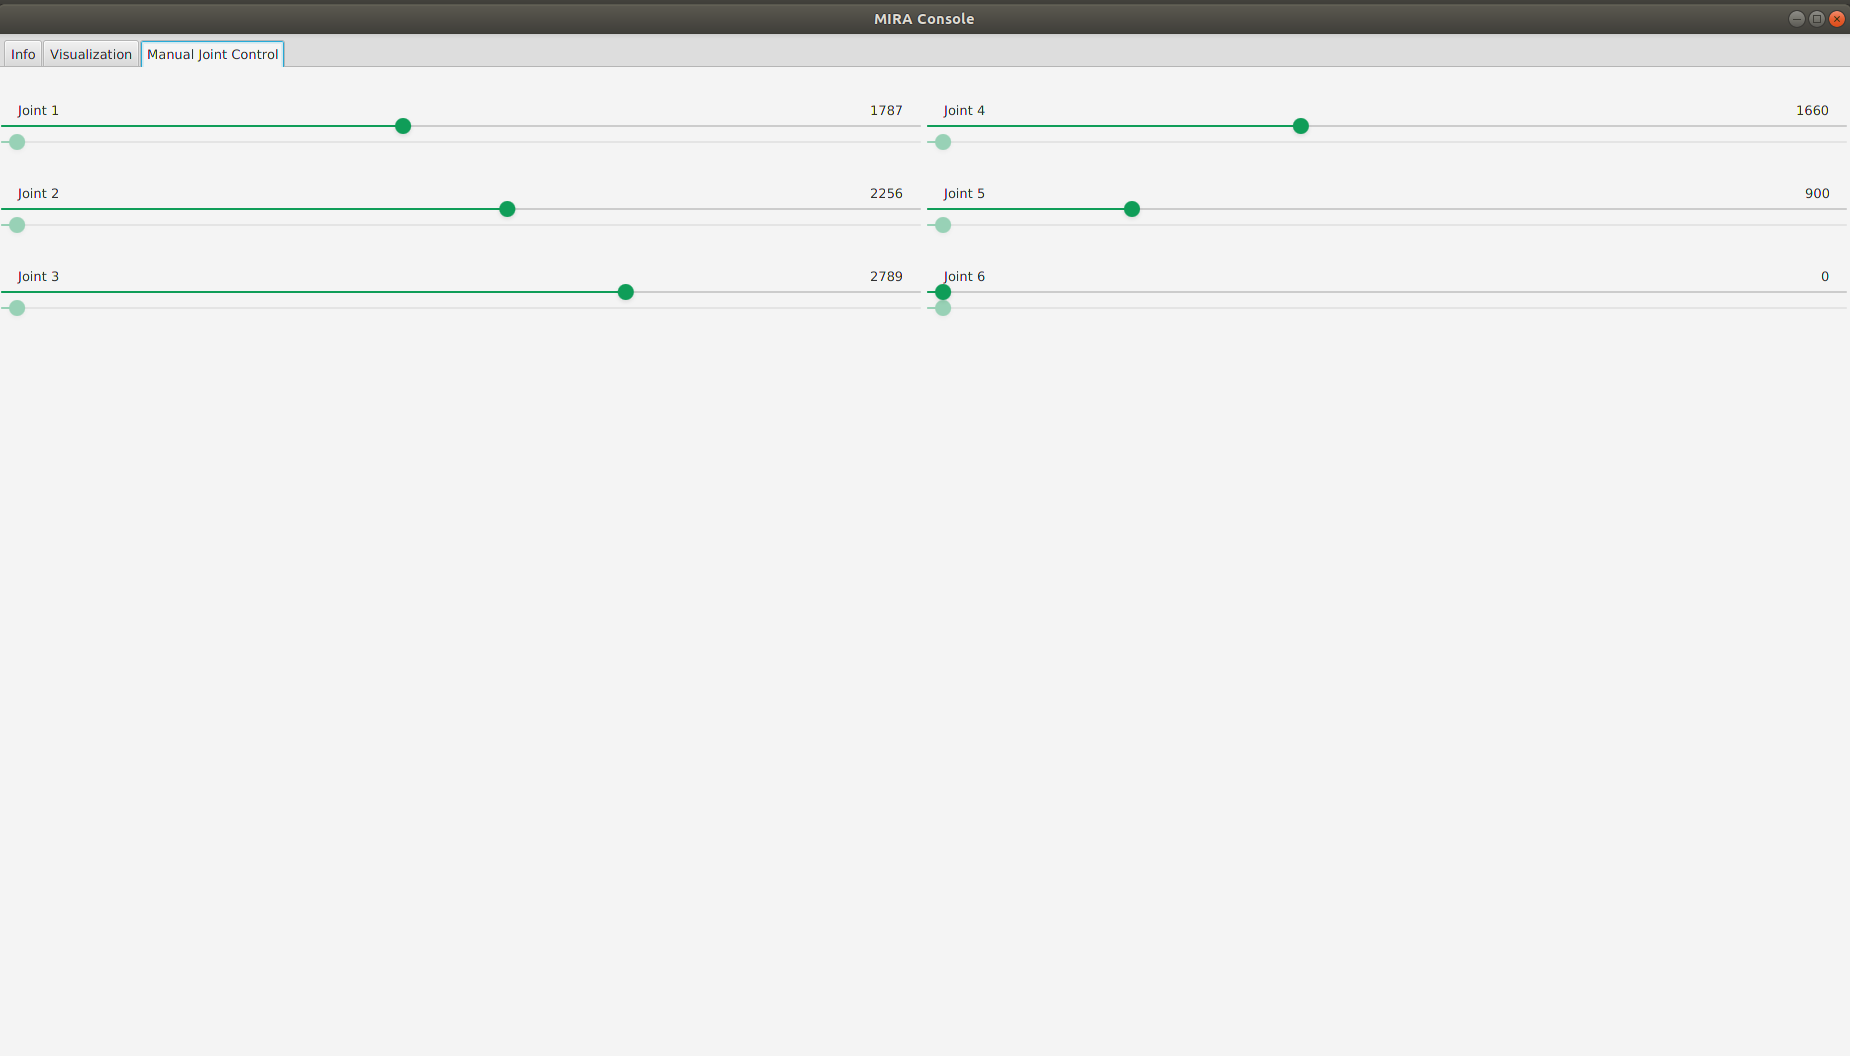
\includegraphics[width=\textwidth]{GUI_sliders}
	\caption{Image of the GUI tab which adjusts the setpoint for joints}
	\label{fig:GUI_Sliders}
\end{figure}


\subsubsection{Saving of Configuration}
%TODO: Talk about Gson
In order to store the information that we need to be persistent between different instances of the application, we used a library called Gson made by Google \cite{gson}. This library's primary use is to take data and store it in a .json file, a kind of simplistic database.  We used this library to save the joint object which were the data containers about the configuration of the arm. All of the saving and loading is done via the GUI so that the user can either load information about an arm themselves, or they can change the values using the GUI text fields and save a new configuration when it needs updating. Doing so allows the user to always be able to either modify and update the constants inside the data container that is the Joint object and have those objects be saved and loaded during each runtime of the application. Pictured below is the GUI tab which stores all of the constants for the arm such as encoder home values and PID constants, as well as has buttons to interface with the saving, loading and startup of our program.

\begin{figure}[H]
	\centering
	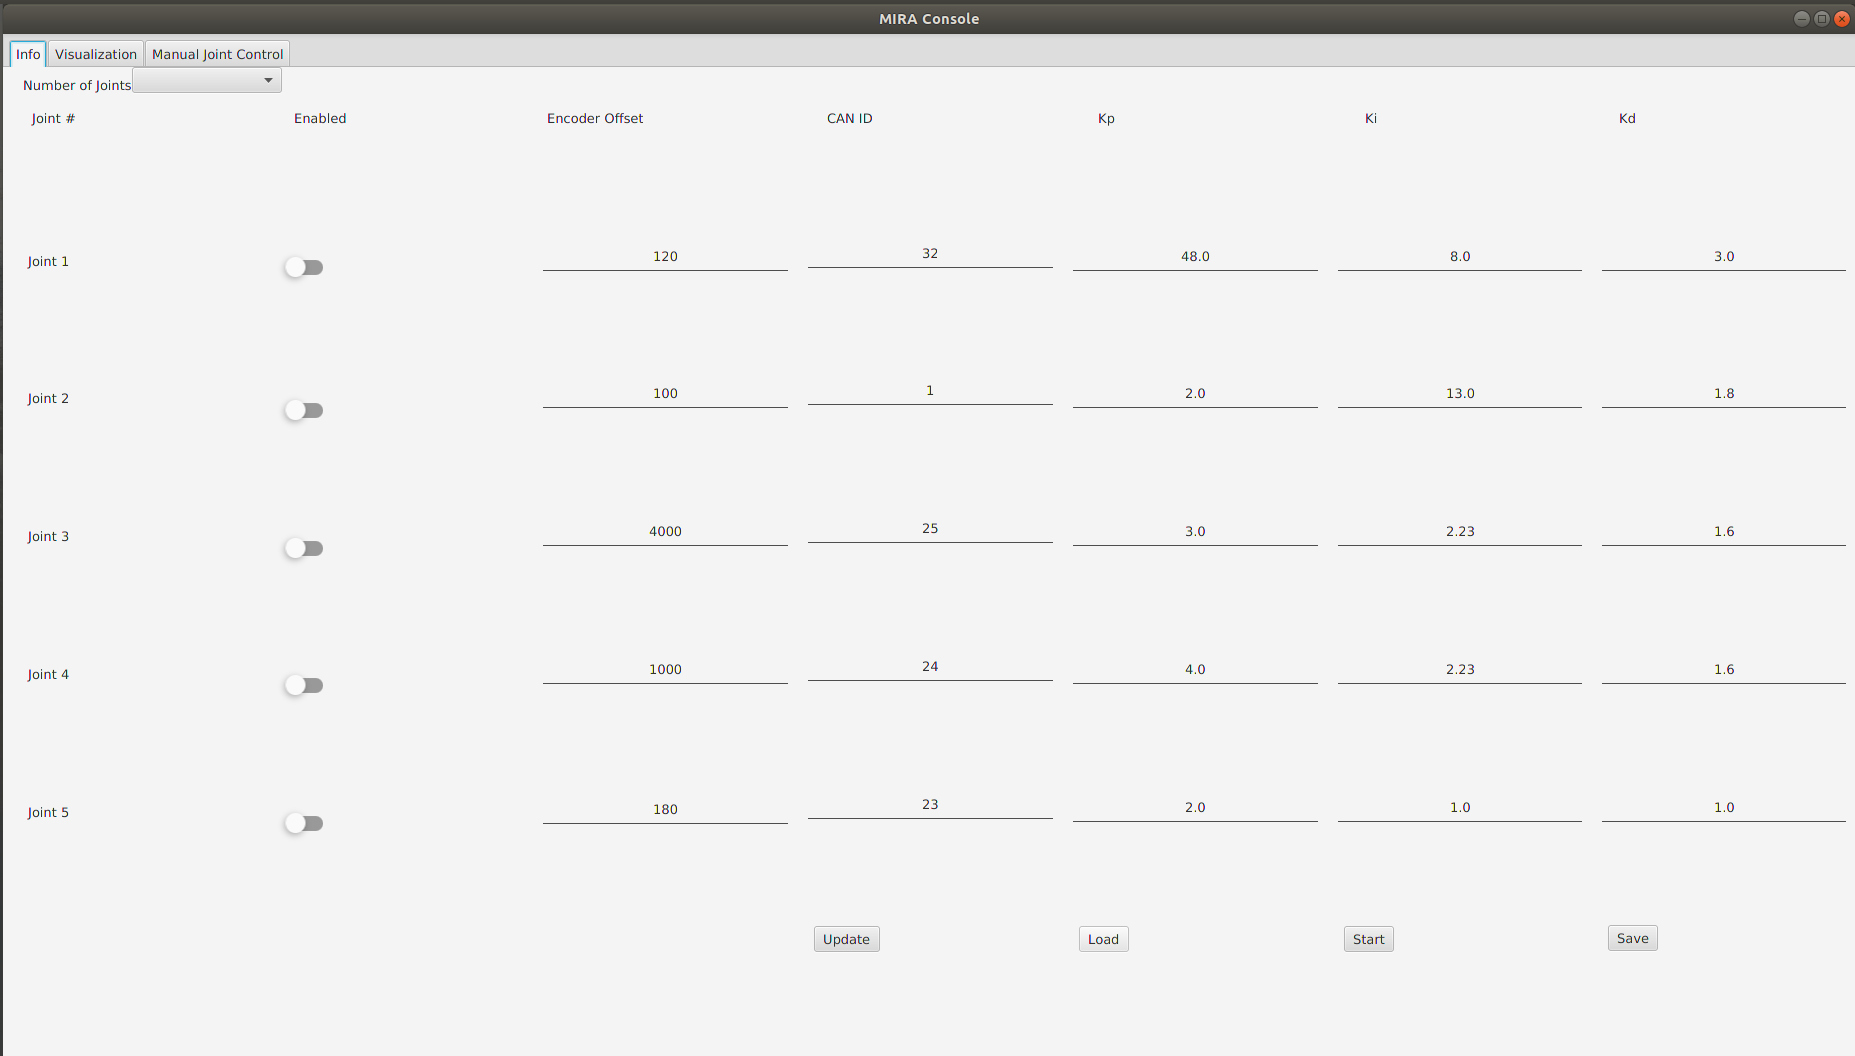
\includegraphics[width=\textwidth]{GUI_config}
	\caption{GUI config tab with save and loading}
	\label{fig:GUI_config}
\end{figure}







%\subfile{Chapters/Capstone_Reqs}
%\subfile{Chapters/Constraints}
%\subfile{Chapters/Acceptance_Criteria}
%\subfile{Chapters/Test_and_Validation}
\section{Testing}
\subsection{Acceptance Criteria}
% Section outline
% Overall summary of section, list of deliverables
Acceptance criteria for this project will be broken into 5 major categories: Joints, End effector, Base, Software application, Code library

\subsubsection{Joint Board}
\begin{itemize}
	\item Receive initialization information and joint angles from base
	\item Moves joint to angles
	\item Send position updates back to base
	\item Pass power and signal buses
	\item Capable of powering logic without powering motors
	\item Control board is the same for each joint
\end{itemize}

\subsubsection{Modify RBE3001 Arm}
\begin{itemize}
	\item Remove control system and replace with our own 
	\item Add a link to the existing arm
	\item Replace currently implemented servo motors with brushed DC motors
\end{itemize}

\subsubsection{End Effector}
\begin{itemize}
	\item Receives power and signal buses
	\item Keyed connection
	\item One input connector
	\item Terminate CAN bus
	\item Uses a joint board
\end{itemize}

\subsubsection{Base}
\begin{itemize}
	\item Sends and receives joint angles to/from Personal Computer (PC)
	\item Receives initialization information from PC, then sends it to all joints on signal bus
	\item Outputs power and signal buses
	\item Converts AC wall power to system power bus
	\item Power supply and arm on/off switch
	\item Capable of powering logic without powering motors
	\item Array of indicator LEDs
\end{itemize}

\subsubsection{Software Application}
\begin{itemize}
	\item Sends configuration information to the Code Library
	\item Sends individual joint angles or pose commands to robot through the Code Library
	\item GUI to adjust current arm configuration parameters
	\item Record and play back sequence of poses
	\item Acts as a front-end for code library
	\item Stretch goal: 3D model of arm moving in real-time
\end{itemize}

\subsubsection{Code Library}
\begin{itemize}
	\item Receive configuration information from user, selects control constants, sends to base
	\item Able to control the robot: Receive joint status, send joint angles
	\item Calculate joint angles using kinematics
	\item Stretch Goal: Written so that it can interface with multiple languages
\end{itemize}

\subsection{Motor Driver}
In order to determine whether the performance of the motor driver was dependent on input frequency or other factors, the input frequency was increased again from 200Hz to 10kHz. This time, the motor performed much better than previous times where it stayed at a constant RPM at different frequencies. The RPM actually increased with an increase in frequency, as can be seen in Table \ref{tbl:freq-test}. With this in mind, we decided to use a PWM frequency of 1KHz.
%insert table of input frequency vs motor rpm
\begin{table}[H]
	\centering
	\caption{PWM frequency input at 50\% duty cycle vs motor speed}
	\begin{tabular}{| c | c |}
		\hline
		PWM Frequency (Hz) & Motor RPM (rpm) \\
		\hline
		200 & 80 \\
		400 & 79 \\
		1k & 81 \\
		2k & 82 \\
		5k & 86 \\
		10k & 90 \\
		\hline
	\end{tabular}
	\label{tbl:freq-test}
\end{table}


%\subsection{Demultiplexer}
%
%\subsection{INA332}
%In order to generate a small input voltage to the amplifier, a potentiometer was used with a larger resistor in series, creating a variable voltage divider. To create the small input voltage necessary, a 100k$\Omega$ resistor and a 1k$\Omega$ potentiometer were used. With the configuration given in \ref{sec:meth-ina332}, the expected
%
%\subsection{TM4C123}
%Several peripherals were needed to achieve the desired functionality from our microcontroller. A test board was set up in order to test and verify that each of these peripherals was setup properly and working as expected. The test board consisted of a potentiometer connected to an ADC pin, an SPI controlled ADC (MCP3202), the 1:2 demultiplexer (SN74LVC1G18), CAN transceiver (TC332), and some LEDs.
%
%As a temporary stand in for the AS5055 absolute Hall effect encoder to test the SSI peripheral, a MCP3202 12-bit, 2 channel ADC was used. Both devices use SPI to communicate their sensor data back to the MCU, and the packets are similar in structure. Some differences between the two that can be changed are a maximum sample rate for the AS5055 of ~1ms as opposed to the few SCLK cycle delays for the MCP3202. The AS5055 has a maximum SCLK frequency of up to 10MHz at 3.3V while the MCP3202 has a limit of 900kHz at 3.3V.
%
%The potentiometer was connected to PB? which was enabled at AIN3. The ADC was set to sample at 1kHz with hardware oversampling 16x enabled.
%\subsection{Hall Effect Encoder}
%\subsection{CAN Bus}
%Initial CAN testing consisted of

% \subfile{Chapters/Conclusion}
%TODO Recommendations for future work
%TODO Table of acronyms
\pagebreak
\bibliographystyle{ieeetr}
\bibliography{export}{}

\begin{appendices}
%\section{Kit Components}
\label{app:KitParts}
\begin{itemize}
\item 3x Twist Joints
\item 3x Revolving Type A Joints
\item 3x Revolving Type B Joints
\item 3x 75mm Links
\item 3x 150mm Links
\item 3x 225mm Links
\item 1x Claw Gripper End-of-Arm Tool
\item 1x Hook End-of-Arm Tool
\item 1x Capacitive Stylus/Pointer End-of-Arm Tool
\item 1x Master Controller
\item 1x Power Supply Unit
\item Stretch Goals:
\begin{itemize}
\item Prismatic Joint(s)
\item 1x Universal Gripper End-of-Arm Tool
\end{itemize}
\end{itemize}
%\section{Gantt Chart}
\label{app:Gantts}

\begin{figure}[H]
\centering
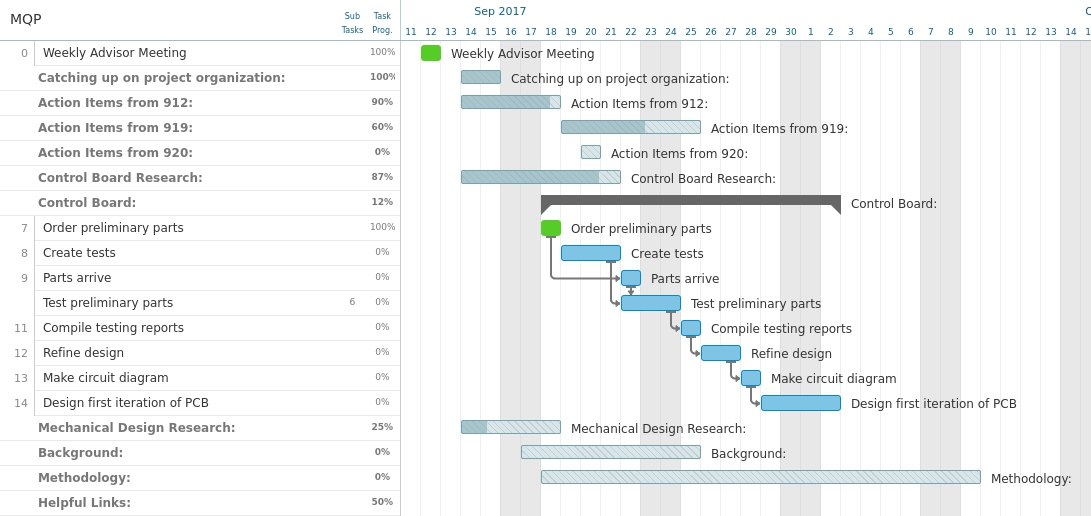
\includegraphics[width=\textwidth]{Gantt_Control_Board}
\caption{Gantt chart for project focused on the Control Board}
\label{fig:gantt}
\end{figure}
\pagenumbering{arabic}% resets `page` counter to 1
\renewcommand*{\thepage}{A\arabic{page}}
\section{Early Project Iteration}
\subsection{Introduction} 
% Section outline:
% Overall summary of project - ~1 sentence per major goal
% ~1 Paragraph for each major goal
% Paragraph at end describing what is in this document

The goal of this project is to create a cost-effective, modular kit of parts that can be used to create a robotic arm. In this paper, we will be using the word "Joint" to refer to a piece of the arm that has a motor, and we will use "Stick" to refer to the part of an arm that connects two joints. The joints provide degrees of freedom for the arm while the sticks space out the joints. Joints can connect to joints and sticks, but sticks can only connect to joints. End-of-arm tools can be swapped out, but not during operation. In addition to a physical kit, we will create a GUI for easy configuration and basic control of the arm. The base will communicate with a computer running control code either through the software application or code library. \\
\newline
We aim to construct our kit with smart joints and dumb sticks. This will be accomplished by designing a controller board that has all the necessary components to control one motor. This controller board will be placed on each joint and connected to a main processing unit in the base that handles control for the entire arm. The full set of components for this kit are outlined in Appendix \ref{app:KitParts}.\\
\newline
We will create a software application to interface with a constructed arm. The user will input how they have constructed their arm into this application and then be able to do some simple control. Another feature of this application will be the ability to record a series of poses for the arm to perform. In addition to this software, we will also create some programming libraries to allow users to control the arm with an actual program. \\
\newline
In this document, we will outline some existing robot arms and highlight the differences between these arms and our arm kit. Next, we discuss what work there is to be done on this project. After discussing the work to be done, we will state how this work will satisfy the capstone design requirements for each of the three disciplines represented by our group members. Then, we state the constraints we expect going forward with this project. Next, the acceptance criteria for any deliverables at the end of this project will be outlined. Finally, we will state an estimated timeline for this project.

\subsection{Background}
% Section outline
% Overall summary of section - ~1 sentence per major topic
% ~1 Paragraph for each major topic
This section begins with an overview of some existing robotic arms that are about the same size as a fully assembled arm from our kit will be. Next we discuss some existing modular robotic arms. Finally, we highlight how our kit will be different from the discussed prior art.

\subsubsection{Robot Arms Currently in Use}
There are a plethora of industrial robotic arms. Since our kit will be relatively small compared to most industrial arms, we will begin with an overview of existing desktop industrial arms. Arms that fit this description have a reach of less than 1000mm. Industrial robot arms typically cost between \$50,000 and \$80,000 new and \$25,000 and \$40,000 used \cite{RobotWorx}. Some manufacturers of these industrial arms include ABB Robotics, Universal Robots, and KUKA Robotics. It's important to note that none of these arms are modular - in fact, they can't be changed at all!

\subsubsubsection{ABB Robotics}
ABB Robotics makes many small industrial arms. The ABB IRB 120 boasts a 580mm reach, 3kg payload, and 25kg weight. It has 6 degrees of freedom and can be mounted at any angle. The ABB IRB 1200 comes in two varieties, one with a reach of 703mm reach and 7kg payload, and one with a 901mm reach and 5kg payload. Both of these arms have 6 degrees of freedom. The weights are similar at 52kg and 54kg respectively \cite{RobotWorx}.

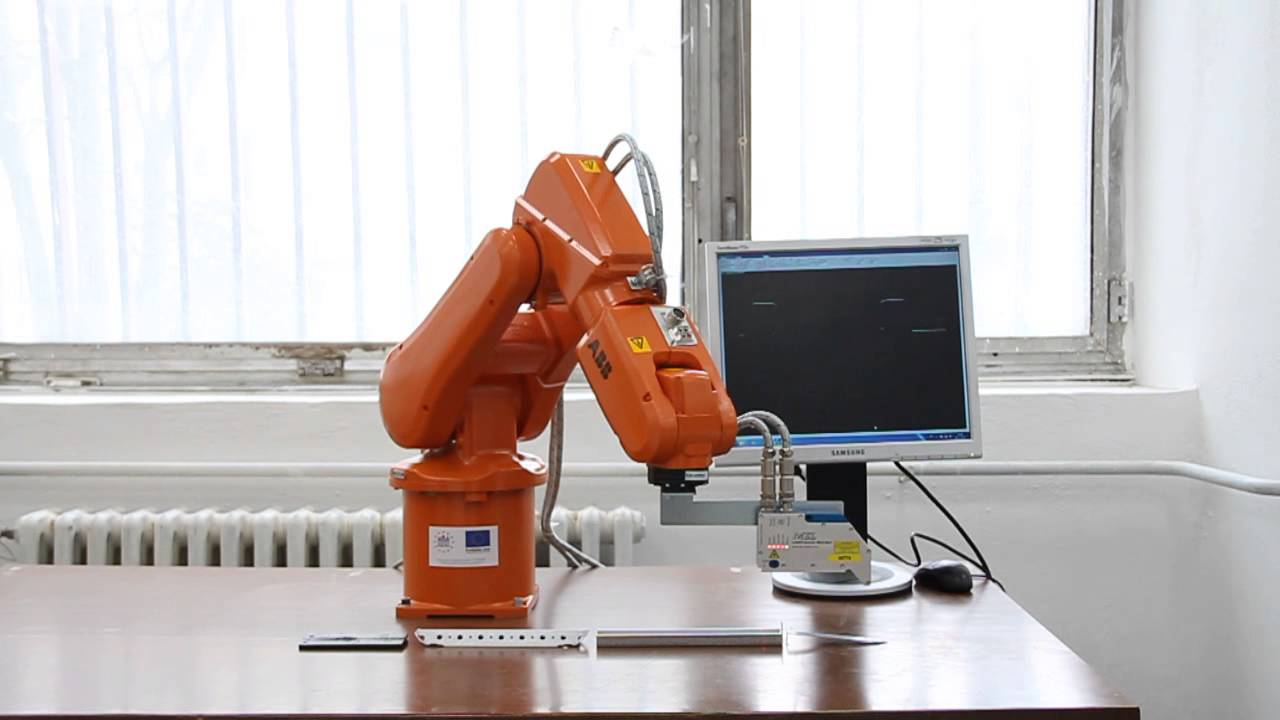
\includegraphics[width=\textwidth]{ABB-irb-120}
\cite{IRB_120}

\subsubsubsection{Universal Robots}
Universal Robots makes two robot arms in this size range. The UR3 is the smaller of the two with a reach of 500mm, payload of 3kg, and 11kg weight. A step up is the UR5 which has a 850mm reach, 5kg payload, and 18.1kg weight. Both of these arms have 6 degrees of freedom. Universal boasts that these arms are easy to implement and re-implement due to compact and lightweight construction, and simple programming interface \cite{RobotWorx}.

\subsubsubsection{KUKA AG}
KUKA makes two robot arms in this size range. The KR3 R540 has a reach of 541mm, payload of 3kg, and weight of 26kg. It can be mounted on the floor, wall, or ceiling for added utility. The K5 sixx R650 is larger with a reach of 650mm, payload of 5kg, and weight of 127kg. It can only be mounted on the floor or ceiling. Both of these arms have 6 degrees of freedom \cite{RobotWorx}.

\subsubsection{Small Industrial Robotic Arm Comparison}
Table \ref{tab:ArmComparison} shows a comparison of all the robotic arms discussed in this section.
\begin{table} [H]
	\centering
	\begin{tabular}{| l | c | c | c | c |}
		\hline
		\textbf{Name} & \textbf{Reach (mm)} & \textbf{Payload (kg)} & \textbf{Weight (kg)} & \textbf{Axes} \\
		\hline
		IRB120 & 580 & 3 & 25 & 6 \\
		IRB1200-7/0.7 & 703 & 7 & 52 & 6 \\
		IRB1200-5/0.9 & 901 & 5 & 54 & 6 \\
		UR3 & 500 & 3 & 11 & 6 \\
		UR5 & 850 & 5 & 18.1 & 6 \\
		KR3 R540 & 541 & 3 & 26 & 6 \\
		K5 sixx R650 & 650 & 5 & 127 & 6 \\
		\hline
	\end{tabular}
	\caption{Comparison of $<$1000mm reach industrial robot arms}
	\label{tab:ArmComparison}
\end{table}

\subsubsection{Modular Arms}
While there are many industrial arms in production, there are very few modular robotic arms. There is one commercially available robotic arm, the Robolink, made by igus. A few modular robot arms have been developed, including the reconfigurable modular manipulator (RMM), made by TRACLabs \cite{RMM}, and a single joint for the Modular Robotic Arm project MQP at WPI \cite{MRA}.

\subsubsubsection{igus Robolink} 
Robolink is a modular robotic arm kit produced by the plastics manufacturing company igus.  The kit contains parts to make an arm that is up to 6 Degrees of Freedom (DOF), with belt driven linkages powered by stepper motors that reside in the base of the robot.  Robolink offers 7 individual links, ranging from 1-2 DOF and differing based upon their kind of motion (pivoting, rotating, swiveling).  Each link is made of a lightweight and strong plastic or carbon fiber with cables inlaid in them, resulting in a low cost and weight arm.  The cables used to control these links are made of a high strength synthetic fiber with has a tensile strength of 4,000N.  Separating the actuation of each link from the joint allows the arms to be easily maneuverable with its lightweight and strong joints.  \\
\newline
Purchasers of the kit are able to combine the links in different ways, allowing for a flexible, modular solution to robotic arms. Igus also offers their Robolink software for programming articulated arms that facilitates the programming of individual arms through the use of a simple, intuitive control software. The total cost of a kit to make a 6 DOF arm is \$6000, and buying individual links will cost anywhere from \$370 to \$750 per link. While this price may be low cost compared to other arms such as the ABB robotic arm which can cost up to \$200,000 in total, it is still not low enough for either hobbyists or people interested in learning about robotic arms who are prevented from doing so by the high entry cost. In addition to this, the belt system actuating each link requires the user to thread belts attached to the actuators to each link in order to set up the robot. The long assembly time and intricacy also detracts from the idea of modularity because the time involved in switching configurations can inhibit users from really exploring the different workspaces and combinations this kit can create \cite{igus}.  

\subsubsubsection{Reconfigurable Modular Manipulator}
The reconfigurable modular manipulator developed by TRACLabs for NASA is a fully modular 7-DOF robot arm. Each joint and end effector have the same connector that provides power and control lines throughout the arm. Internal power and control circuitry take in these lines and convert them into movement. Joints can be swapped out by hand in a matter of seconds. Joints accept position or velocity data from the central communication lines and store physical characteristics about the joints in memory. This robot arm is not commercially available \cite{RMM}.

\subsubsubsection{Modular Robotic Arm}
This project aimed to close the market gap between inexpensive toy robot arms and expensive professional grade industrial arms. The group aimed to do this by designing a single joint that could be used to assemble a robot arm. Ultimately, a single DOF joint that was heavy, difficult to manufacture, and expensive to produce was designed and constructed. In their future recommendations section, the group stated that the goal of designing a modular robot arm was possible but their design was not the solution \cite{MRA}.

\subsubsection{Our Robotic Arm System}
Our modular robotic arm kit aims to offer a completely different experience compared to existing products and projects. The system maintains a low cost while providing a versatile platform for beginner engineers or rapid prototyping professionals. This is achieved by avoiding expensive proprietary software and subtractive manufacturing; favoring off-the-shelf parts, 3D-printed structures, and freely available software. Providing custom-built software for controlling the arm creates a plug-and-play environment suitable for most any skill level.

% \subsection{Communications}
% We looked at several types of communications for the purposes of controlling our robotic arm. These include serial UART, SPI, I2C, and CAN. 
% \subsubsection{Controller Area Network}
% A controller area network (CAN) is a system for sending data reliably between distinct subsystems with reasonably low danger of transmission errors. CAN buses are widely used in the automotive industry to allow various computerized parts of the car to talk to one another.

% Research begins here?
\subsubsection{Control board}
The control board is meant to be implemented as an independent module that interfaces with a main controller module. Its tasks are to send and receive data from the main controller and control the position of a single motor. As such, the main factors that must be taken into account when designing the control board are methods of measuring joint position and motor torque, as well as communicate with an off-board controller. Motor torque is proportional to motor current. Therefore, the motor torque will be calculated from the measured current through the motor.

\subsubsubsection{Joint Position Detection}
Angular position sensing must be used to determine the joint angle of the motor. There are several commonly used methods of determining angular position, including potentiometers, optical encoders, and hall effect sensors \cite{Pot_vs_Sensor,Choose_Sensor_Technology,Choose_Position_Sensor}. A comparison of the different angular sensors can be seen in Table \ref{tbl:Angular_pos_sensors}. \\
\newline
Potentiometers are very commonly used to measure angular position due to their simple implementation and low cost. In addition to being low cost, potentiometers provide high linearity and accuracy \cite{Choose_Position_Sensor}. Although generall robust, these sensors do not lend themselves well to many, rapid adjustments or mechanical vibrations. Both of these significantly reduce the lifespan of the sensor \cite{Pot_vs_Sensor,Choose_Position_Sensor}. The situations potentiometers excel in are those that require an easily adjustble voltage at low to medium adjustment frequencies, such as settings nobs on control panels or analog reference voltages as trim potentiometers \cite{Pot_vs_Sensor}. \\
\newline
Hall Effect sensors are less commonly used, and consist of a bipolar magnet rotating above a hall effect sensor with the axis of rotation perpendicular to the plane of the sensor. Since there is no contact between the rotation and the sensor, these types of sensors have very long lifespans \cite{Pot_vs_Sensor}. Unfortunately, these sensors do not provide high resolution since they are susceptible to electromagnetic interference and tempterature, and also have some hysteresis \cite{Choose_Position_Sensor}. \\
\newline
Optical encoders are another method of measuring angular position. These sensors consist of a beam of light that shines on a slotted disk so that as the disk rotates, the slots break the light beam. These sensors can have very high resolutions and are resistant to shock and vibrations \cite{Choose_Sensor_Technology}. Like magnetic sensors, these sensors have very long lifespans since there is no mechanical connection on the sensor \cite{Pot_vs_Sensor}. Unfortunately, these sensors are susceptible to foreign particles blocking the light beam from sensing the slots and causing incorrect readings. The most common kind of optical encoder, the Quadrature encoder, does not sense absolute position; it can only read relative position, meaning that a quadrature encoder would need to be combined with some other sensor in order for the robot to be able to sense its joint angles correctly. Other encoders called Absolute Encoders do not have trouble reading absolute position, but they are prohibitively expensive. \cite{Choose_Position_Sensor}. 

\begin{table}[H]
	\begin{center}
		\begin{tabular}{ | p{2.4cm} | r | p{1.6cm} | l | l | p{2.5cm} |}
			\hline
			Sensor & Cost & Linearity & Accuracy & Lifespan & Notes
			\\ \hline
			Potentiometer & \$ & Depends on ADC & Moderate & Short & Repeated motion at the same angle can lead to failure
			\\ \hline
			Encoder & \$\$\$ & Very High & Very High & Long & Cheap ones can't sense absolute position
			\\ \hline
			Hall Effect Sensor & \$\$ & High & High & Very Long & Requires special attention to surrounding magnetic fields when mounting
			\\ \hline
		\end{tabular}
	\end{center}
	\caption{Comparison of different angular position sensors}
	\label{tbl:Angular_pos_sensors}
\end{table}

\subsubsubsection{Current Sensing}
Current sensing can be done in many ways. The most common way is by using a shunt resistor and an amplifier. A variant of this method is to use the resistance inherent in the wires or traces as a shunt resistor. Another common method of current sensing is to use a hall effect sensor \cite{Current_Sensing}. \\
\newline
Shunt resistors are used in either high side or low side configuration. They are simple to integrate, low cost, and capable of measuring both AC and DC currents. The downsides to this method are relatively large insertion loss that increase exponentially with current, large thermal drift that must be compensated for, as well as large system noise from amplification. There are two main implementations of shunt resistors, high side and low side \cite{Current_Sensing}. \\
\newline
Low side current sensing means that the shunt resistor is placed in the return current path. This method is simpler to implement since the voltage on the shunt resistor is with respect to ground, so it can simply be amplified. Some problems exist with this, however, since the resistor seperates the current path from ground. In this configuration, the circuitry used to measure the voltage on the shunt resistor will not report a fault if the sytem experiences a short circuit \cite{Current_Sensing}. \\
\newline 
High side current sensing means that the shunt resistor is placed on the forward current path. This configuration is able to detect short circuit faults, an advantage to using this configuration over low side current sensing. An additional advantage is that the return current path is directly connected to ground. The downside to high side current sensing is that it requires a differential amplifier since the voltage across the shunt resistor is very close to supply voltage. \cite{Current_Sensing}. \\
\newline
Trace resistance sensing is very similar to using a shunt resistor, but there are some slight differences. Since there isn't a way to control the resistance of a copper trace, the system must be calibrated after being assembled. Another key difference is the amount of amplification needed. Copper traces have very low inherent resistance, so a very large amplification must be used. This large gain imposes a limitation on the maximum measurable bandwidth set by the gain bandwidth product of the amplifier \cite{Current_Sensing}. \\
\newline
Hall effect sensors are commonly used to measure current as well. These sensors can measure current intrusively or non-intrusively, as well as in open loop or closed loop configurations. Non-intrusive devices measure current by wrapping wire around a toroid that focuses the magnetic field on a sensor in a break in the ring of the toroid, or placing the hall effect sensor on top of the current to be measured. These work fairly well, but are very susceptible to noise from magnetic fields upwards of 10cm away. Methods of shielding these sensors exist, but are complicated and expensive to implement. Intrusive sensors route current through the device and measure the generated magnetic field with a hall effect device near the current path. Open loop applications take the voltage generated on the hall effect sensor and condition it to whatever output is needed. Closed loop sensors reroute the sensed current to a secondary coil that is used to generate a proportional current to the measured current. This proportional current is then used as feedback to reduce error \cite{Current_Sensing}. \\
\newline
Insertion loss caused by these sensors is very small. Since these sensors measure current by induction, they can only measure current in a specific frequency band, and high currents at high frequencies can cause these devices to overheat. Most of these frequencies are DC to some upper limit determined by the physical characteristics of the sensor, usually around 100kHz. These sensors cannot be used on their own, since they have an inherent voltage offset, called misalignment voltage, and suffer from high thermal drift. Integrated ICs that compensate for these factors are fairly widespread, allowing for very easy integration \cite{Current_Sensing}.

\subsubsubsection{Off-Board Communication}
There are many types of communication protocols that could be used to communicate with the main controller. Common protocols include SPI, I$^2$C, RS232, RS485, and CAN. Of these, SPI and I$^2$C are meant mostly for chip to chip communication while RS232, RS485, and CAN are all meant for module to module communication \cite{SerialCompared}. A comparison of these protocols can be seen in Table \ref{tbl:Comm_Compare}. \\
\newline
SPI is a full duplex, synchronous serial link consisting of 3 lines, SCLK, MOSI, MISO, and an additional line for every peripheral, CS. Data rates of up to 10MHz or more are possible due to the elimination of addressing with the CS lines and dedicated clock line \cite{SerialCompared}. Using SPI for controller-to-controller communication presents a problem, however. Since the data transfer rate is controller by the master, the slave could fall behind on processing data. This can be avoided by only transmitting data one direction at a time. Typically, SPI is limited to onboard communications since its signal degrades fairly quickly over distance \cite{CANvSPI}. \\
\newline
I$^2$C is a half duplex, synchronous, multi-master bus consisting of a clock and data line. Data rates of up to 3.4MHz can be reached, and each device has a unique address or multiple addresses to avoid overlap. An interesting aspect of I$^2$C is clock stretching. Clock stretching is when a slave pulls the clock low to stall the master until it has enough time to process information. Typically, I$^2$C is limited to onboard communication since its signal degrades fairly quickly over distance \cite{SerialCompared}. \\
\newline
RS232 is a common full duplex interface that consists of two transmitter/receiver pairs. The protocol limits communication to 1 sender and 1 receiver per line. Data rates of up to 115.2KHz are possible at a range of up to 200ft. Data is typically sent in 8N1 format with 8 data bits, no parity bit, and 1 stop bit or 7E1 format with 7 data bits, even parity bit, and 1 stop bit \cite{SerialCompared}. \\
\newline
RS485 is a full duplex multi-master protocol that consists of up to 32 transceivers on the bus. Data transmission rates of up to 10Mbps and distances of up to 4000ft are possible. Transmission can be reduced to half duplex by removing one transceiver at each node. Data is sent much the same as in RS232 with either 8N1 or 7E1 being common formats \cite{SerialCompared}. \\
\newline
CAN is a half duplex multi-master bus protocol that allows for many nodes to connect and send data on the two transmission lines. Messages are sent with unique addresses that also act as arbitration for bus priority. Packets are fully defined with 11 or 29 bit addresses, 0-8 bytes of data, and some additional control and verification bits \cite{CAN_Guide,CAN_Requirements}. Data rates of up to 1MHz and distances of up to 3000ft are possible. Multiple error checks are implemented at the hardware level since packets are predefined, allowing the controller to load a transmit buffer and let the transceiver send a message or wait until a receive buffer is full before reading the message \cite{CANvSPI}. 

\begin{table}[H]
	\begin{center}
		\begin{tabular} {| l | l | p{2cm} | p{2.5cm} | p{2.5cm} |}
			\hline
			Protocol & Max Distance & Max Speed & Wires needed & Notes \\ \hline
			SPI & Within circuit board & 10MHz & SCLK, MOSI, MISO, + 1 CS for each node & No addresses needed
			\\ \hline
			I$^2$C & Within circuit board & 3.4MHz & 2 & Address included in message
			\\ \hline
			RS232 & 200 feet & 115.2KHz & 4 & Can include parity bit
			\\ \hline
			RS485 & 4000 feet & 10Mbps & 4 & Can transmit fast or far but not at same time
			\\ \hline
			CAN & 3000 feet & 1MHz & 2 & Resilient signal
			\\ \hline
		\end{tabular}
	\end{center}
	\caption{Comparison of off-board communication protocol performance}
	\label{tbl:Comm_Compare}
\end{table}

% \begin{figure}[H]
% \centering
% \includegraphics[width=\textwidth]{Detailed_Block_Diagram}
% \caption{Functional block diagram of the system}
% \label{fig:Functional_Block_Diagram}
% \end{figure}

\subsection{Description of Work}
% Section outline
% Overall summary of section - ~1 sentence per major topic
% ~1 Paragraph for each major topic

% What work is there to be done?
There are many different ways to accomplish the goals we set. We decided to design several "smart" joints, "dumb" sticks of various lengths that passes signals through from joint to joint, changeable end of arm tools, a base for routing messages to each joint as well as providing power to the entire system, and a computer for performing complex real-time calculations. We plan to design every component listed in the kit of parts found in Appendix \ref{app:KitParts}. \\
\newline
We decided on designing two different joints (twist and rotation), with keyed connectors so they can connect in one of four orientations. Two kinds (straight and right angle) and three different lengths (75mm, 150mm, 225mm) of sticks will be designed as well. Joints can connect to sticks and joints, but sticks can only connect to joints. As such, the connectors will have to be designed with this in mind. Each connector will have to make a strong physical connection as well as a solid electrical connection to send power and data through to each Joint. \\
\newline
Each joint will have a control board that allows it to connect to the main communications line running through the system and control the motor on the joint. This board will have all of the necessary components for controlling one motor and communicating with the base. The base will act as an interface between the computer that is performing all of the complex calculations and the joints that are controlling their positions. The computer will need to have a USB port and be able to run Python programs.\\
\newline
We will develop some software for controlling the arm with a GUI that will run on the user's computer. This software will have a simple control interface for moving the arm, and some configurable settings to act as inputs for the kinematics equations. In addition to this we will develop a code library for end users to interface with in their own code.

\subsection{Methodology}
\subsubsection{Kit Components}
We decided to break a robot arm down into its component parts. We came up with the main parts of our kit: sticks, joints, a base, and end of arm tools. This breakdown was to try to maximize modularity while keeping the pieces relatively simple. By separating the joint from the stick, we can have multiple sticks, which are easy to manufacture, of different types and lengths to offset a few types of joints, which are difficult to manufacture. The base is necessary to send and receive computation control from a computer. Multiple end of arm tools are needed to provide functionality to the arm besides movement.

\subsubsection{Connectors}
The connectors are vitally important to the functionality of this project. A good connector will need to make solid mechanical and electrical connection between parts while also providing the ability to quickly connect and disconnect parts. In addition, the type of connection we choose will affect the modularity of the system as a whole. The important things to note while deciding on criteria for the connector are how/if they will be keyed, how they will pass electrical signals, where exactly the connector will be on the joints, and how the connector will be secured.

\subsubsubsection{Connector Position on Joints}
Connector position is the first major design choice we had to make. They can be positioned either on the axis of rotation of the joint or off the axis of rotation of the joint, and selecting one method versus the other vastly changes the way that the connector would work. Putting the connector ON the axis of rotation means that the connector would connect to the joint axis directly, while putting it OFF the axis of rotation means the connector would connect to a piece that is connected to the joint axis. \\
\newline
The advantage that placing the connector off the axis of rotation has over placing the connector on the axis of rotation is that the joint will be a solid unit. Having the joint be a solid unit seems a better design choice than splitting it in half, so we decided to go with putting connectors off the axis of rotation.

\subsubsubsection{Securing the Connection}
%available options: no tools, single screw, multiple screws, slots with removable pins
One of the important aspects of a modular system is how easy it is to connect or disconnect parts to or from that system. The main options for quick connections are requiring no additional hardware, requiring a single screw, and requiring slots and pins. \\
\newline
The most obvious solution is to connect parts with no additional hardware required. This creates a very complicated design challenge since using no tools means the user would have to secure any connection with just their hands. This can weaken the joint mechanically. The advantage to this method has is that it is fairly quick. \\ 
\newline
A step down in the simplicity solution is to require a single screw to join two pieces together. This is still simple and pieces can be connected somewhat quickly, but does require a tool to connect pieces. The main advantage is that screws hold parts together very well and the mechanical integrity of the connection should be held. \\
\newline
Another option is to design the joints and sticks in such a way that they slot together and are held in place with pins. This requires additional hardware, but no tools. This should keep pieces together fairly well while still allowing connections to be made quickly and easily. \\
\newline


\subsubsubsection{Keying the Connector}
Keying the mechanical connection between joints, sticks, and the base changes how modular the system is overall as well as how many unique components will be needed in each kit. Not keying the connection is not an option since this would allow the user to connect the pieces together in any orientation and the orientation needs to be known in order to accurately control the arm. This leaves two main options for the connections: keying for 1 orientation and keying for 4 orientations.\\
\newline
Keying the connectors for 1 orientation means that three different kinds of revolute joint must be design to fully represent the ways a revolute joint can move in 3D space. Essentially, this would mean each different joint would rotate about a different axis relative to the connector axis. The modularity of the kit is impacted quite negatively by doing this, since each joint can only connect in one way and therefore cannot be used where another type of rotation is needed. This design is quite simple, however, since the connectors don't need to be rotationally symmetric about any axis. \\
\newline
Keying the connectors for 4 orientations presents a slightly more challenging design problem, however. The connectors would need to be evenly rotationally symmetric 4 ways about the axis of connection in order for this design to work. 4-way keyed connectors will bring the number of unique joints down from 3 to 2. Doing this does help with the modularity of the design, though, since the rotational joint can be implemented to rotate in either axis perpendicular to the connector axis. A disadvantage of this configuration is an increase in complexity. \\
\newline
Since additional complexity when designing is less important that the overall modularity, we decided to go with a 4-position keyed connection. This allows a single rotational joint and only 1 right angle stick design so that the user can construct many different kinds of arms from these simple parts.

\subsubsubsection{Passing Signals}
% rigid connectors on joints, wires running along outside, wires running through inside that pop out at connector
Connectors also need to pass the power and signal buses through from joint to stick or joint. This can be done in one of a few ways, including: rigid mechanical connectors, loose wires running along the outside of parts, wires running inside of parts, and wires connecting internal bus bars. \\
\newline
Rigid mechanical connectors for passing signals would make connection when parts are connected together. These connections would have to be evenly rotationally symmetric 4 ways about the axis of rotation since the mechanical connectors are. A disadvantage of these connectors is that they rely on the integrity of the mechanical connection to pass electrical signals properly. If the connection flexes or bends too much then the electrical connection could break even though the mechanical connection is still mostly intact. Another disadvantage is that this is the most costly option for passing electrical signals, requiring 4 connectors per connection. \\
\newline
Loose wires along the outside of the parts have several advantages over rigid mechanical connectors. The first of which is that they only require one set of connections per connector. This reduces the cost of each connector significantly. The main disadvantage of this kind of electrical connection is that the wires could get snagged on something since the system is supposed to be active and moving. Another disadvantage is that the wires need to have enough slack to move with the arm without limiting the arm's movement.  \\
\newline
Wires running through the parts that pop out at the connectors is another option or passing signals along the system. This option is practically the same cost as external wires, but doesn't have the problem of wires snagging on the environment. Unfortunately this doesn't solve the problem of wires needing lots of slack to allow for movement of the whole system. \\
\newline
Short wires that connect some internal bus bars provide a more expensive solution to this problem. This would remove the problem of wires needing slack for the entire system. Instead, wires would only have enough slack for one joint. Doing this does bring some complexity issues, however, since the bars would have to be designed into the system and not added on at the end. \\
\newline
For our design we decided to use internal wires running the length of the system. The low cost and simplicity of this solution outweighs the negatives of having to add lots of extra wire to account for movement of the system.\\

\subsubsection{Sticks}
%things to decide for sticks: material, lengths, types (straight, right angle)

Sticks are the things that connect joints together and space joints out. They do not have any electronics on board; they simply pass power and communication wires along to the rest of the arm. They need to be strong, light weight, and cheap.\\
\newline
Sticks have an input side and an output side. Two kinds of sticks will need to be created: one will be straight, and one will have a right angle at the input side.

\pagebreak

%yes I like this
%But it makes the page before look so awkward and sad. And it still puts the footnotes too high up


%The following defines two counter variables: startNum and runCount. Every time a new footnote is declared, we increment runCount by 1. Then, when we're populating the footnotes with words, we start with number startNum and count upwards.
\FPeval{\startNum}{(thefootnote)}
\FPeval{\startNum}{round((\startNum) + 1,0)}
\FPeval{\runCount}{\startNum}

\begin{table}[H]
	\begin{center}
		\begin{tabular}{ | l | l | p{1.5cm} | p{2.5cm} | p{2.5cm}| l |}
			\hline
			Stick Material & Cost/kg & Cost/ 20mm & Rigidity & Complexity & Weight \\ \hline
			3D-printed PLA\footnotemark[\runCount] & ~\$20/kg & \$3 & Might break  & Low: Very few constraints on possible designs & 150g \footnotemark[\runCount]
			\\ \hline
			\FPeval{\runCount}{round((\runCount)+1,0)}%
			
			PVC\footnotemark[\runCount] & \$7 & \$0.70 & Bends over time & Connect/ Disconnect easily & 106g\\ 
			\hline
			%I would have thought that the next line needed to add 1, not 2. My working hypothesis is that global variables can't really be modified from inside a table. I don't get it. Clearly the line is doing something, or else the \footnotemark line would simply do nothing.
			\FPeval{\runCount}{round((\runCount)+2,0)}%
			
			Carbon Fiber\footnotemark[\runCount] & \$66 & \$6 & Strong, but possibly too thin & & 58g\\ 
			\hline
			%I'm surprised that the next line adds 3 instead of 1. It works this way though. Oh well.
			\FPeval{\runCount}{round((\runCount)+3,0)}%
			
			80/20\footnotemark[\runCount] & \$2.46 & \$2 & Not going anywhere & Nice connecting options & 154g\\ 
			\hline
			%Only needed if more footnotes are added
			%\FPeval{\runCount}{round((\runCount)+1,0)}%
			
		\end{tabular}
		
	\end{center}
	\caption{Comparison of materials to construct sticks}
	\label{tbl:stick_materials}
\end{table}
\footnotetext[\startNum]{This number assumes 100\% infill. The actual number will almost certainly be lower.}
\FPeval{\startNum}{round((\startNum)+1,0)}

\footnotetext[\startNum]{\url{http://www.homedepot.com/p/Formufit-1-in-x-5-ft-Furniture-Grade-Sch-40-PVC-Pipe-in-White-P001FGP-WH-5/205171542?cm\_mmc=Shopping\%7cTHD\%7cG\%7c0\%7cG-BASE-PLA-D26P-Plumbing\%7c&gclid=Cj0KCQjwx8fOBRD7ARIsAPVq-Nlw\_xbuCOf-QHORvUW4gQ4Dx7SiZt\_vqQ3OvxBdTW-eckQhdp5WWFYaAs9DEALw\_wcB&gclsrc=aw.ds&dclid=CIagtKLB09YCFUuraQodN\_MAOQ}}

\FPeval{\startNum}{round((\startNum)+1,0)}

\footnotetext[\startNum]{\url{https://www.rockwestcomposites.com/45552?gclid=Cj0KCQjwx8fOBRD7ARIsAPVq-NmCNUg6ULxgd9udG-xSuPtJuHKgCLjUSgX\_zXPDgRr2CmKU0tSXX-waAgb9EALw\_wcB}}

\FPeval{\startNum}{round((\startNum)+1,0)}

\footnotetext[\startNum]{\url{https://8020.net/1010.html}}



We choose to use 3D-printed PLA. While it's not the absolute cheapest option, nor is it the lightest one, its high configurability makes it the ideal material for our needs - especially given its availability for potential customers; anybody with a 3D-printer would be able to make one of our arms. Also, while aesthetic concerns should not be the only factor, we're allowed to consider the way the final product would look. An arm made from PVC would reflect poorly on all the involved parties.


\subsubsection{Motor Selection}
\begin{table}[H]
	\begin{figure}[H]
		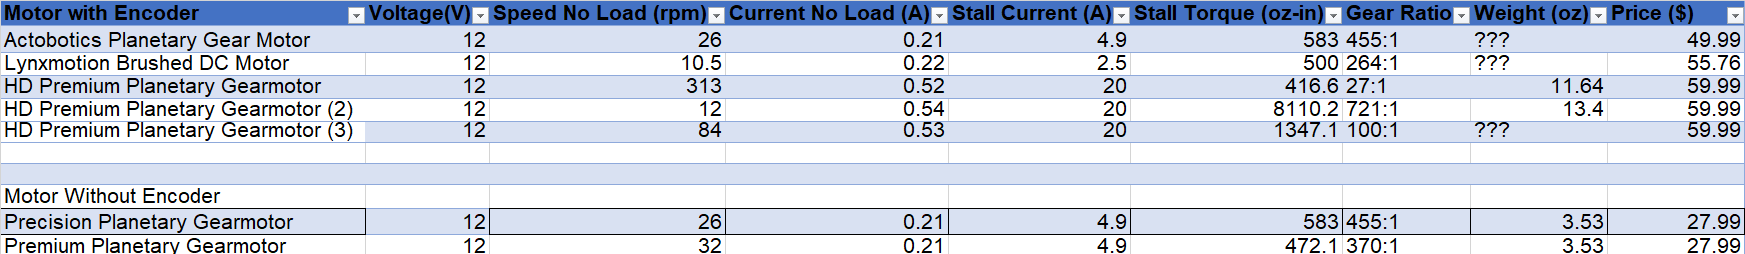
\includegraphics[width=\textwidth]{Pictures/motor_chart}
	\end{figure}
	\caption{Comparison of Possible Motors}
	\label{tbl:Motor_Chart}
\end{table}


To choose our motors, we looked for high-torque, low-cost DC motors. We chose to go with DC Brushed motors to control our arm because they are quiet, low-cost, vibration free and fairly efficient. We also considered using Dc Brushless motors as well as Stepper Motors, but each had their own pros and cons. Brushless motors cost much more than comparable brushed motors, and require complicated control logic to operate. Stepper motors were a good option due to their ability to be backdriven and their built in discrete steps for controlling. But, they do not operate well under conditions where the load changes significantly in a short period of time and also require external control to keep track of the position.  \\
\newline
Once we decided to use brushed DC motors, our next step was to find suitable motors that fit our criteria of high torque and low cost. We found 2 categories of motors that seemed to fill these requirements, planetary gearbox motors and spur gearbox motors. Planetary gearboxes work by having multiple "planet" gears revolving around a central "sun" gear that rotates in place. They are named for their resemblance of the planets orbiting around the sun. All of the "planet" gears are held in place by an outer "ring" gear that acts to keep the "planet" gears in contact with both the "sun" and the "ring". By having these idler gears rotating around a central axis, you can have torque transferred linearly, without the need for offset shafts, greatly reducing the total size of the gearbox. With multiple gears transferring the torque load at one time, the individual load on each tooth is lowered making these perfect for high torque applications. Spur gearboxes on the other hand use linear offset shafts that transfer the entire torque from one gear to the next until the output shaft in a direct chain.  This means that they wear out much faster since the torque load is much higher on individual gears and teeth.  Therefore, since we need a reliable high torque motor, we decided to go with planetary gear motors.  \\
\newline
Once we had made the decision to go with a planetary gearbox brushed DC motor, we made a chart as seen in Table 5 of possible motors that had high stall torques.  One final decision that we had to make was whether or not to purchase a motor with a rotary shaft encoder. Rotary shaft encoders provide easy control over DC motors by relaying the position of the shaft before the gearbox on the motor.  This allows for high resolution control in the case of high gear reductions but also costs a fair amount extra to purchase with the motor.  Considering that the motor is just a part of the joint and we care more about the position of the overall joint rather than the motor itself, we decided to save the money and go with a cheaper non-encoder motor.  By doing this we are moving the point at which we control the joint system from the motor to the joint if we use an absolute encoder on the joint shaft.  This results in a closed loop control system which is optimal for our situation and cost-effective.  

\subsubsection{Control Board Part selection}
Selecting the types of sensors to use for the control board was a very important step of the control board design. There are many different types of sensors to accomplish each major goal that the control board must accomplish.
\subsubsubsection{Joint Angle Sensor}
Potentiometers seem like a good choice due to their simplicity and high accuracy capabilities. However, they do not lend themselves well to this application because of how quickly they wear out. Over time, as the joints move to different positions, the potentiometers will wear out quickly and cause inaccurate readings. Additionally, long lifespan and high resolution potentiometers can be very expensive. Furthermore, potentiometers are large and can be difficult to mount. Finally, the hard stop on the potentiometer means the joint angles will be limited to a certain range (typically about 270 \textdegree  for single turn potentiometers).\\
\newline
The next obvious solution is to use optical encoders because they will not wear out and offer very high resolution capabilities. These sensors are not well suited for this application, however, since they are typically expensive, especially for high resolution encoders - and ones that are capable of reading absolute position. Additionally these sensors are somewhat bulky and would take up too much space in the closed environment of a joint. \\
\newline
This leaves us with hall effect sensors. These sensors are very small and moderately high resolution while also being a contact-free sensor, so wearing them out will not be a concern. A main concern with hall effect sensors is that they need to be mounted somewhat precisely and carefully. Traditional machining methods make this difficult to accomplish, but 3D printing allows us to easily overcome this challenge.  Another concern is external electromagnetic interference, but with somewhat careful circuit board design, we should be able to minimize this issue.

\subsubsubsection{Motor Current Sensor}
A shunt resistor seems practical due to the simplicity of the design, but careful designing must be done in order to get the noise levels down to a reasonable amount. In addition to this, the power loss when using a shunt resistor could cause the arm to stall before anticipated. When the shunt resistor takes power from the motor, the whole motor curve slides inward, decreasing the maximum power output. Trace resistance would be a good alternative, but requires calibration after the circuit is constructed. \\
\newline
Instead of these, we decided to use a hall effect current sensor. Hall effect current sensors are ready-made sensors that give low noise, properly calibrated outputs, are not very expensive, and are easy to integrate into a circuit design. These sensors have extremely small power losses to the motor. The main drawback of these sensors is that they have a low bandwidth, but we are using DC motors so this should not be a problem. Some care will need to be taken when placing these on the circuit, however, since they are sensitive to external magnetic fields.

\subsubsubsection{Off-board Communication}
SPI and I$^2$C are mostly used for on-board, controller-to-peripheral communications and therefore are not a good choice for the base to control board communication. RS232 is not a good solution for this problem either because it is a single transmitter and single receiver per line. This leaves RS485 and CAN. \\
\newline
RS485 and CAN are similar in many ways, but with a few key differences that separate them. RS485 is very fast to transmit and simple to implement, but takes a lot of the controller's time to send packets. CAN has the advantage because the controller and transceiver control the transmission independent of the controller so the controller has more free time to process data. Another advantage CAN has over RS485 is the amount of error checking that goes on to ensure proper message transmission. For these reasons, we decided to use CAN to communicate between the base and control boards.
% TYPES: SPI, I2C, RS232, RS485, CAN

\subsubsection{Arm Structure}
Arm structure is not something we wanted to define, since the end user is supposed to create their own arms, but there were some basic things we needed to define. The first of these is that every arm must begin with a base and end with an end effector. This is because the central CAN bus must be terminated with resistors at both ends. An alternative to this is to have every piece terminate the CAN bus if it is the last piece in the chain, but this creates unnecessary complexity in each piece. The second constraint placed on arm construction is that sticks cannot connect to other sticks. This is because we didn't want the user to construct an arm with ridiculous length that would be impossible to lift.

\subsubsection{Arm Base}
% Talk about requirements for base
% take in new joint data at certain speeds
% output new joint data at certain speeds

\subsubsection{End-of-Arm Tooling}


\subsection{Constraints}
% This section is most likely going to be pretty sparse

Budget will likely be the biggest constraint with this project. The stipend given to students by WPI may not cover all of the costs incurred when constructing this robot, and the rest will be paid out of pocket by the student team. Another large constraint will be access to a 3D printer for prototyping. It will be crucial to start prototyping early to accomplish all of the design goals. Time will also be a major concern, since there are many time consuming aspects to this project.

\subsection{Acceptance Criteria}
Acceptance criteria for this project will be broken into 5 major categories: Sticks, Joints, End effector, Base, Software application, Code library

\subsubsection{Sticks}
\begin{itemize}
	\item Pass power and signal buses
	\item Strong mechanical connection
	\item 4-position keyed connection
	\item 1 input and 1 output connector
	\item Two kinds of sticks: Straight and Right Angle
	\item Quick to connect and disconnect
	\item Connect to joints but not sticks
	\item Limits exposed wires
\end{itemize}

\subsubsection{Joints}
\begin{itemize}
	\item Receive initialization information and joint angles from base
	\item Moves to joint angles
	\item Send position updates back to base
	\item Pass power and signal buses
	\item Capable of powering logic without powering motors
	\item Control board is the same for each joint (address is selected with DIP switch or in firmware)
	\item 4 position keyed connection
	\item 1 input and 1 output connector
	\item Quick to connect and disconnect
	\item Connects to joints and sticks
	\item Limits exposed wires
\end{itemize}

\subsubsection{End Effector}
\begin{itemize}
	\item Receives power and signal buses
	\item 4 position keyed connection
	\item 1 input connector
	\item Quick to connect and disconnect
	\item Connects to joints but not sticks
	\item Limited exposed wires
\end{itemize}

\subsubsection{Base}
\begin{itemize}
	\item Sends and receives joint angles to/from personal computer
	\item Receives initialization information from computer, then sends it to all joints on signal bus
	\item Outputs power and signal buses
	\item Converts AC wall power to system power bus
	\item Power supply and arm on/off switch
	\item Capable of powering logic without powering motors
	\item Array of indicator LEDs
	\item 4 position keyed connection
	\item 1 output connector
	\item Quick to connect and disconnect
	\item Connects to joints and sticks
	\item Limits exposed wires
\end{itemize}

\subsubsection{Software Application}
\begin{itemize}
	\item Sends configuration information to Code Library
	\item Sends individual joint angles or pose commands to robot through Code Library
	\item GUI to adjust current arm configuration parameters
	\item Record and play back sequence of poses
	\item Acts as a front-end for code library
	\item Stretch goal: 3D model of arm moving in real-time
\end{itemize}

\subsubsection{Code Library}
\begin{itemize}
	\item Written so that it can interface with multiple languages
	\item Receive configuration information from user, selects control constants, sends to base
	\item Able to control the robot: Receive joint status, send joint angles
	\item Calculate joint angles using kinematics
\end{itemize}

\subsection{Kit Components}
\label{app:KitParts}
\begin{itemize}
	\item 3x Twist Joints (axis of rotation parallel to input Stick)
	\item 6x Rotational Joints (axis of rotation perpendicular to input Stick)
	\item 3x 75mm Straight Sticks
	\item 3x 150mm Straight Sticks
	\item 3x 225mm Straight Sticks
	\item 3x 75mm Right Angle Sticks
	\item 3x 150mm Right Angle Sticks
	\item 3x 225mm Right Angle Sticks
	\item 1x Claw Gripper End-of-Arm Tool
	\item 1x Hook End-of-Arm Tool
	\item 1x Capacitive Stylus/Pointer End-of-Arm Tool
	\item 1x Arm Base
	\item Stretch Goals:
	\begin{itemize}
		\item Prismatic Joint(s)
		\item 1x Universal Gripper End-of-Arm Tool
	\end{itemize}
\end{itemize}
\pagenumbering{arabic}% resets `page` counter to 1
\renewcommand*{\thepage}{B\arabic{page}}
\section{Motor Driver}
\label{app:motor_driver}
\centering
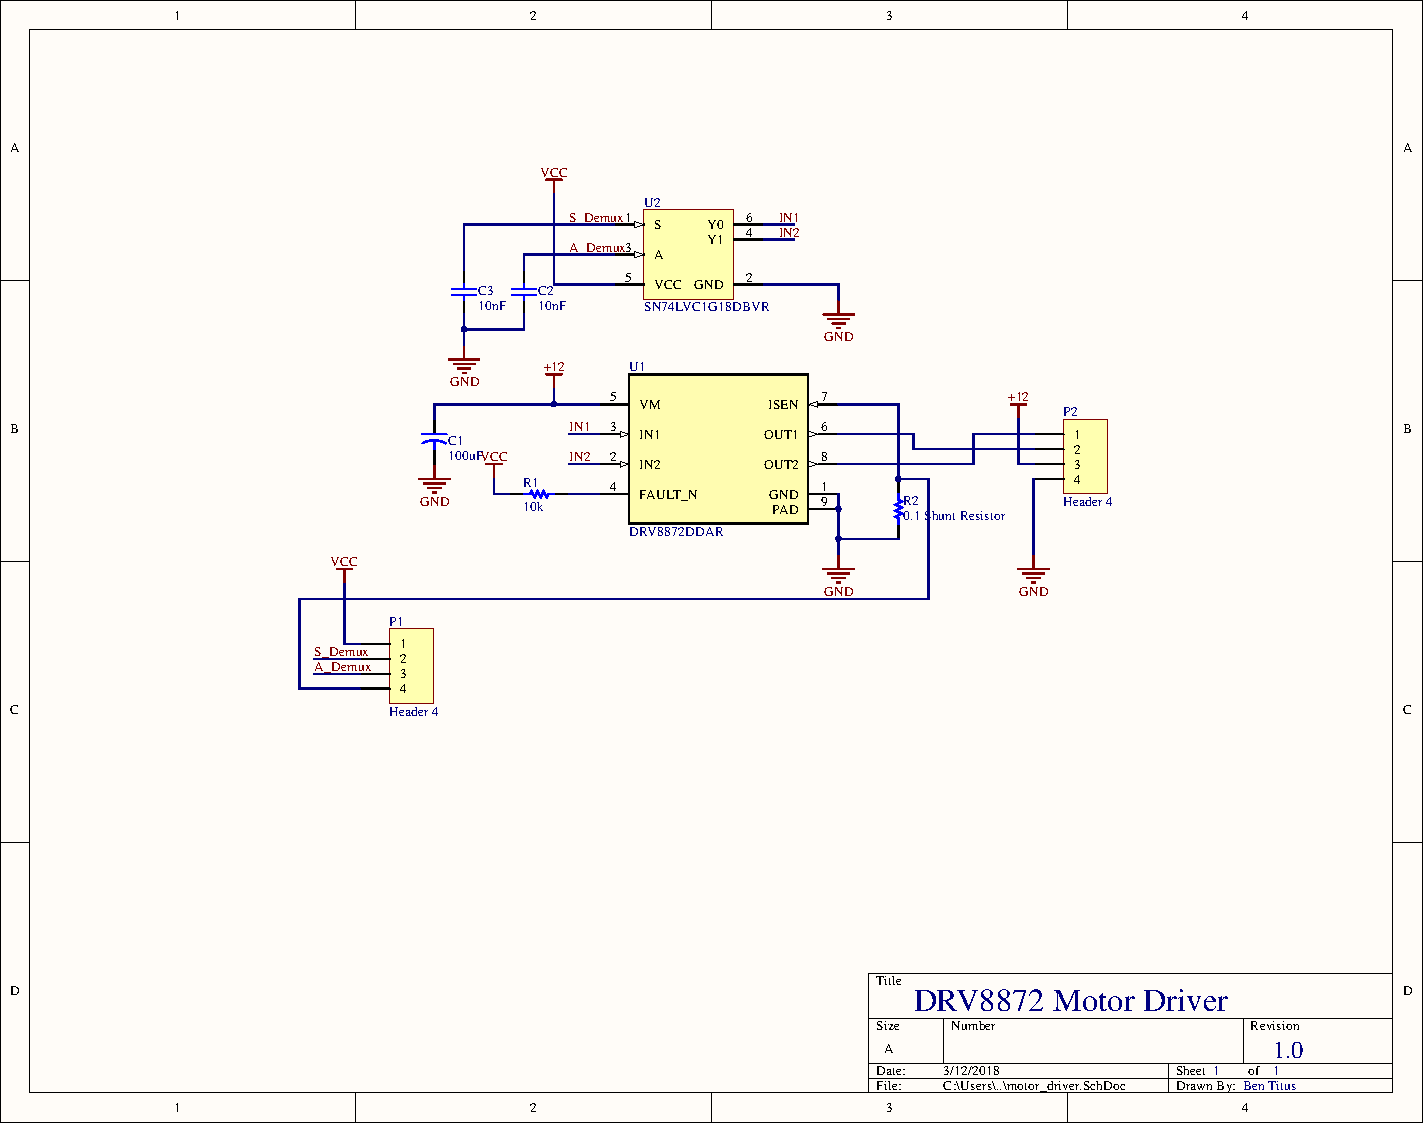
\includegraphics[page=1,width=\textwidth,angle=270]{PDFs/motor_driver.PDF} \newpage
\includegraphics[page=2,width=\textwidth,angle=270]{PDFs/motor_driver.PDF} \newpage 
\includegraphics[page=3,width=\textwidth,angle=270]{PDFs/motor_driver.PDF} \newpage
\pagenumbering{arabic}% resets `page` counter to 1
\renewcommand*{\thepage}{C\arabic{page}}
\begin{flushleft}
\section{Motor Driver with Current Sensor}
\end{flushleft}
\label{app:motor_driver_current}
\centering
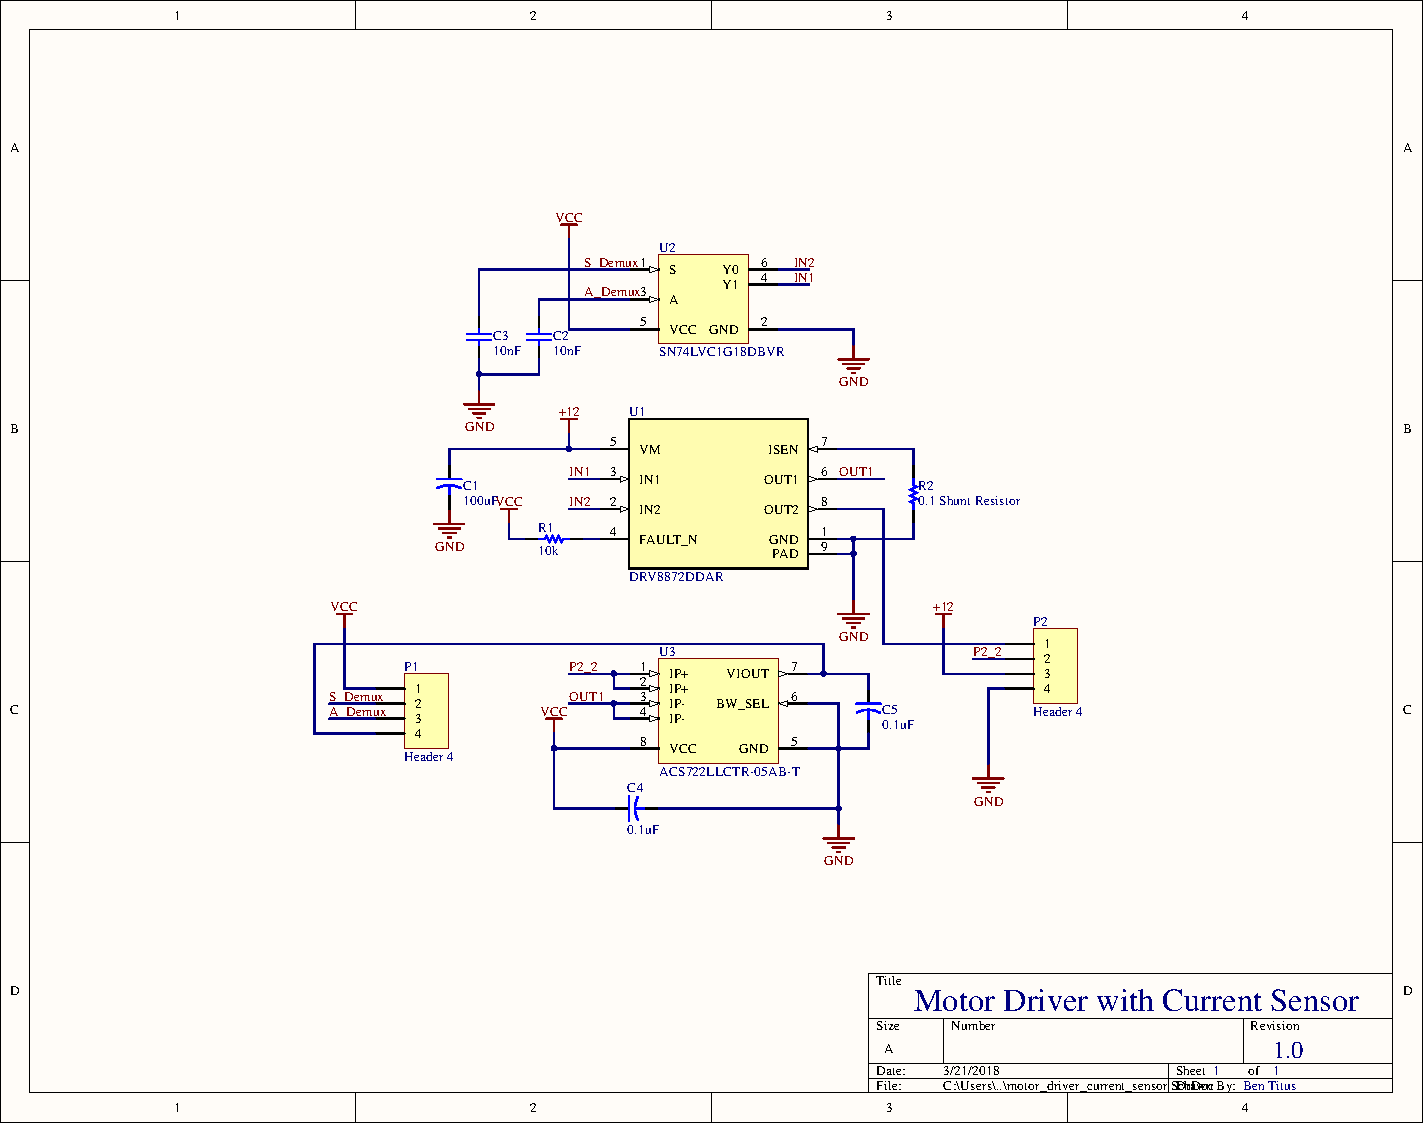
\includegraphics[page=1,width=\textwidth,angle=270]{PDFs/motor_driver_with_current_sensor.PDF} \newpage
\includegraphics[page=2,width=\textwidth,angle=270]{PDFs/motor_driver_with_current_sensor.PDF} \newpage
\includegraphics[page=3,width=\textwidth,angle=270]{PDFs/motor_driver_with_current_sensor.PDF} \newpage
\pagenumbering{arabic}% resets `page` counter to 1
\renewcommand*{\thepage}{D\arabic{page}}
\begin{flushleft}
\section{Load Cell Amplifier}
\end{flushleft}
\label{app:load_cell_amp}
\begin{figure}[H]
	\centering
	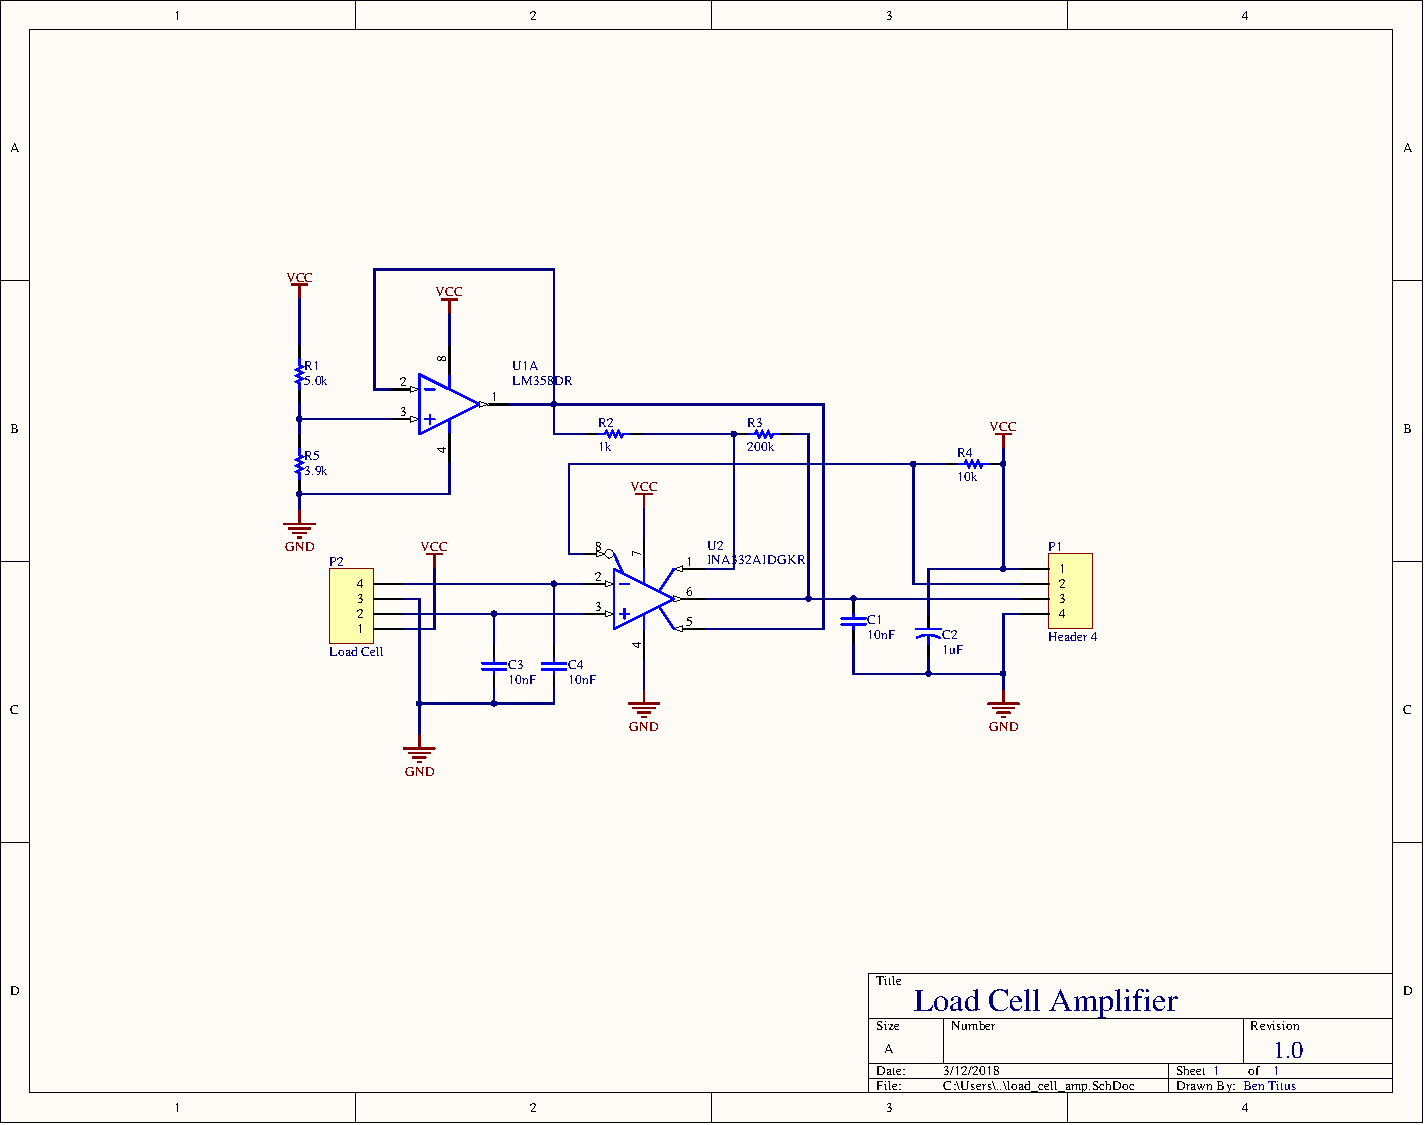
\includegraphics[page=1,scale=0.8,angle=270]{PDFs/load_cell_amp.PDF}
	\caption{Circuit diagram for load cell amplifier PCB}
	\label{fig:load_cell_amp_circuit}
\end{figure}
\begin{figure}[H]
	\centering
	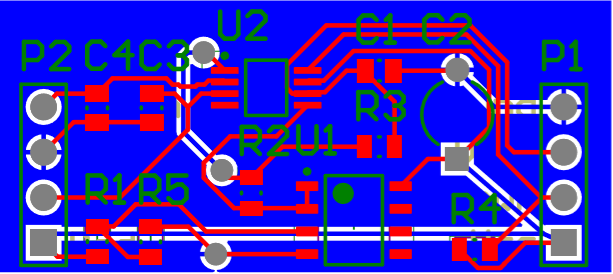
\includegraphics[scale=1]{load_cell_amp} 
	\caption{PCB composite for the load cell amplifier PCB}
	\label{fig:load_cell_amp_pcb}
\end{figure}
\begin{figure}[H]
	\centering
	\includegraphics[page=3,width=\textwidth]{PDFs/load_cell_amp.PDF} 
	\caption{Bill of materials for the load cell amplifier PCB}
	\label{fig:load_cell_amp_bom}
\end{figure}
\pagenumbering{arabic}% resets `page` counter to 1
\renewcommand*{\thepage}{E\arabic{page}}
\begin{flushleft}
\section{CAN Transceiver}
\end{flushleft}
\label{app:can_transceiver}
\centering
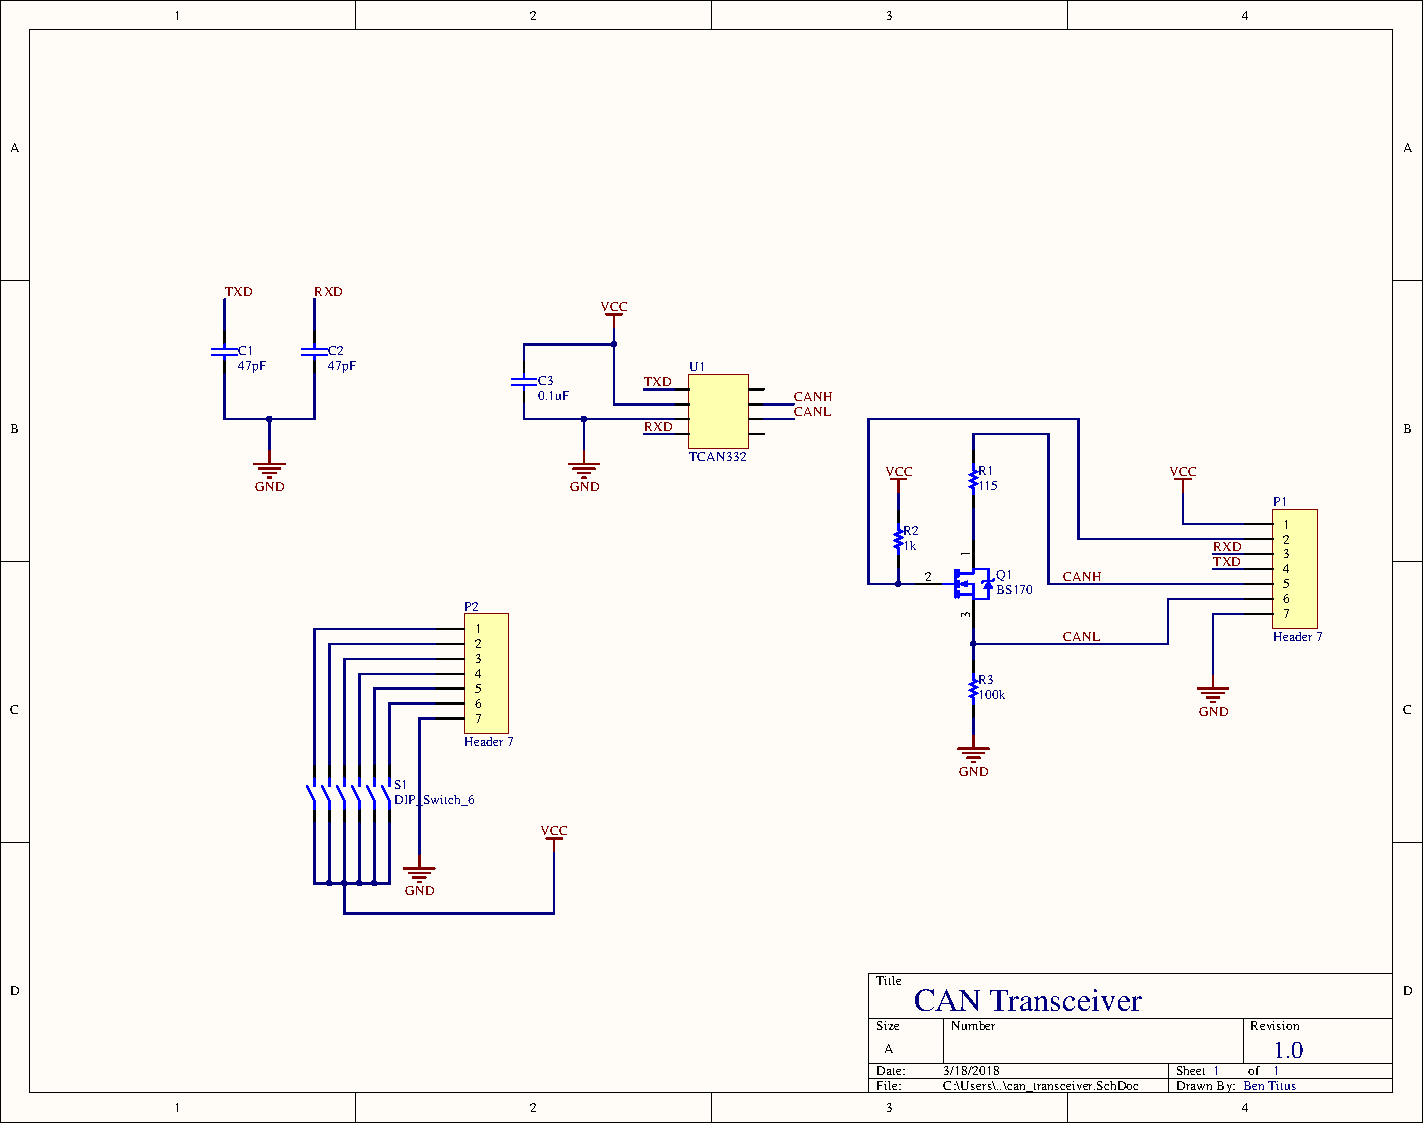
\includegraphics[page=1,width=\textwidth,angle=270]{PDFs/can_transceiver.PDF} \newpage
\includegraphics[page=2,width=\textwidth,angle=270]{PDFs/can_transceiver.PDF} \newpage
\includegraphics[page=3,width=\textwidth,angle=270]{PDFs/can_transceiver.PDF} \newpage
\pagenumbering{arabic}% resets `page` counter to 1
\renewcommand*{\thepage}{F\arabic{page}}
\section{Joint Board Boosterpack}
\label{app:joint_board_boosterpack}
\centering
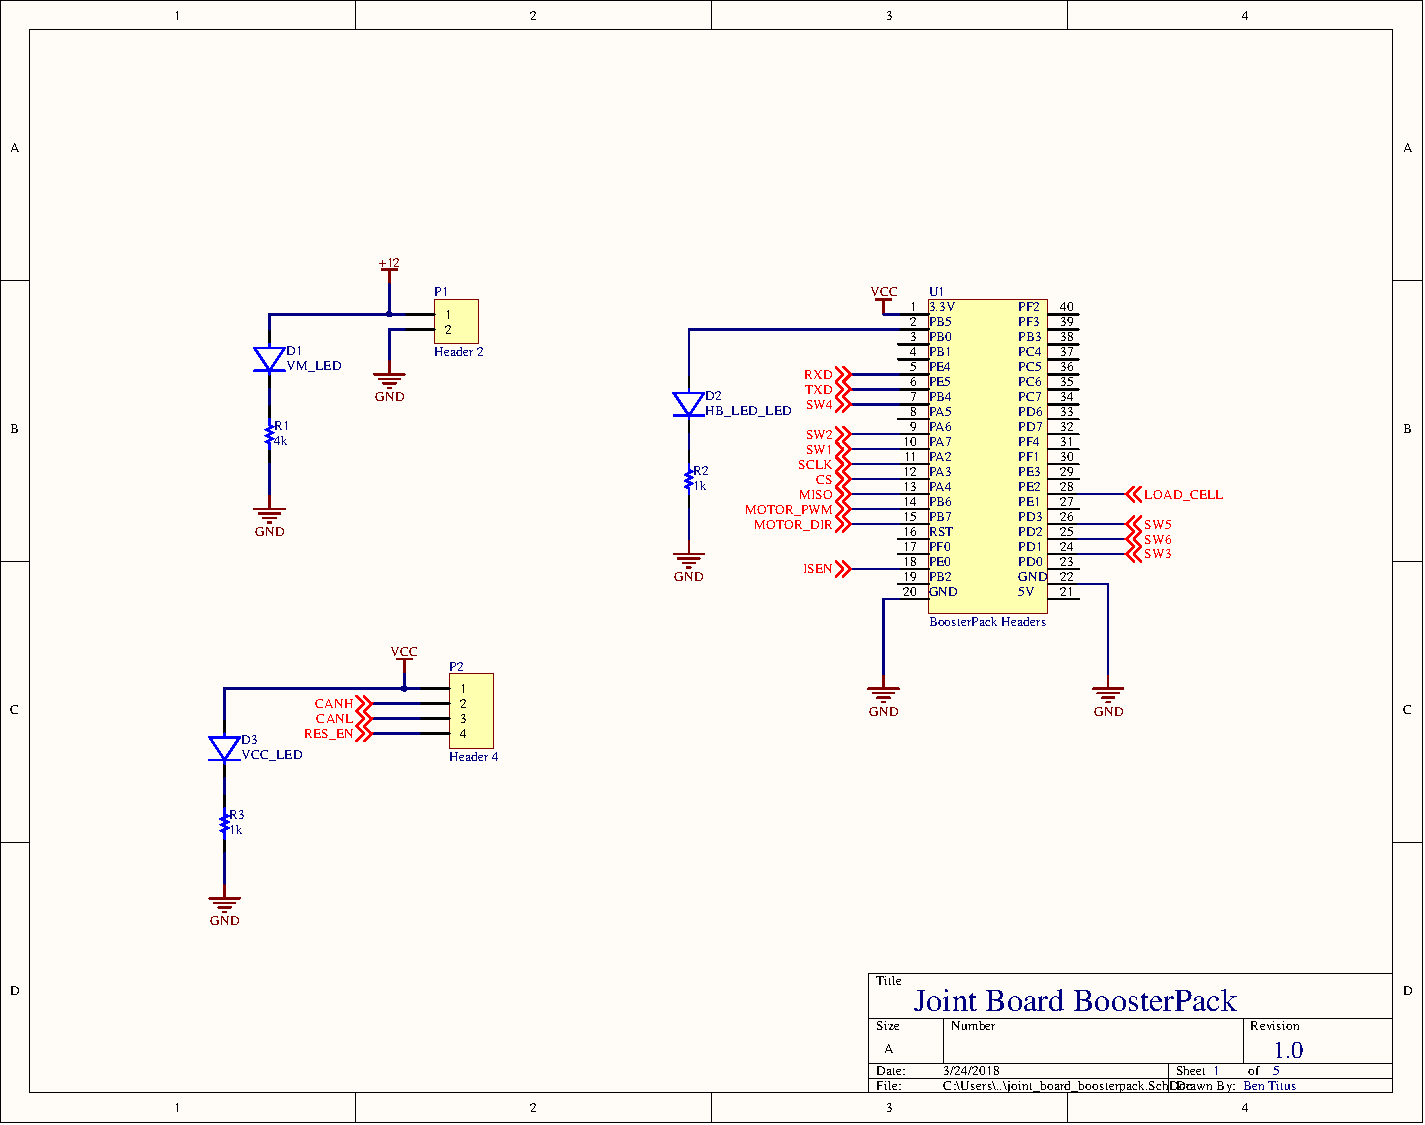
\includegraphics[page=1,width=\textwidth,angle=270]{PDFs/joint_board_boosterpack.PDF} \newpage
\includegraphics[page=2,width=\textwidth,angle=270]{PDFs/joint_board_boosterpack.PDF} \newpage
\includegraphics[page=3,width=\textwidth,angle=270]{PDFs/joint_board_boosterpack.PDF} \newpage
\includegraphics[page=4,width=\textwidth,angle=270]{PDFs/joint_board_boosterpack.PDF} \newpage
\includegraphics[page=5,width=\textwidth,angle=270]{PDFs/joint_board_boosterpack.PDF} \newpage
\includegraphics[page=6,width=\textwidth,angle=270]{PDFs/joint_board_boosterpack.PDF} \newpage
\includegraphics[page=7,width=\textwidth,angle=270]{PDFs/joint_board_boosterpack.PDF} \newpage
\pagenumbering{arabic}% resets `page` counter to 1
\renewcommand*{\thepage}{G\arabic{page}}
\begin{flushleft}
\section{TM4C123GH6PM Dev Board}
\end{flushleft}
\label{app:tm4c_dev_board}
\begin{center}
\includegraphics[page=1,width=\textwidth,angle=270]{PDFs/tm4c123_dev_board.PDF} \newpage
\includegraphics[page=2,width=\textwidth,angle=270]{PDFs/tm4c123_dev_board.PDF} \newpage
\includegraphics[page=3,width=\textwidth,angle=270]{PDFs/tm4c123_dev_board.PDF} \newpage
\end{center}
\pagenumbering{arabic}% resets `page` counter to 1
\renewcommand*{\thepage}{F\arabic{page}}
\begin{flushleft}
\section{Solidworks Drawings}
\end{flushleft}
\label{app:SolidworksDrawings}
<<<<<<< HEAD
\centering
\includegraphics[width=\textwidth,angle=270]{Solidworks/bottom_plate} \newpage
\includegraphics[width=\textwidth,angle=270]{Solidworks/bottom_plate_cradle} \newpage
\includegraphics[width=\textwidth,angle=270]{Solidworks/d_shaft_reciever} \newpage
\includegraphics[width=\textwidth,angle=270]{Solidworks/end_effector_mount} \newpage
\includegraphics[width=\textwidth,angle=270]{Solidworks/end_of_arm} \newpage
\includegraphics[width=\textwidth,angle=270]{Solidworks/idler_shaft} \newpage
\includegraphics[width=\textwidth,angle=270]{Solidworks/main_shaft} \newpage
\includegraphics[width=\textwidth,angle=270]{Solidworks/servo_horn_connector} \newpage
\includegraphics[width=\textwidth,angle=270]{Solidworks/sidewall} \newpage
\includegraphics[width=\textwidth,angle=270]{Solidworks/top_plate} \newpage
=======
\begin{center}
\includegraphics[page=1,width=\textwidth,angle=270]{Solidworks/bottom_plate} \newpage
\end{center}
>>>>>>> 0963b70607e29d33a0c5eb4ec05c9defafe603a1



\end{appendices}

\end{document}